%! TEX root = main.tex
\section{Evoluzione stellare}\linkdest{stellarevolution}

\subsection{Pre-MS}

\begin{wordonframe}{da fare: kippenhahn wiegert}
	\begin{itemize}
		\item Hayashi line 224'-232' (119-123)
		\item pre-main sequence contraction 266'-270' (140-142)
	\end{itemize}
\end{wordonframe}

\begin{frame}{Traccia d'Hayashi: protostar can be described by SSE}
	\begin{columns}[T]
		\begin{column}{0.50\textwidth}
            \begin{figure}[!ht]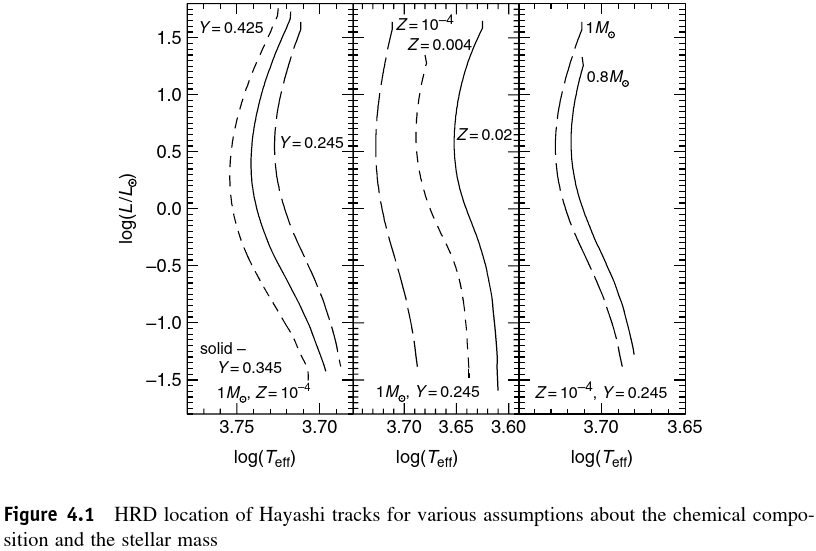
\includegraphics[trim={0.6cm 0cm 1.1cm 0},clip, keepaspectratio,width=0.95\textwidth]{hayatrack}
			\end{figure}
		\end{column}
		\begin{column}{0.50\textwidth}
            \begin{itemize}
                    \item $\log{T_e}=A\log{L}+B\log{M}+\const{}$: $\TDly{T_e}{L}=\frac{1}{A}\gg1$ HL almost vertical, HL shift to left as \xaumenta{M}.
                    \item Extension of superadiabatic layer and ionization zones varies with $L$: $A>0$ for low L and changes sign at $L\approx\lsun$: see effects of superadiabatic convection and depression of $\nabla_{Ad}$ in next.
                    \item Fully convective star model as contracting polytrope with no nuclear source, $n=\frac{1}{\nabla_{Ad}}-1=\frac{3}{2}$, $P=CT^{n+1}$: on HL $\exv{\nabla}=\nabla_{Ad}$, close to HL $\exv{\nabla}=\invers{(1+n)}$, $\PDy{n}{\log{T_e}}>0$ star move to right as $n$ decreases ($\exv{\nabla}$ increases, in a model to the left of HL the radiative part decreases average value $\exv{\nabla}<\nabla_{Ad}$).
                \end{itemize}
		\end{column}
	\end{columns}
    Considering contracting polytrope, energy generation rate prop. to $T$, for ideal monoatomic gas in homologous contraction $\epsilon_g=-\frac{3}{5}c_PT \frac{\dot{R}}{R}$; assuming $\frac{l}{m}=\frac{L}{M}=\const{}$, $n=1.5$ ($\nabla=\nabla_{Ad}=0.4$), opacity law $\kappa=\kappa_0P^aT^b$ for Kramer's opacity $a=1$, $b=-4.5$: $\nrad\propto\frac{\kappa l P}{T^4m}\propto\frac{L}{M}C^{1+a}T^{b-4+2.5(1+a)}$ so $\nrad{}\propto T^{-3.5}$. For reas.op. $\nrad{}$ has minimum at center and increases outward: is first point where $\nrad{<\nad{}}$ if L decreases below a $L_{min}$; as $C=C'R^{-\frac{3}{2}}M^{-\frac{1}{2}}$ and $T\propto T_c\propto \frac{M}{R}$: $\nrad{}\propto LM^{b-5+2(1+a)}R^{-b+4-4(1+a)}\to LM^{-5.5}R^{0.5}$. For model on HL $T_e\approx\const{}$ so $R\propto L^{\frac{1}{2}}$: $\nrad{}\propto L^{1.25}M^{-5.5}$, for any given M $L=L_{min}$ when $\nad{}=0.4$ at center and $L_{min}\propto M^{4.4}$: this minimum luminosity down to which fully convective and very small mass star can cross main sequence without reaching $L_{min}$
\end{frame}

\begin{frame}[fragile]{HL: stelle completamente convettive. Fitting interior to photosphere conditions}
	\begin{columns}[T]
		\begin{column}{0.5\textwidth}
			Fully convective interior: $\nabla=\nad$, polytrope $P=CT^{n+1}$, ($n=\frac{1}{\nad}-1=\frac{3}{2}$), $P=\frac{R\rho T}{\mu}$, photosphere at $\tau=\frac{2}{3}$, $P_0$, $T_e$, $R$, $M$
			\[\log{T}=0.4\log{P}+0.4(\frac{3}{2}\log{R}+\frac{1}{2}\log{M}-\log{C'})\]
			Atmosphere (Radiative): $\exv{\kappa}\propto\kappa_0T^bP^a$, $\tau=\int_R^{\infty}$, HE: $P(r=R)=\int_R^{\infty}g\rho\,dr=g_0\int_R^{\infty}\rho\,dr=\frac{GM}{R^2}\frac{2}{3\exv{\kappa}}$:
			\[(a+1)\log{P_0}=\log{M}-2\log{R}-b\log{T_e}+\const{}\]
			%$P_0\propto(\frac{M}{R^2}T_e^{-b})^{\frac{1}{1+a}}$
			Low $T_e$: atmospheric opacity from $H^-$: $A\approx0.05$, $B\approx0.2$
			HL neighborhood: the larger $T_e$ the earlier radiative region before the center ($\exv{\nabla}<\nad$), on the right of HL $\exv{\nabla}>\nad$ (super-adiabatic convection in interior: star goes to the left with convective/dynamical timescale).	
		\end{column}
		\begin{column}{0.45\textwidth}
			\begin{figure}[!ht]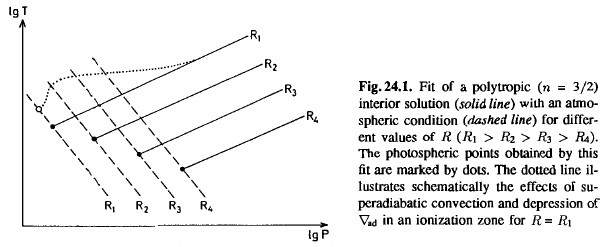
\includegraphics[trim={0cm 0cm 0 0},clip, keepaspectratio,width=0.90\textwidth]{HL-intatm}\label{fig:HL-intatm}
			\end{figure}
			\begin{figure}[!ht]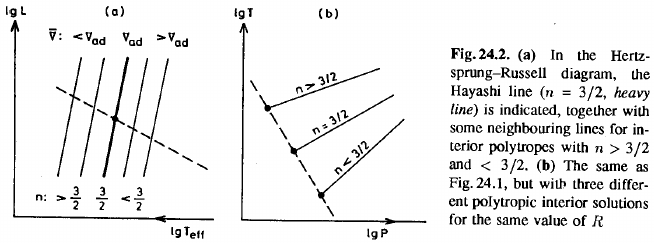
\includegraphics[trim={0cm 0cm 0 0},clip, keepaspectratio,width=0.90\textwidth]{HL-fulladiabatneigh}\label{fig:HL-fulladiabatneigh}
		\end{figure}
		\end{column}
	\end{columns}
\end{frame}

\begin{frame}{Burning of light elements in pre-MS (Hartmann97, Tognelli 2017)}
    \begin{columns}[T]
        \begin{column}{0.5\textwidth}
    Contrazione su $\tau\approx\tkh{}$ fino a innesco reazioni nucleari, in cui $L\propto t^{-\frac{2}{3}}$; nel caso si raggiungano le temperature di soglia per elementi leggeri si arresta contrazione ($\tau\approx\tau_n$).
            \begin{align*}
                &p(^2H,\APelectron\nu)^3He\tag{$T\approx\SI{e6}{\kelvin}$}\\
                &p(^6Li,^3He)^4He\tag{$T\approx\SI{2e6}{\kelvin}$}\\
                &p(^7Li,^4He)^4He\tag{$T\approx\SI{2.5e6}{\kelvin}$}\\
                &p(^9Be,^4He)^6Li\tag{$T\approx\SI{3.5e6}{\kelvin}$}\\
                &p(^{10}B,^4He)^7Be\tag{$T\approx\SI{4.5e6}{\kelvin}$}\\
                &p(^{11}B,2 ^4He)^4He\tag{$T\approx\SI{5e6}{\kelvin}$}
            \end{align*}
            $T_{Th}(X_i)>T_{bcz}$: Elemento $X_i$ non viene bruciato.
        \end{column}
        \begin{column}{0.5\textwidth}
			\begin{figure}[!ht]
                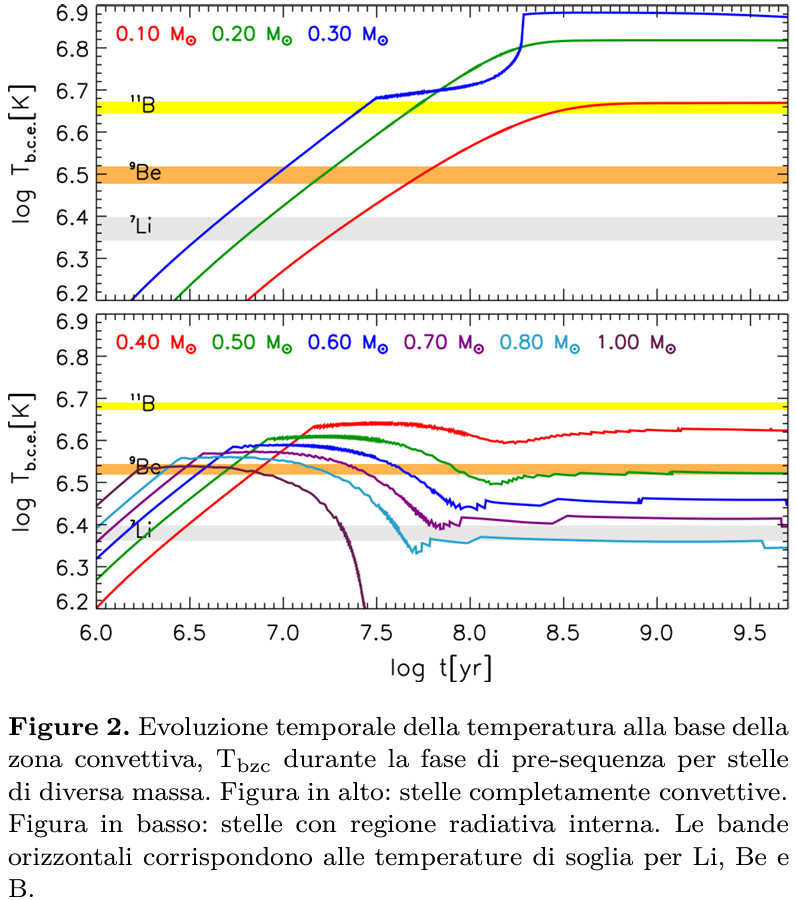
\includegraphics[trim={0cm 0cm 0 0},clip, keepaspectratio,height=0.45\textheight]{preMS-Tbcz}\label{fig:preMS-Tbcz}
			\end{figure}
        \end{column}
    \end{columns}
    
			\begin{figure}[!ht]
                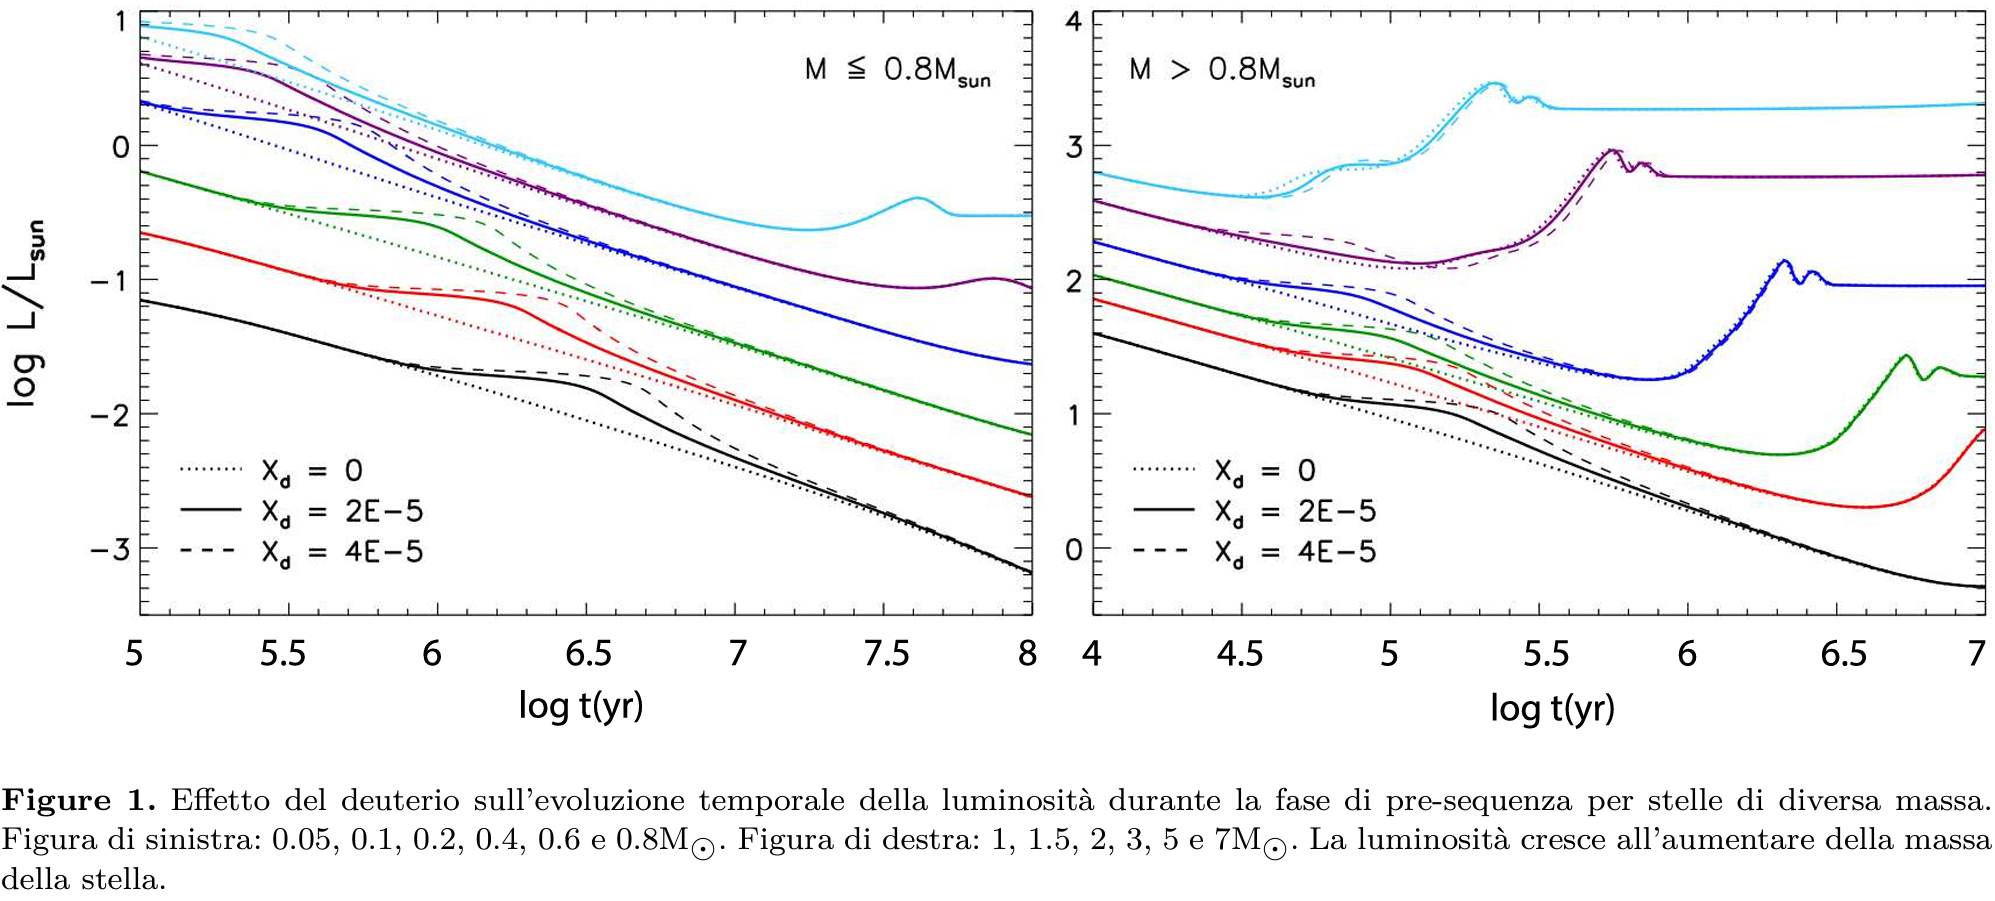
\includegraphics[trim={0cm 0cm 0 0},clip, keepaspectratio,height=0.45\textheight]{preMS-L}\label{fig:preMS-L}
			\end{figure}
\end{frame}

\subsection{Evoluzione di sequenza principale}\linkdest{MS}

\begin{frame}{Approccio alla ZAMS per stelle di sequenza superiori/inferiori}
dipendenza della ZAMS dall'abbondanza originale di He e metalli; metodo determinazione $DY/DZ$ dal confronto teoria-osservazione per stelle di disco locale parallassate; dipendenza massa minima di transizione dall'abbondanza di He e metalli; influenza sulla ZAMS dell'incertezza degli input fisici e dell'efficienza della convezione
\end{frame}

\begin{frame}{Yield of H-burning star analysis}
    \begin{columns}[T]
        \begin{column}{0.5\textwidth}
    \begin{itemize}
\item Longest evolutionary phase: larger number of observed stars
\item central/shell-H-burning determine successive phases
\item most important clock is central H-burning termination
\item Final shell H-burning phase in low mass, low-Z star provide distance indicator for old stellar pop
\item count of stars evolving through central H-burning give insight on IMF
\end{itemize}
        \end{column}
        \begin{column}{0.5\textwidth}
            \begin{figure}[!ht]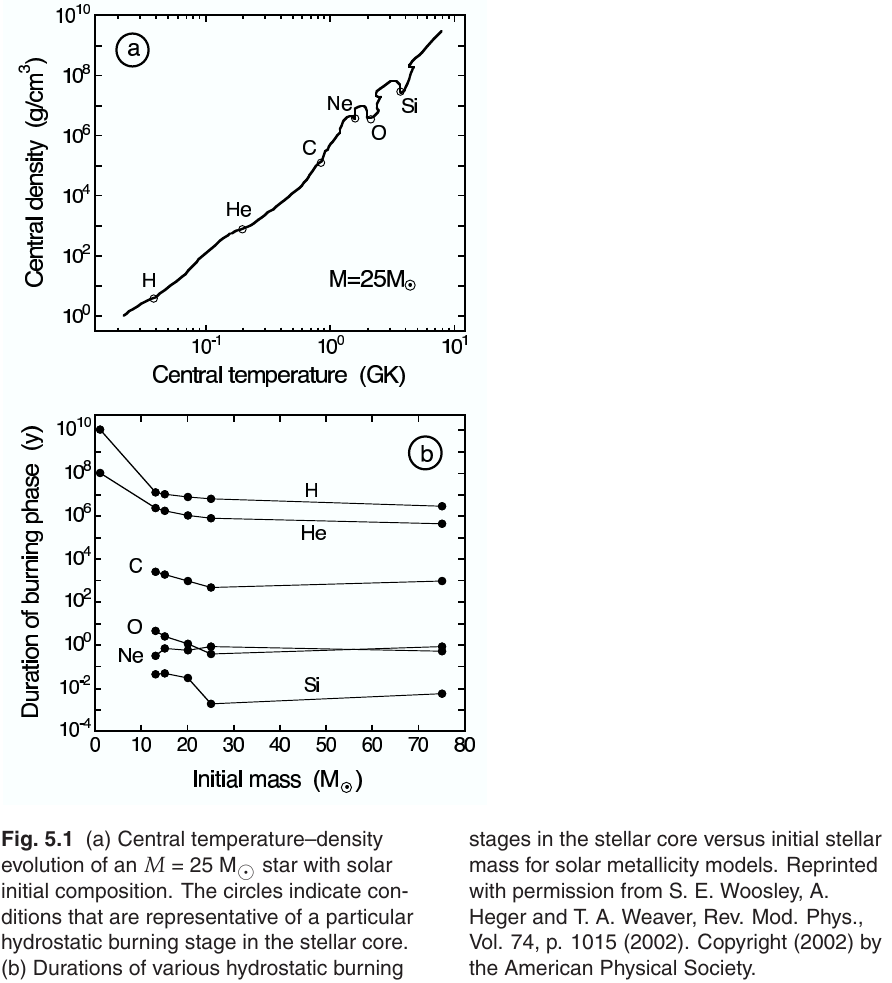
\includegraphics[trim={0.0cm 0cm 0.0cm 0},clip, keepaspectratio,width=0.95\textwidth]{burninglifetime}
			\end{figure}
        \end{column}
    \end{columns}
    
\end{frame}

\begin{frame}[fragile]{Major H burning reaction: PP chains}
\begin{columns}[T]\begin{column}{0.35\textwidth}
\begin{align*} 
&T\geq\SI{5e6}{\kelvin}\\
&^1H+^1H\to^2D+\APelectron+\Pnue\\
&^2D+^1H\to^3He+\gamma\\
&T\geq\SI{8e6}{\kelvin}:\\
&^3He+^3He\to^4He+2^1H\tag*{PPI}\\
&T\geq\SI{15e6}{\kelvin}:\\
&^3He+^4He\to^7Be+\gamma\\
&^7Be+\Pelectron\to^7Li+\Pnue\\
&^7Li+^1H\to^4He+^4He\tag*{PPII}\\
&^7Be+^1H\to^8B+\gamma\\
&^8B\to^8Be+\APelectron+\Pnue\\
&^8Be\to2^4He\tag*{PPIII}
\end{align*}
\end{column}\begin{column}{0.65\textwidth}
\begin{comment} 
\begin{align*}
&r_{pp}=\num{11.5e10}\rho^2X_H^2T_6\expy{-2/3}\\
&\exp{-33.81T_6\expy{-1/3}}(1+\num{0.0123}T_6\expy{1/3}+\num{0.0109}T_6\expy{2/3}\\
&+\num{0.00095}T_6)\\
&\rho\epsilon(3H\to^3He)=\\
&(\SI{6.936}{\mega\ev}-\SI{0.263}{\mega\ev})*\SI{1.602e-6}{\erg}*r_{pp}\\
&\rho\epsilon(^3He(^3He,2p)^4He)=\\
&(\SI{6.936}{\mega\ev}-\SI{0.263}{\mega\ev})*\SI{1.602e-6}{\erg}*r_{pp}\\
&\frac{PPI}{PPII+PPIII}=\frac{r_{33}}{r_{34}}=\frac{\lambda_{33}(^3He)^2/2}{\lambda_{34}^3He^4He}
\end{align*} 
\end{comment}
\begin{itemize}
    \item $Q=4*\massexcess{H}-\massexcess{^4He}=4*\SI{7288.97}{\kilo\ev}-\SI{2424.92}{\kilo\ev}=\SI{26.731}{\mega\ev}$ - energy release per gram $Q/m(^4He)=\SI{6.4e18}{\erg\per\gram}$ (Mass-excess: $\Delta m(A,Z)=M(A,Z)-A*u$)
    \item Energia nucleare: $n_p\approx \frac{\msun{}X}{m_p}\approx \frac{\num{2e33}*0.7}{\num{1.67e-24}}\approx\num{e57}$ protons, $E_{nucl}\approx \frac{\num{e57}\SI{26.1}{\mega\ev}}{4}\approx\SI{6e57}{\mega\ev}$
    \item Neutrino's Flux: $\Phi_{\nu}=\frac{n_{\nu}}{4\pi D^2}=\frac{2 \frac{\lsun{}}{\SI{26.1}{\mega\ev}}}{4\pi D^2}=\frac{\num{1.9e38}\nu/s}{\num{2.82e27}}\approx \frac{\num{6.7e10}\nu}{\si{\square\cm\second}}$, $\lsun{}\approx\SI{2.5e39}{\mega\ev\per\second}$
\item Neutrino releases: PPI - \SI{0.5}{\mega\ev} per He
\item Neutrino releases: PPII - \SI{0.81}{\mega\ev} per He
\item Neutrino releases: PPI - \SI{6.71}{\mega\ev} per He
\item $\epsilon_{PP}\propto X^2\rho T^4$
\end{itemize}
\end{column}\end{columns}
\end{frame}

\begin{frame}{H burning: CN-NO cycle}
\begin{columns}[T]\begin{column}{0.4\textwidth}
        Ciclo CN-NO: $T\geq\SI{1.5e7}{\kelvin}$
\begin{align*}
&^{12}C+^1H\to^{13}N+\gamma\\
&^{13}N\to^{13}C\APelectron+\Pnue\\
&^{13}C+^1H\to^{14}N+\gamma\\
&^{14}N+^1H\to^{15}O+\gamma\\
&^{15}O\to^{15}N+\APelectron+\Pnue\\
&^{15}N+^1H\to^{12}C+^4He\tag*{CN}\\
&T\geq\SI{20e6}{\kelvin}\tag*{Branching Ratio: \num{e-4}}\\
&^{15}N+^1H\to^{16}O+\gamma\\
&^{16}O+^1H\to^{17}F+\gamma\\
&^{17}F\to^{17}O+\APelectron+\Pnue\\
&^{17}O+^1H\to^{14}N+^4He\\
&^{17}O(p,\gamma)^{18}F\tag{$1\%$}\\
&^{18}F\to^{18}O\APelectron\Pnue\\
&^{18}O(p,\alpha)^{15}N\\
&^{18}O(p,\gamma)^{19}F\\
&^{19}F(p,\alpha)^{16}O\\
&^{19}F(p,\gamma)^{20}Ne
\end{align*} 
\end{column}\begin{column}{0.6\textwidth}
    Chemical changes: (CN) \xdiminuisce{C},\xaumenta{N}; (CNO) \xdiminuisce{C}, \xaumenta{N}, \xdiminuisce{O}.
    \begin{align*}
&\epsilon_{CN}(T_6)=\epsilon_{CN}(25)(\frac{T_6}{25})^{16.7}\\
&\epsilon_{CNO}\propto XX_{14}\rho T^{18}\\
&
\end{align*}
Matter processed by CN: \xdiminuisce{C}, \xaumenta{N}; by CNO: \xdiminuisce{C}, \xaumenta{N}, \xdiminuisce{O}.
\end{column}\end{columns}
\end{frame} 

\subsection{Lower main sequence ($M^*\leq1.3\msun{}$)}\linkdest{LMS}

\begin{frame}{Da ZAMS a TO for $M^*\leq1.3\msun{}$}
ZAMS: first MS model fully supported by H-burning in which secondary elements are in equilibrium:
\begin{itemize}
\item $^3He$ production in central zones: si forma piccolo core convettivo
    \[\TDy{t}{N_{^3He}}=N_{^1H}N_D\exv{\sigma v}_{^1HD}-2\frac{(N_{^3He})^2}{2}\exv{\sigma v}_{^3He^3He}-N_{^3He}N_{^4He}\exv{\sigma v}_{^3He^4He}\]
    Assuming $N_{^3He}\gg N_{^3He}^{eq}$ we can estimate time scale for $^3He$ equilibrium.
\end{itemize}
\begin{columns}[T]\begin{column}{0.5\textwidth}
\begin{figure}[!ht]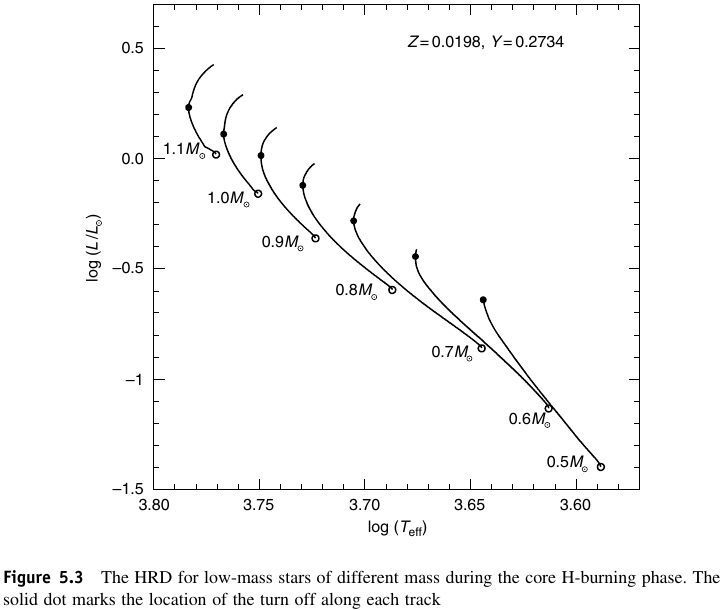
\includegraphics[trim={0cm 0cm 0 0},clip, keepaspectratio,width=0.99\textwidth]{HRD-LMS}\label{fig:HRD-LMS}
\end{figure}
\end{column}\begin{column}{0.50\textwidth}
    \begin{itemize}
        \item La stella continua a contrarsi fino alla partenza della reazione $^3He(^3He,2^1H)^4He$ e il core convettivo svanisce con l'espandersi della regione in cui \'e prodotto $^3He$
        \item Struttura: H-burn in central radiative core (Small T-dep of $\epsilon_{PP}$), convective envelope (large opacity associated to partial ionized H, He)
        \item Evoluzione: $\#$ free particles $\downarrow$, \xaumenta{\mu} per HE \xaumenta{T}, \xdiminuisce{R} quindi $L^*$ aumenta lentamente.
        \item TO is hottest point in evolutionary track: H exhausted 
\end{itemize}
\end{column}\end{columns}
\end{frame}


\subsection{Upper main sequence ($M^*\geq1.2-1.3\msun{}$)}\linkdest{UMS}

\begin{frame}{Da ZAMS a Overall contraction}
\begin{columns}[T]\begin{column}{0.5\textwidth}
\begin{figure}[!ht]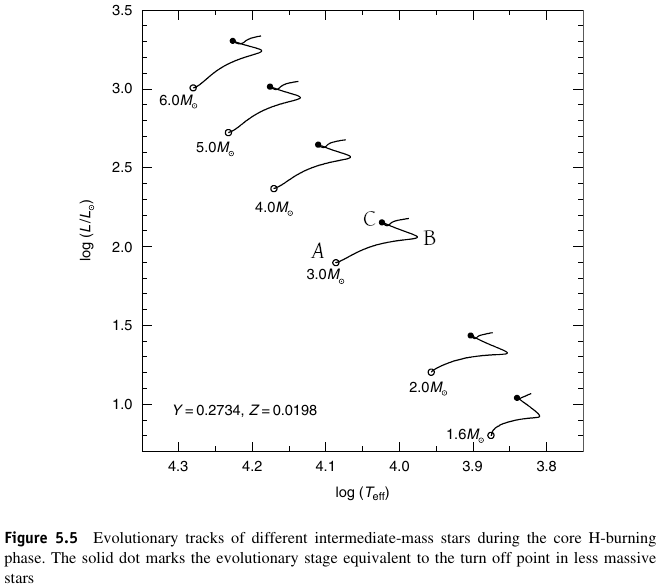
\includegraphics[trim={0cm 0cm 0 0},clip, keepaspectratio,width=0.7\textwidth]{HRD-UMS}\label{fig:HRD-UMS}
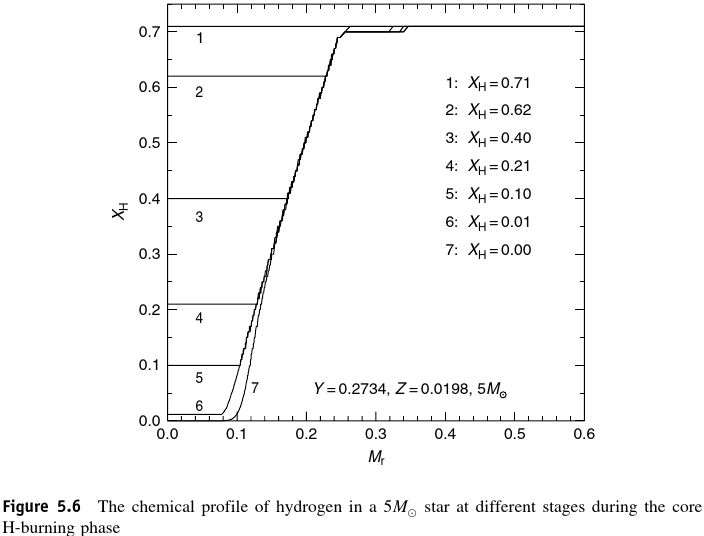
\includegraphics[trim={0cm 0cm 0 0},clip, keepaspectratio,height=0.40\textheight]{UMS-Hprofile}\label{fig:UMS-Hprofile}\end{figure}
\end{column}\begin{column}{0.5\textwidth}
\begin{block}{CNO H-Burning: convective core}
Higher T: CNO dominant: $\epsilon_{CNO}$ steeper:convective core: \xaumenta{M^*}, \xaumenta{M_{con}}, \xaumenta{P_{rad}}, \xdiminuisce{\nad{}}.
\end{block}
\begin{block}{As UMS burn H}
\begin{itemize}
    \item convective core shrink: ?\xaumenta{\mu}, \xaumenta{P_c}?
    \item radius expands: after H exhaustion
    \item core gravitationally contract
    \item $L$ increases such that $T_e$ has little drop
\end{itemize}
\end{block}
\begin{block}{Overall contraction}
    When $X<0.05$ at B start gravitational contraction of core until C; after C inner regions contract outer expand; C mark ends of central H-burning phase: after C core contracts and outer envelope expands and thus radius increases and outer opacity increases while T outer layers decreases.
\end{block}
\begin{block}{Core retraction leaves He gradient}
    Convective core retracts as X is strongly decreased leaving He gradient decreasing moving outwards.
\end{block}
\end{column}\end{columns}
\end{frame}

\begin{frame}{Details of $5\msun{}$}
    \begin{columns}[T]
        \begin{column}{0.6\textwidth}
\begin{figure}[!ht]
    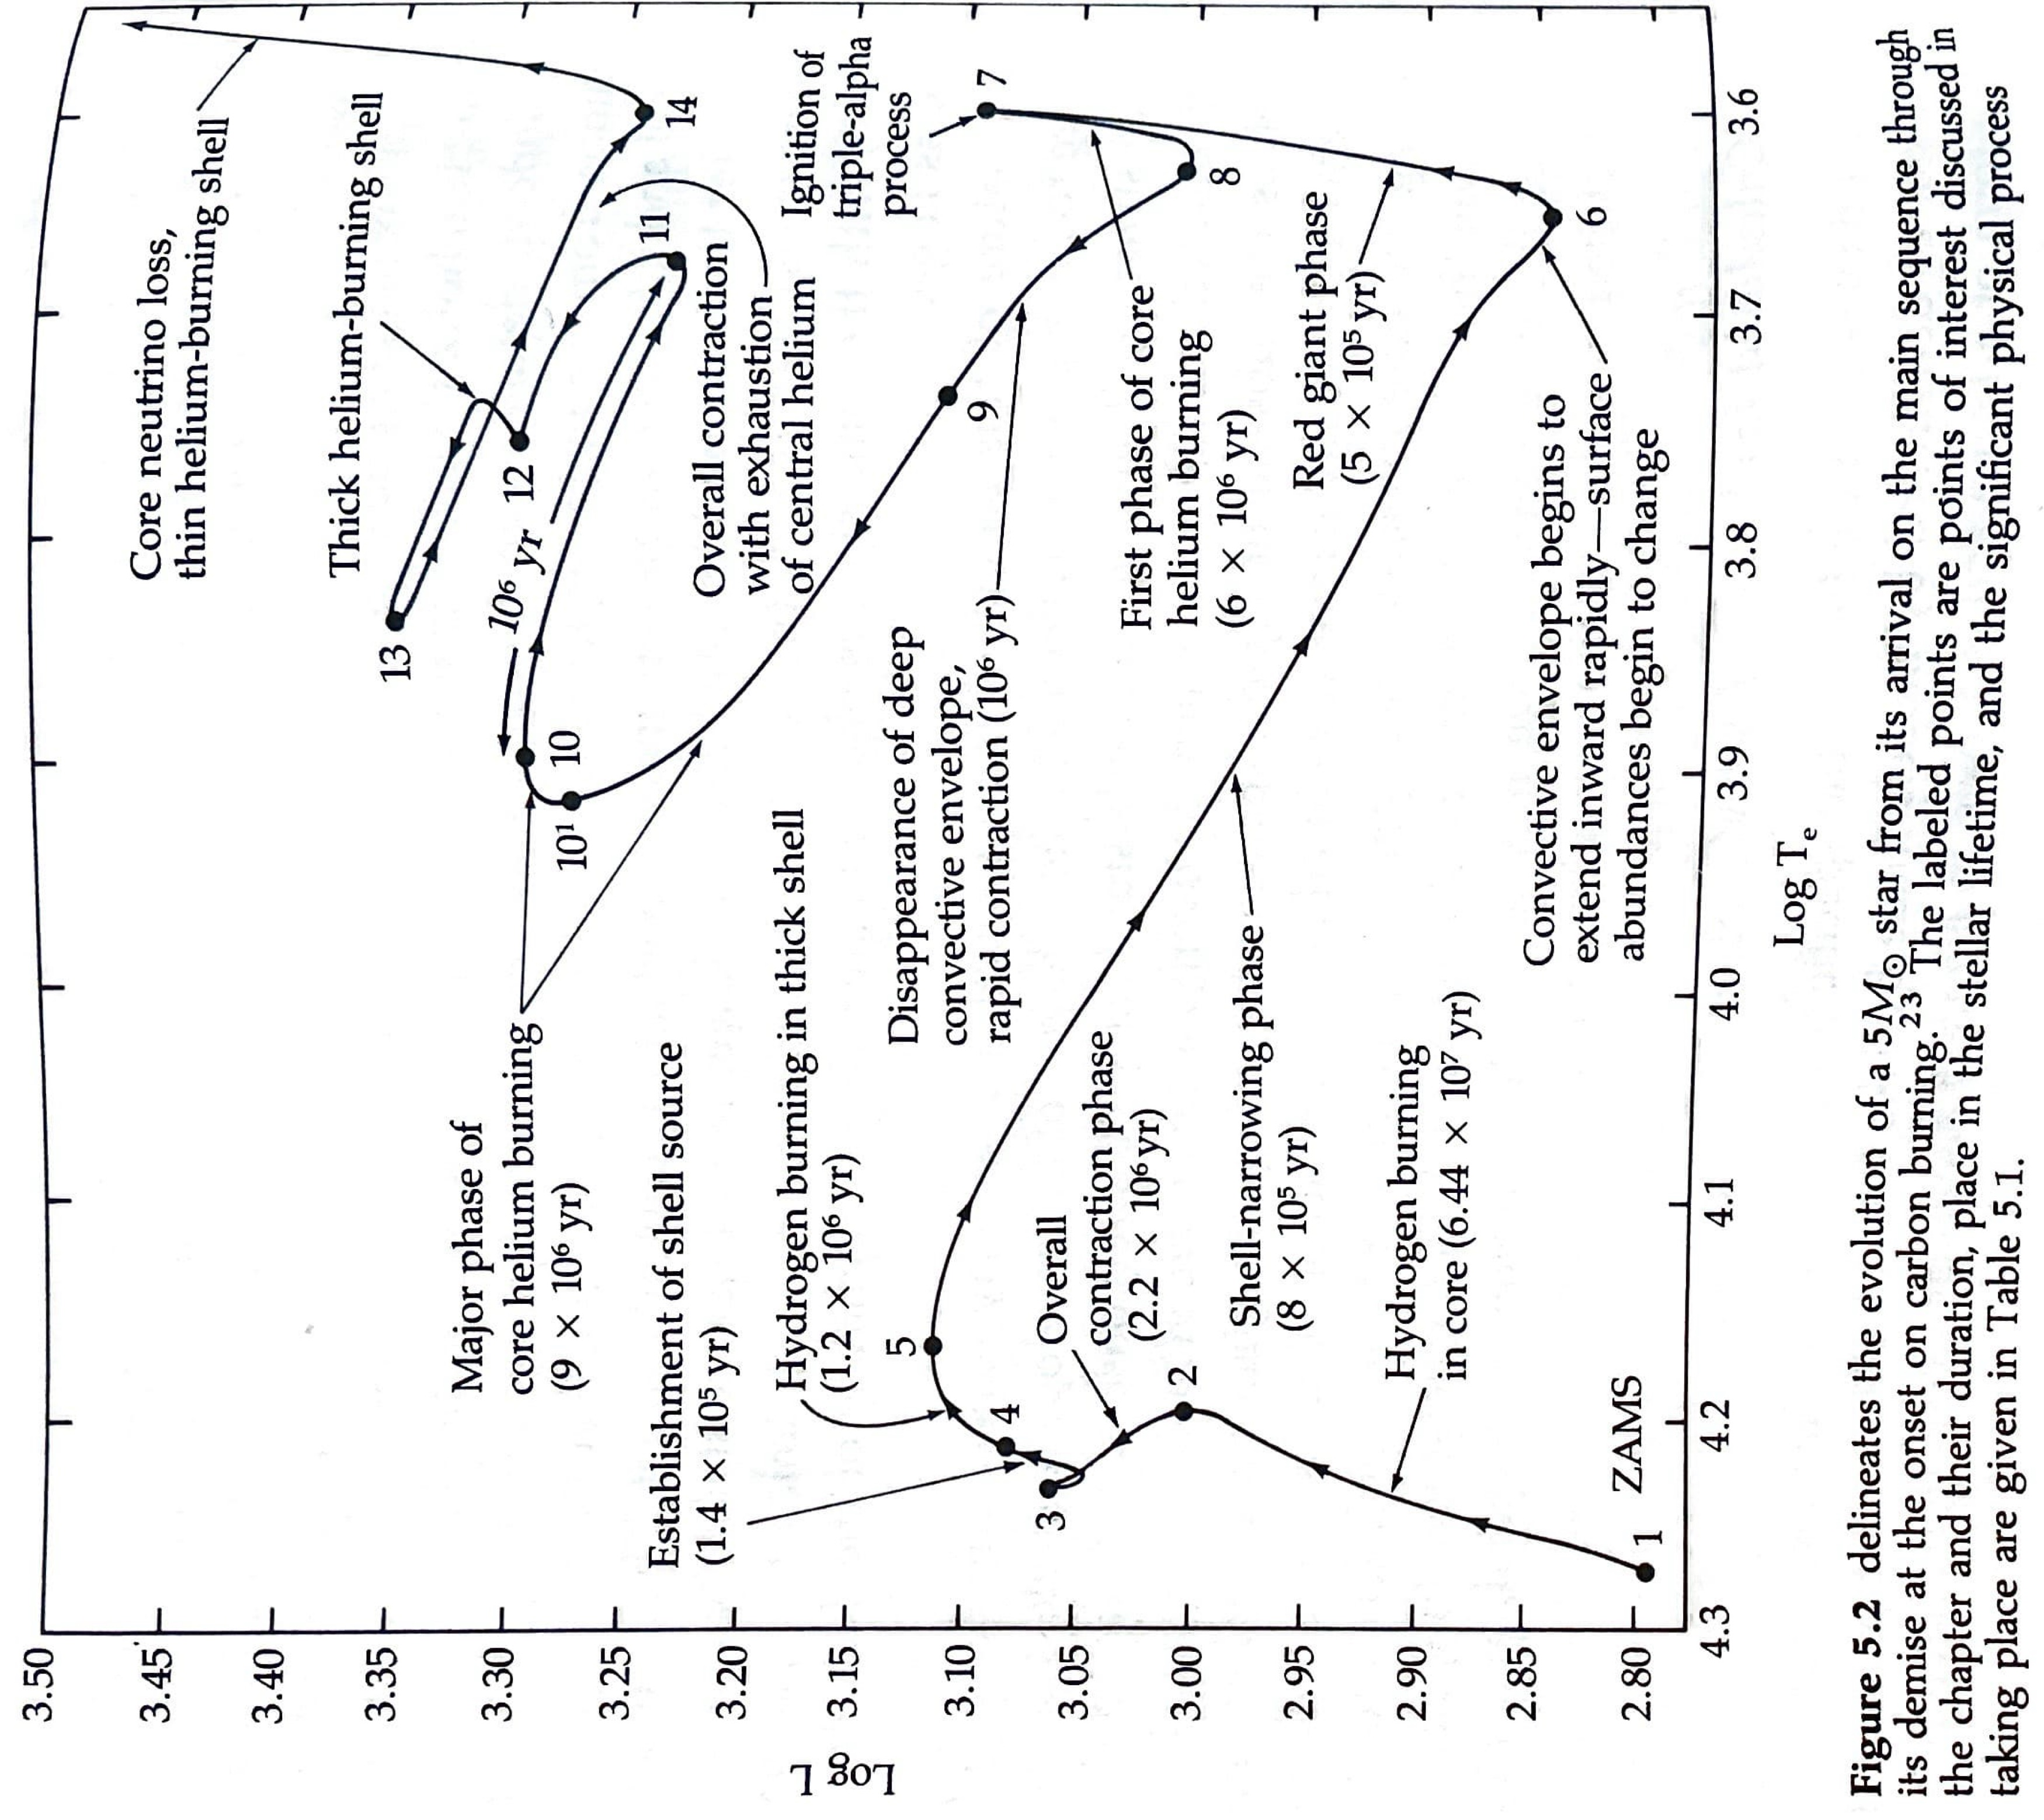
\includegraphics[trim={0cm 0cm 0 0},clip, keepaspectratio,height=0.8\textheight,origin=c,angle=-90]{5msun_detail}\label{fig:5msun_detail}
\end{figure}
        \end{column}
        \begin{column}{0.4\textwidth}
\begin{figure}[!ht]
    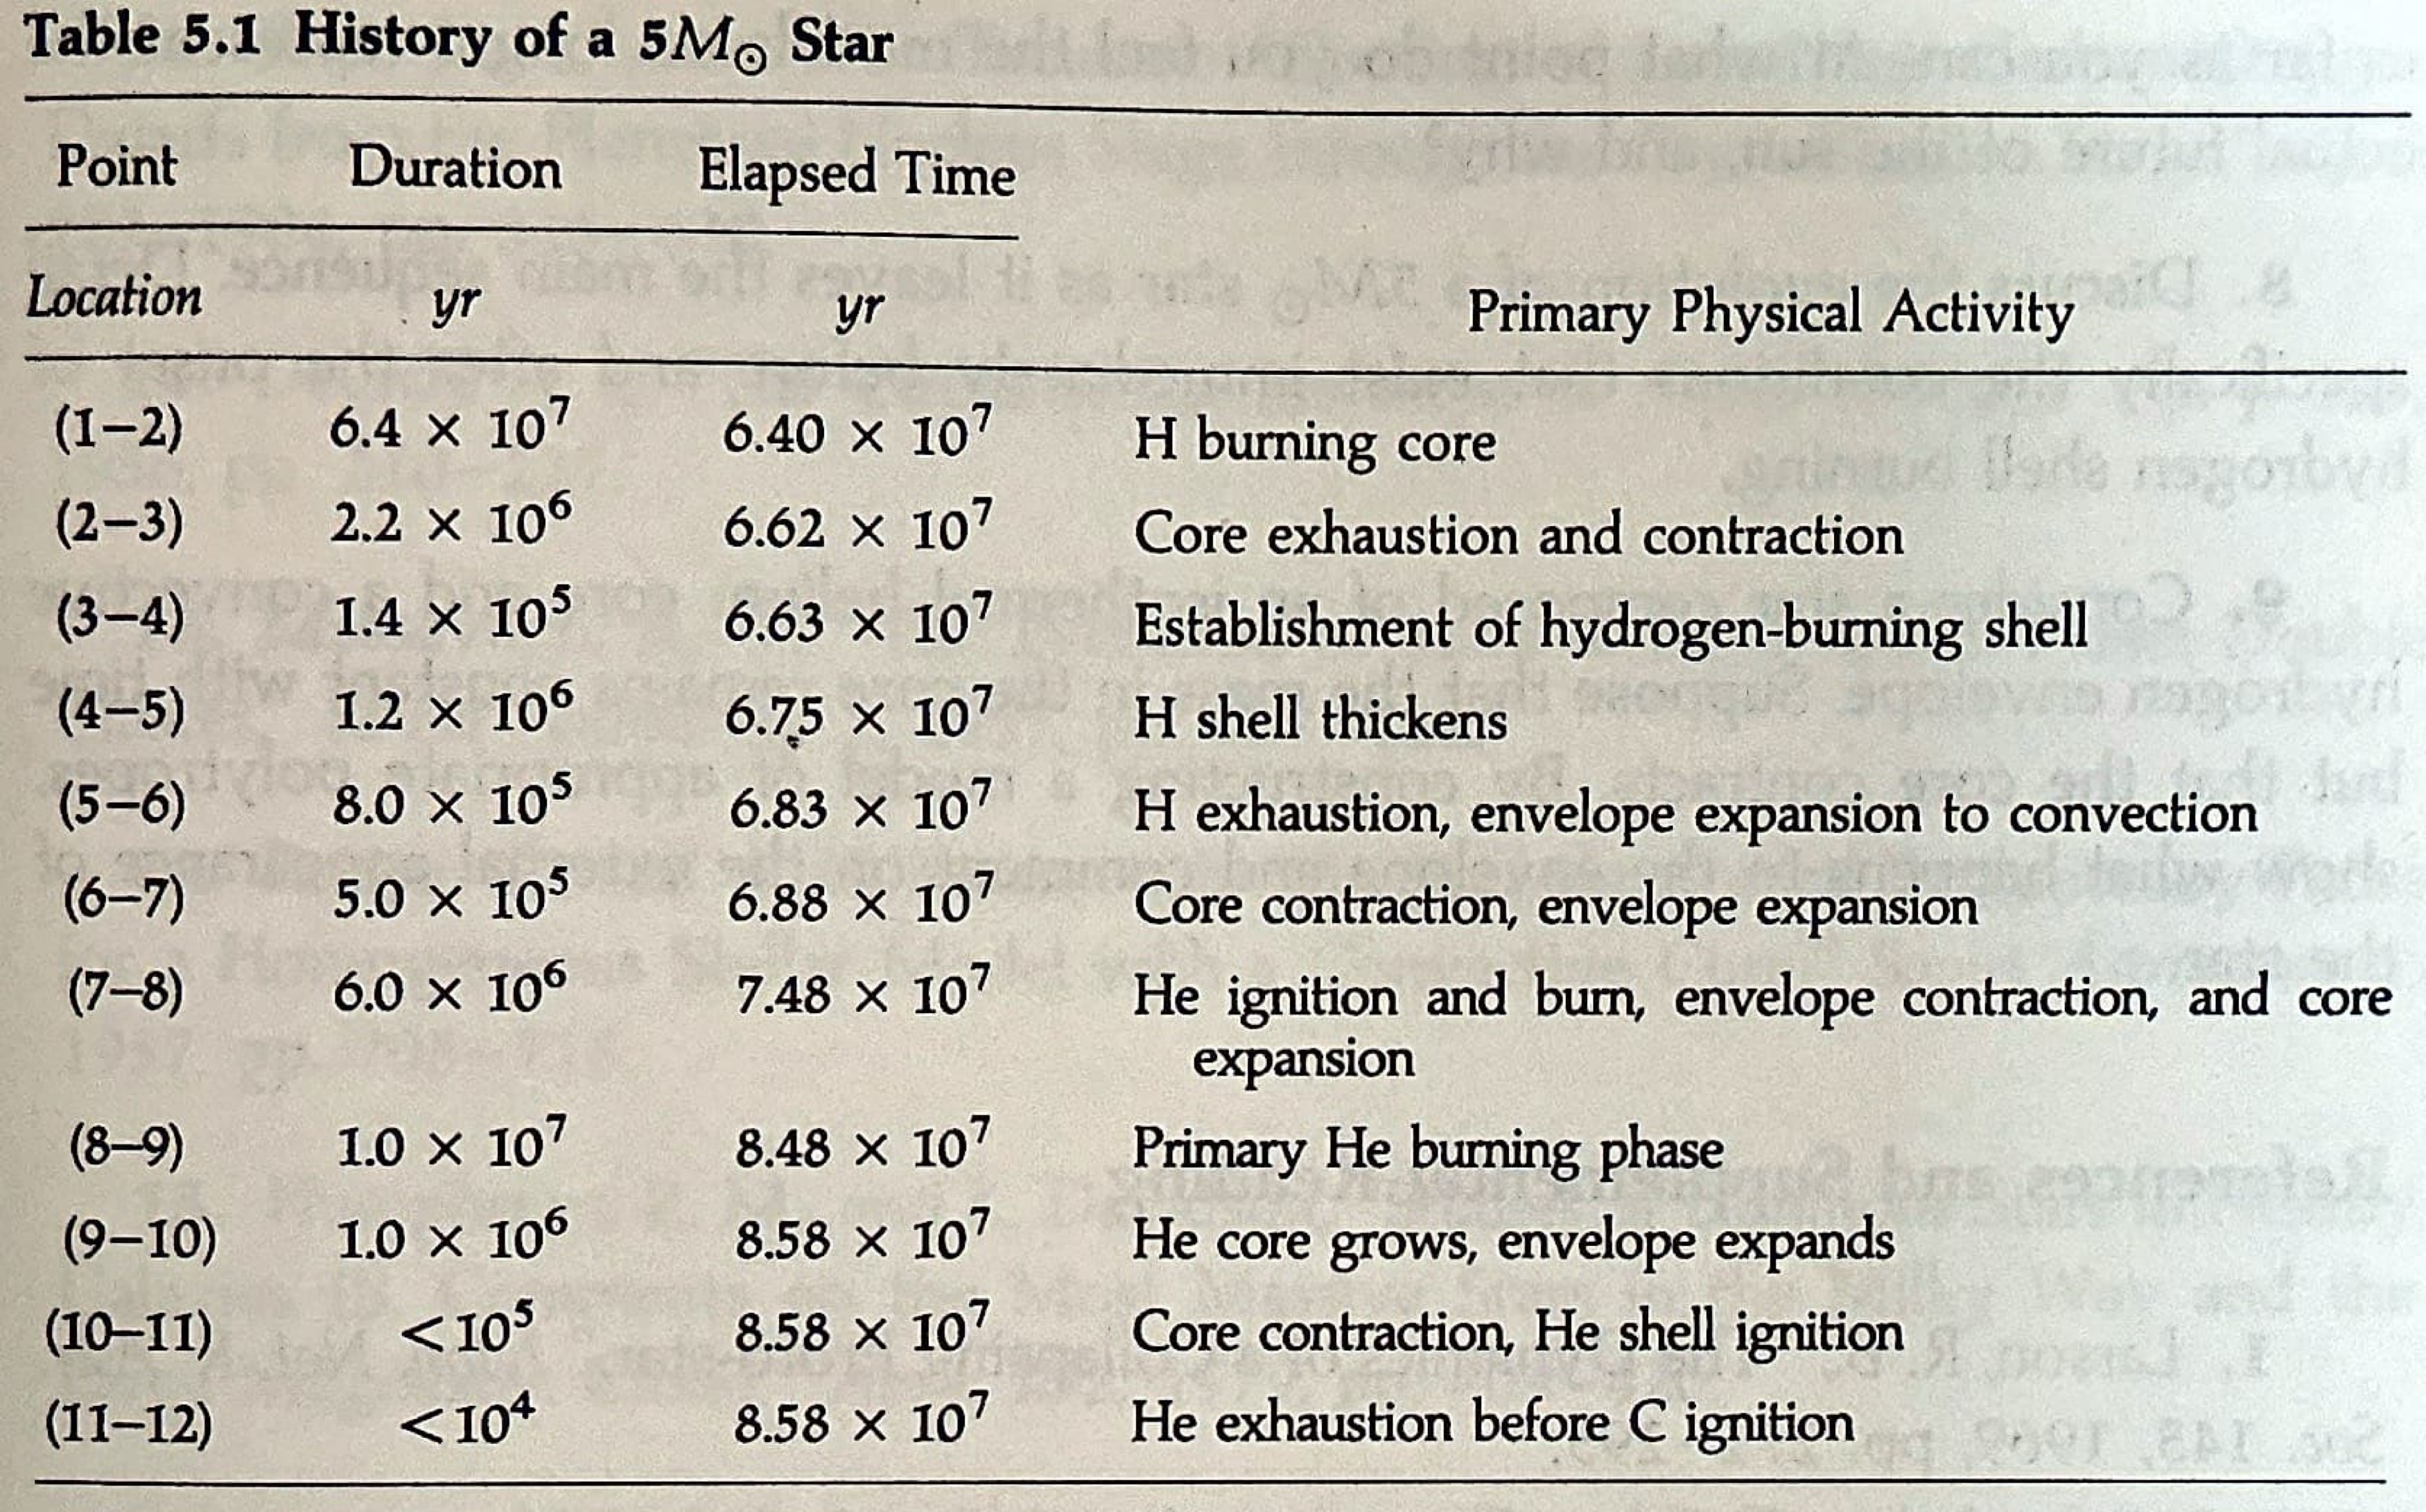
\includegraphics[trim={0cm 0cm 0 0},clip, keepaspectratio,width=0.95\textwidth,origin=c,angle=0]{5msun_tab}\label{fig:5msun_tab}
\end{figure}
        \end{column}
    \end{columns}
    
\end{frame}

\subsection{Deps of MS on Physical input}\linkdest{MSdeps}

\begin{frame}{Effects of changes in initial chemical composition}
\begin{block}{Different initial Y value: opacity and mean molecular weight}
\begin{columns}[T]
\begin{column}{0.5\textwidth}
\begin{figure}[!ht]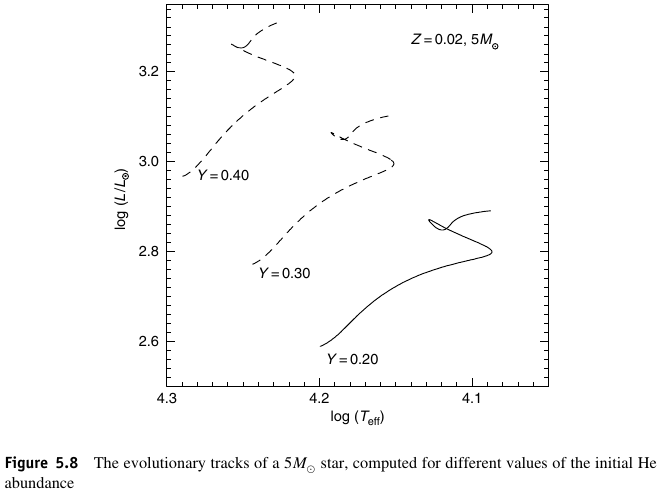
\includegraphics[trim={0cm 0cm 0 0},clip, keepaspectratio,width=0.99\textwidth]{HRD-changingHe}\label{fig:HRD-changingHe}
\end{figure}
\end{column}
\begin{column}{0.5\textwidth}
\begin{itemize}
    \item Increases of nuclear rates $L_H\propto\mu^7$
    \item Opacity decreases
\end{itemize}
Star is brighter and hotter
\end{column}
\end{columns}
\end{block}
\begin{block}{Changes in Z affect opacity}
\begin{itemize}
    \item \xaumenta{Z}, \xaumenta{\kappa}: fainter, cooler star.
    \item PP chain reaction not dependent on Z, CNO element are enough exept in pop III.
    \item $\alpha$-enhanced objects: CNO cycle efficiency increased, opacity increased with two bump at $\log{T}=6,5.5$ due to K shell O electrons and L-edges of Mg, Si, Ne. Stars are fainter and cooler
\end{itemize}
\end{block}
\end{frame}

\begin{frame}{Effects of changing convection efficiency: superadiabatic convection}
\begin{columns}[T]
\begin{column}{0.5\textwidth}
\begin{figure}[!ht]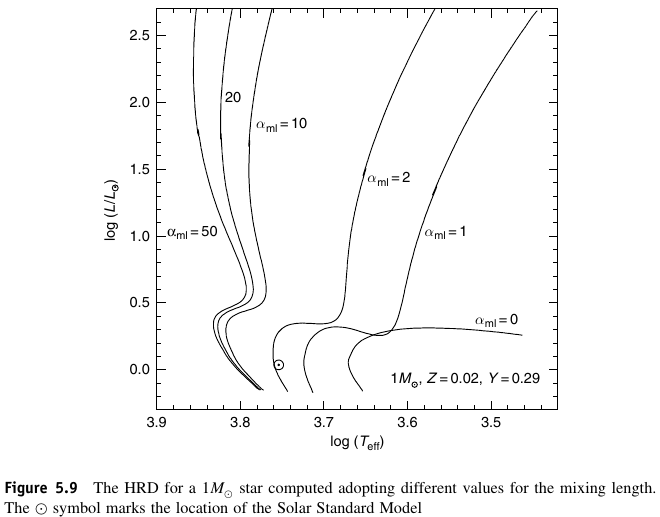
\includegraphics[trim={0cm 0cm 0 0},clip, keepaspectratio,width=0.99\textwidth]{HRD-1M-changingalpha}\label{fig:HRD-changingHe}
\end{figure}
\end{column}
\begin{column}{0.5\textwidth}
\begin{itemize}
    \item $\alpha_{ML}$ calibrated using Sun.
    \item $\alpha_{ML}$ does not affect L
    \item $\alpha_{ML}$ affects radius and $T_e$: \xaumenta{\alpha},\xdiminuisce{\nabla},\xaumenta{T_e},\xdiminuisce{R_s}
\end{itemize}
\end{column}
\end{columns}
\end{frame}

\begin{frame}{Convective core and Overshooting ($M>10\msun{}$)}
\begin{columns}[T]\begin{column}{0.5\textwidth}
\begin{figure}[!ht]
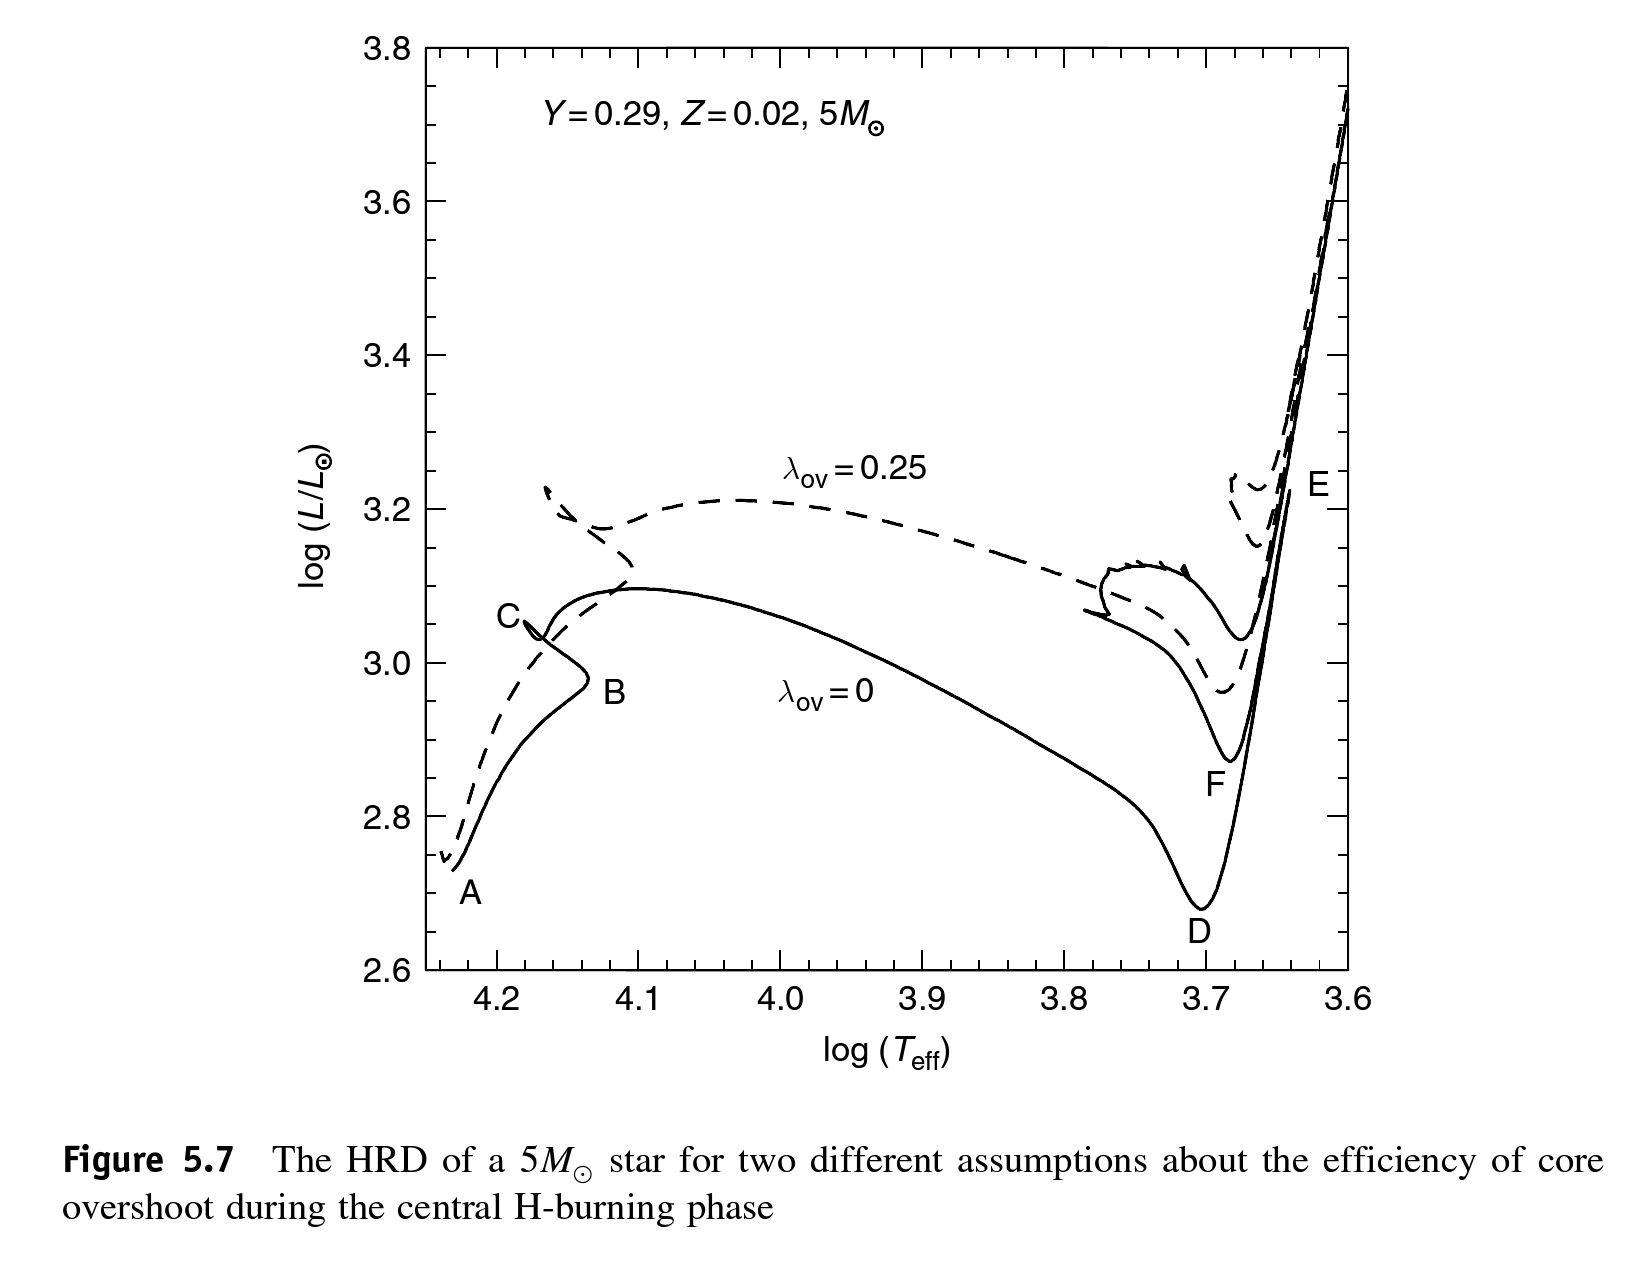
\includegraphics[trim={0cm 0cm 0 0},clip, keepaspectratio,height=0.42\textheight]{HRD-overshoot}\label{fig:HRD-overshoot}
\end{figure}
\end{column}
\begin{column}{0.5\textwidth}
\begin{block}{What increases convective core}
\begin{itemize}
\item Changes in physical input
\item Stellar rotation
\item Physical overshooting
\end{itemize}
\end{block}
\end{column}\end{columns}
\begin{columns}[T]\begin{column}{0.55\textwidth}
\begin{block}{Effects of increased convective core}
\begin{itemize}
\item \xaumenta{M_c}, \xaumenta{\mu} (involve more mass), \xaumenta{L}
\item Longer central H-burning
\item Larger He core at end of MS: brighter He-burning phase star, shorted lifetime
\end{itemize}
\end{block}
\end{column}
\begin{column}{0.45\textwidth}
\begin{block}{\sch vs Ledoux in-stability criterion}
In radiative region the retracting convective core leave chem composition gradient; but \xaumenta{He}, \xdiminuisce{\kappa}
\end{block}
\end{column}\end{columns}
\end{frame}

\begin{frame}{Low-mass star $M<0.4\msun{}$}
\begin{columns}[T]\begin{column}{0.45\textwidth}
\begin{figure}[!ht]
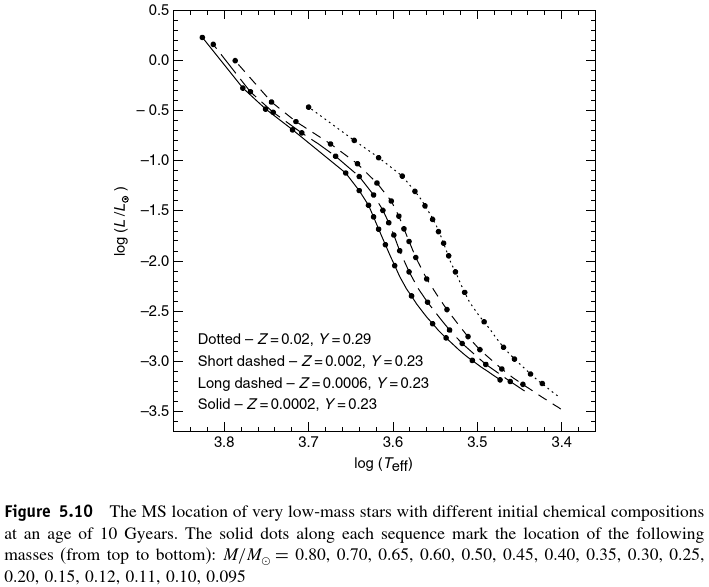
\includegraphics[trim={0cm 0cm 0 0},clip, keepaspectratio,width=0.99\textwidth]{VLM-HDR}\label{fig:VLM-HDR}
\end{figure}
\end{column}
\begin{column}{0.47\textwidth}
\begin{itemize}
    \item Fully convective through MS live
    \item PP1 H-burning with negligible $^3He$ destruction
    \item Transition between molecular H and atomic He to plasma at inner $90\%$ in mass: thermodynamical properties sensible to treatment of pressure ionizzation, dissociation, non-ideal Coulomb.
    \item Atmospheric features due to opacity sources: collisional induced dipole in $H_2$ molecules, CIA suppresses flux at \SI{2}{\micro\meter}; for $T_e<\SI{4000}{\kelvin}$ molecules of $TiO$ and $VO$ controll flux in optical, $H_2O$ and $CO$ the flux in infrared; for $T_e<\SI{2800}{\kelvin}$ also grains are important.
\end{itemize}
\end{column}\end{columns}
\end{frame}

\subsection{Mass-Luminosity relations: $L\propto M^3$}\linkdest{malure}

\begin{frame}{M-L relation}
\begin{columns}[T]\begin{column}{0.4\textwidth}
Near ZAMS $L\propto M^3$:
\begin{align*}
    &T^3\TDy{m_r}{T}=-\frac{3\kappa_R}{64\pi^2ac}\frac{L_r}{r^4}\Rightarrow L\propto \frac{R^4}{M}T_c^4\\
    &\TDy{m_r}{P}=-\frac{Gm_r}{4\pi r^4}\Rightarrow P\propto \frac{M^2}{R^4}\\
    &P\propto\rho T\propto \frac{M}{R^3}T\Rightarrow T_c\propto \frac{M}{R}
\end{align*}
\begin{figure}[!ht]
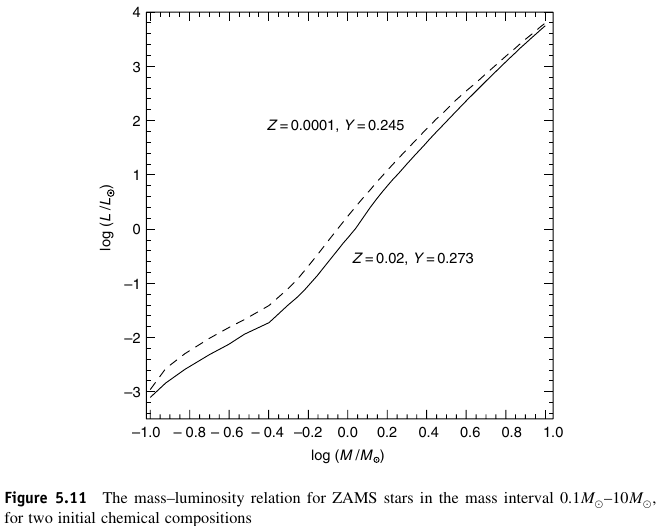
\includegraphics[trim={0cm 0cm 0 0},clip, keepaspectratio,width=0.99\textwidth]{ML-01-10}\label{fig:ML-01-10}
\end{figure}
\end{column}
\begin{column}{0.6\textwidth}
Scilla's Version:
\begin{align*}
    &\exv{\rho}\propto \frac{M}{R^3},\TDy{r}{P}=-\frac{\rho GM}{r^2}\Rightarrow \frac{P_e-P_c}{R-0}\propto-\frac{GM}{R^2}\frac{M}{R^3}\\
    &\Rightarrow P_c\propto\frac{M^2}{R^4},\ P\approx P_g=\frac{\rho}{\mu m_u}KT:\\
    &T_c\propto \frac{P_c\mu_c}{\rho_c}\propto \frac{P_c\exv{\mu}}{\exv{\rho}}\propto\frac{M^2}{R^4}\frac{R^3}{M}\exv{\mu}\Rightarrow T_c\propto \frac{M}{R}\exv{\mu}\\
    &\TDy{r}{T}|_{Rad}=-\frac{3}{4\pi ac}\frac{\exv{\kappa}\rho}{T^3}\frac{L(r)}{4\pi r^2}: L\propto-\frac{T^3}{\exv{\kappa}\rho}\TDy{r}{T}r^2\\
    &\Rightarrow L\propto \underbrace{\frac{M}{R^2}\mu}_{\TDy{r}{T}}\underbrace{\frac{M^3}{R^3}\exv{\mu}^3}_{T^3}\frac{1}{\exv{\kappa}}\underbrace{\frac{R^3}{M}}_{\frac{1}{\exv{\rho}}}R^2\propto \frac{\exv{\mu}^4M^3}{\exv{\kappa}}\tag{M-L relation}\\
    &\TDy{r}{L}=4\pi r^2\exv{\rho}\epsilon: \frac{L}{R^3}\propto\exv{\rho}\epsilon\Rightarrow\exv{\rho}\propto \frac{L}{R^3}\frac{1}{\epsilon}\\
    &T_c\propto \frac{M}{R}\Rightarrow R\propto \frac{M}{T}: \exv{\rho}\propto \frac{L}{M^3}\frac{T^3}{\epsilon}, L\propto M^3: \exv{\rho}\propto \frac{T^3}{\epsilon}\\
    &\epsilon\propto\rho^mT^n\tag{H fusion: $m=1$, PP: $n\approx4$, CN-NO: $n\approx\numrange{15}{17}$}\\
    &\Rightarrow\rho\propto \frac{T^3}{\rho^mT^n}: \rho^{m+1}\propto T^{3-n}\Rightarrow\rho^2\propto T^{3-n}
\end{align*}
    Relazione osservativa
\begin{equation*}
L\propto\begin{array}{l}
M\expy{3.6},\ \numrange{2}{20}\msun{}\\
M\expy{4.5},\ \numrange{0.5}{2}\msun{}\\
M\expy{2.6},\ \numrange{0.2}{0.5}\msun{}\\
\end{array}
\end{equation*}
For $M,\ M>10\msun{}$ relation becomes less steep $L\propto M$: due to increasing contribution of radiation pressure in massive stars.
\end{column}\end{columns}
\end{frame}

\subsection{Post-MS: SGB(const L, move Blue to Red), RGB (const T, L increases)}\linkdest{postMS}
%SC [160]

%\begin{frame}{Int-massive stars}
%\begin{figure}[!ht]
%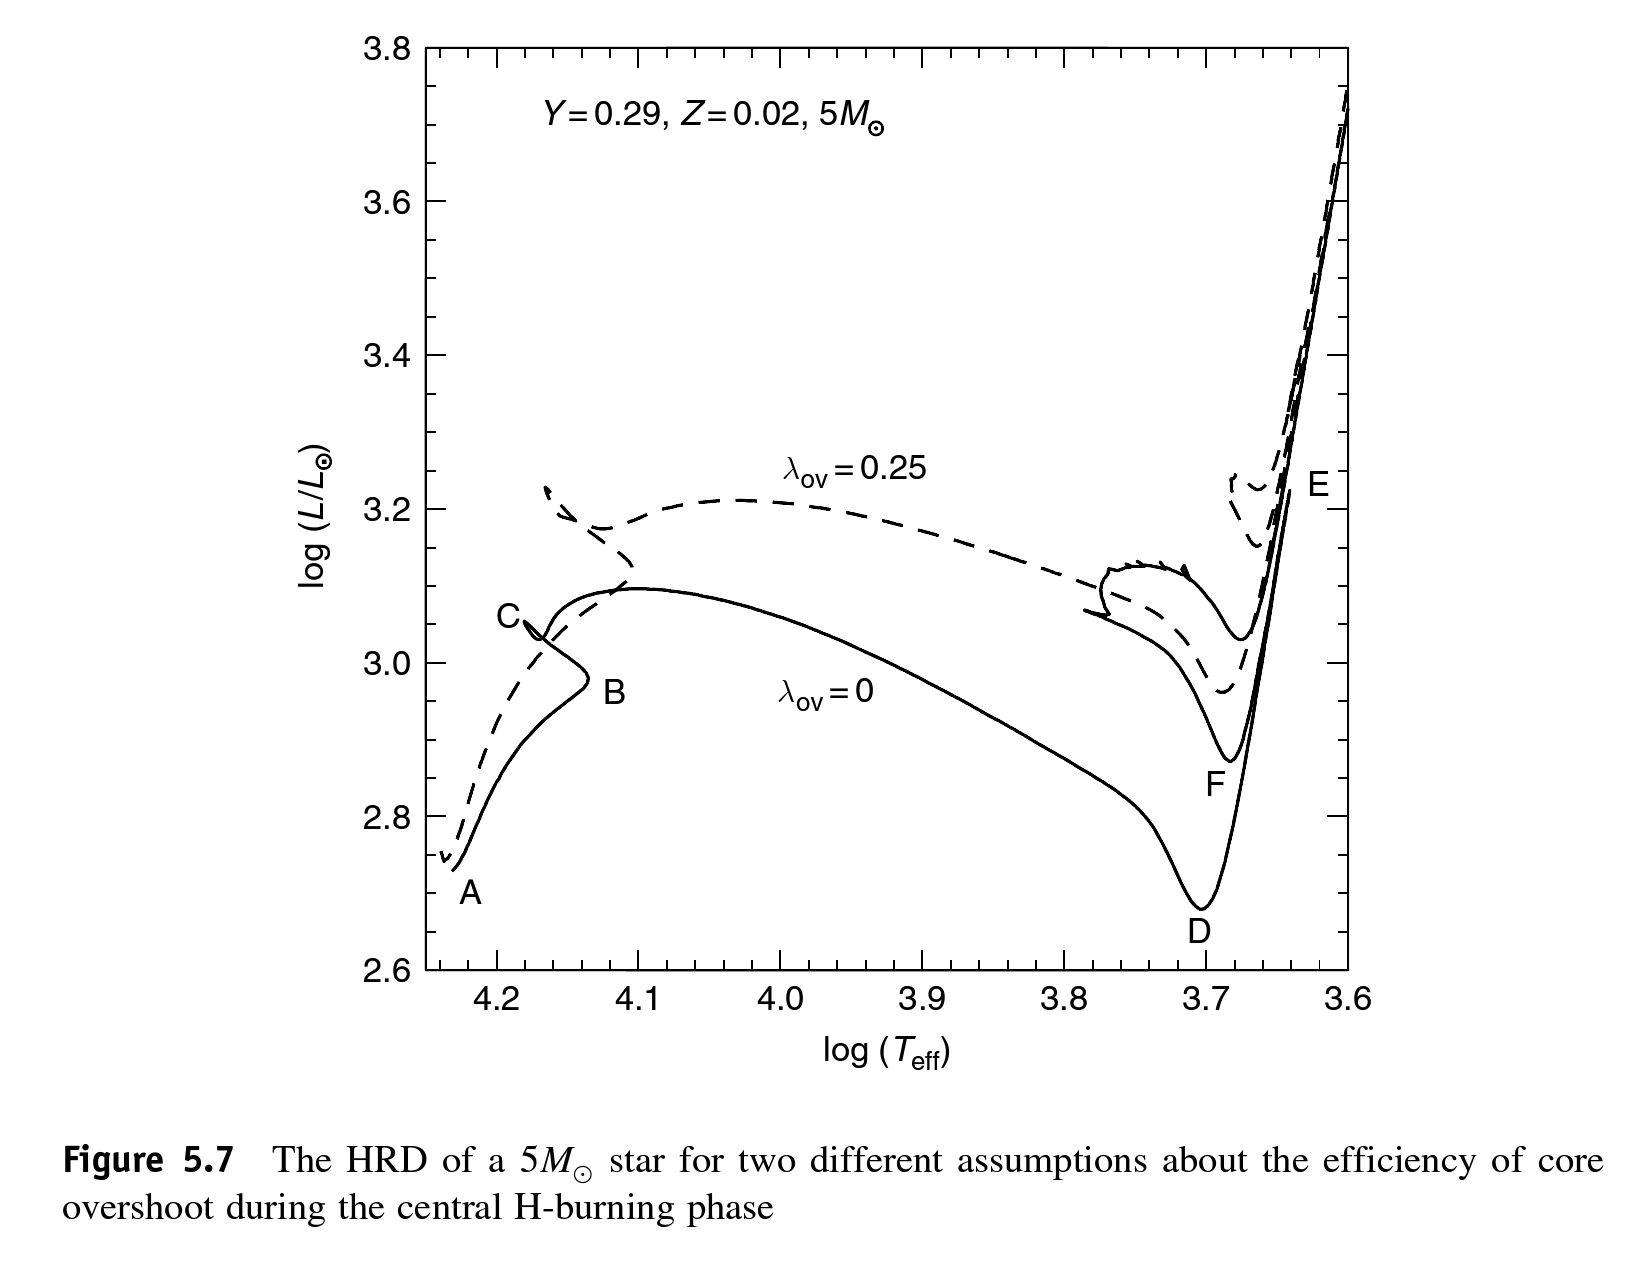
\includegraphics[trim={0cm 0cm 0 0},clip, keepaspectratio,height=0.42\textheight]{HRD-overshoot}\label{fig:HRD-overshoot}
%\end{figure}
%    \begin{itemize}
%        \item $M_{He,core}$ maggiore del limite SC
%        \item SGB: Structure move from blue to red side at almost constant surface L. $\tkh{}\approx\SI{12}{\mega\year}$ for $3\msun{}$, $\tkh{}\approx\SI{1}{\mega\year}$ for $6\msun{}$.
%        \item RGB: Point D - constant effective T while L increases; point E where He burning is efficient marks the end of RG phase.
%    \end{itemize}
%\end{frame}

\begin{frame}{Condizione Core per fusione: Virial theorem}
    \begin{columns}[T]
        \begin{column}{0.65\textwidth}
\begin{itemize}
    \item gravitational contraction: virial theorem
        \begin{align*}
            &\int_0^M\TDy{m}{P}4\pi r^3\,dm=-\int_0^M \frac{Gm}{r}\,dm\tag{HE$*4\pi r^3$}\\
            &\Rightarrow \underbrace{[4\pi r^3P]_0^M}_{P_{surf}\approx0,r=0}-\int_0^M12\pi r^2\TDy{m}{r}P\,dm=-\int_0^M \frac{Gm}{r}\,dm\\
            &E=\frac{3}{2}\frac{P}{\rho}\Rightarrow E=-\frac{\Omega}{2}\tag{Internal energy per unit mass: perfect monoatomic gas}\\
            &E_T=E+\Omega\Rightarrow E_T=-E, E_T=\frac{\Omega}{2}\\
            &L=-\TDy{t}{E_T}\Rightarrow L=-\frac{1}{2}\TDy{t}{\Omega}, \Delta E=-\Delta E_T=\frac{\Delta\Omega}{2}\tag{only grav}\\
            &E=\frac{1}{\gamma-1}\frac{P}{\rho}, \gamma=\frac{c_P}{c_v}(=\frac{5}{3}\text{perfect})\tag{generic perf. gas}\\
            &\Rightarrow E=-\frac{\Omega}{3(\gamma-1)},E_T=\frac{3\gamma-4}{3(\gamma-1)}\Omega\tag{Stability: HE $\gamma>\frac{4}{3}$}\\
            &3(\gamma-1)E+\Omega=4\pi R^3P_0\tag{Surf. press.}\\
        \end{align*}
\end{itemize}
        \end{column}
        \begin{column}{0.35\textwidth}
\begin{figure}[!ht] 
    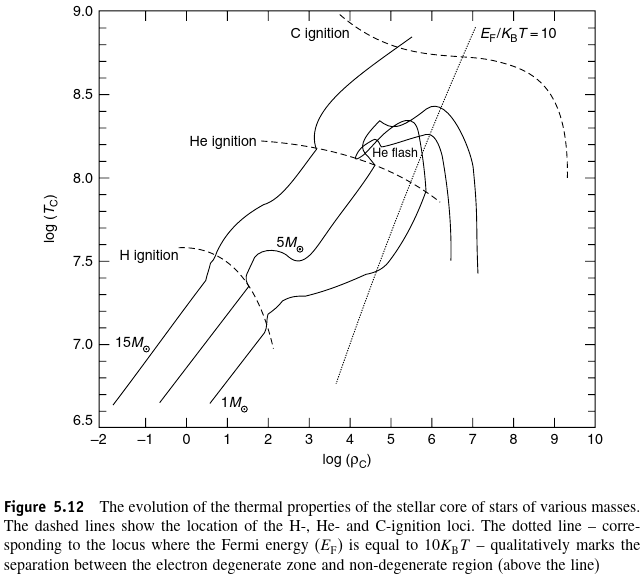
\includegraphics[trim={0cm 0cm 1cm 0cm},clip, keepaspectratio,height=0.3\textheight]{HHeCcore}\label{fig:HHeCcore}
\end{figure}
\begin{align*}
    &\Omega=-\alpha \frac{GM^2}{R}\\
    &\rho=\const:\alpha=\frac{3}{5}\\
    &E\approx \frac{3}{2}K\bar{T}\frac{M}{\mu m_H}\\
    &\Rightarrow\bar{T}\propto M^{\frac{2}{3}}\bar{\rho}^{-\frac{1}{3}}
\end{align*}
        \end{column}
    \end{columns}
\end{frame}

\begin{frame}{Condizione Core per fusione: virial theorem and degenerate electrons}
    \begin{itemize}
        \item Electron degeneracy: $3(\gamma-1)$ is 2 (NR) or 1 (R) for degenerate \Pelectron; for mixture \Pelectron-ions $\gamma>\frac{4}{3}$. Case NR \Pelectron deg. $3(\gamma-1)=2$  (NR: $\gamma=\frac{5}{3}$): $\Omega=-2E=2E_{Tot}$, if $L=-\frac{1}{2}\TDy{t}{\Omega}$, $\Omega\propto \frac{1}{R}\propto\rho^{\frac{1}{3}}$ implica $\frac{1}{\Omega}\TDy{t}{\Omega}=\frac{1}{3}\frac{1}{\rho}\TDy{t}{\rho}$     
            \begin{align*}
                &n_e=\frac{\rho}{\mu_em_H}=\frac{8\pi p_F^3}{3h^3}\Rightarrow\rho\propto E_F^{\frac{3}{2}}\\
                &E=\int_0^{E_F}n(E_{kin}\,dE_{kin}=\frac{1}{\rho}\int_0^{E_F}\frac{8\sqrt{2}\pi m_e^{\frac{3}{2}}}{h^3}E_{kin}^{\frac{3}{2}}\,dE_{kin}\propto \frac{1}{\rho}E_F^{\frac{5}{2}}\propto \frac{\rho^{\frac{5}{3}}}{\rho}\propto\rho^{\frac{2}{3}}\tag{Internal Energy}\\
                &\Rightarrow \frac{1}{E_e}\TDy{t}{E_e}=\frac{2}{3}\frac{1}{\rho}\TDy{t}{\rho}\Rightarrow\TDy{t}{E_e}\approx2 \frac{E_e}{\Omega}\TDy{t}{\Omega}\\
        &\Omega=-2E, E=E_I+E_E\Rightarrow \Omega\approx-2E_e\tag{High degeneracy}\\
        &\TDy{t}{E_e}\approx2 \frac{E_e}{\Omega}\TDy{t}{\Omega}\Rightarrow\TDy{t}{E_e}\approx-\TDy{t}{\Omega}\\
        &L=-\TDy{t}{E_{tot}}=-\TDy{t}{E_e}-\TDy{t}{E_i}-\TDy{t}{\Omega}\approx-\TDy{t}{E_i}
            \end{align*}
    \end{itemize}
    Half gravitational energy not radiated away increases electron internal energy (Fermi energy), whereas ions thermal energy decreases. Evolution of degenerate object (WD) can be considered at constant radius $\Delta\Omega=\frac{\Delta R}{R^2}\approx L$
\end{frame}

\begin{frame}{SC-mass limit: upper limit to $M_c/M_{tot}$} 
$\epsilon_n=0$ e gradiente radiativo implica formazione core di He isotermo: se la massa del core di elio \'e maggiore del $10\%$ della massa totale della stella il core si contrae - le stelle della LMS hanno core pi\'u piccolo, stelle di massa $M\geq2.5-3\msun{}$  hanno core pi\'u grande.
\begin{equation*} 
\frac{M_c}{M}>(\frac{M_c}{M})_{SC}=0.37(\frac{\mu_{env}}{\mu_c})^2\xrightarrow{\parbox{2.5cm}{$\mu_e=\mu_{\odot}=0.6$\\$\mu_c=\mu(He)=1.3$}}0.08
\end{equation*}
il core si contrae su $\tkh{}$.
Virial theorem for non-vanishing pressure surface pressure $P_0$ and $M_c$, $R_c$ and $T_c$:
\begin{align*}  
&(2U_i+\Omega+S_p=0,\ S_p=-\int\exv{v^2}\Vec{r}\cdot\hat{n}\,dS=P_0V)\\
&P_0=K_1\frac{M_cT_c}{R_c^3}-K_2\frac{M_c^2}{R_c^4}\tag{first term comes from Tot internal energy of core, second from grav. pot.}\\
&\frac{3}{2}\frac{K}{\mu m_u}T_cM\tag{total internal energy of core}\\
&P_{0,m}=K_3T_c^4/M_c^2
\end{align*}
For equilibrium $P_{0,m}\geq P_e\propto M_t^2/R^4=T_c^4/M_t^2$ ($T_c\propto M_t/R$)
\end{frame}

\subsection{Intermediate, massive stars: He-ignition in non degenerate core ($M>2.3\msun{}$)}

\begin{frame}{Int-massive($M_*>2.3\msun{}$) stars: from SG to RG}
\begin{columns}[T]\begin{column}{0.5\textwidth}
\begin{figure}[!ht]
%trim: LBRT
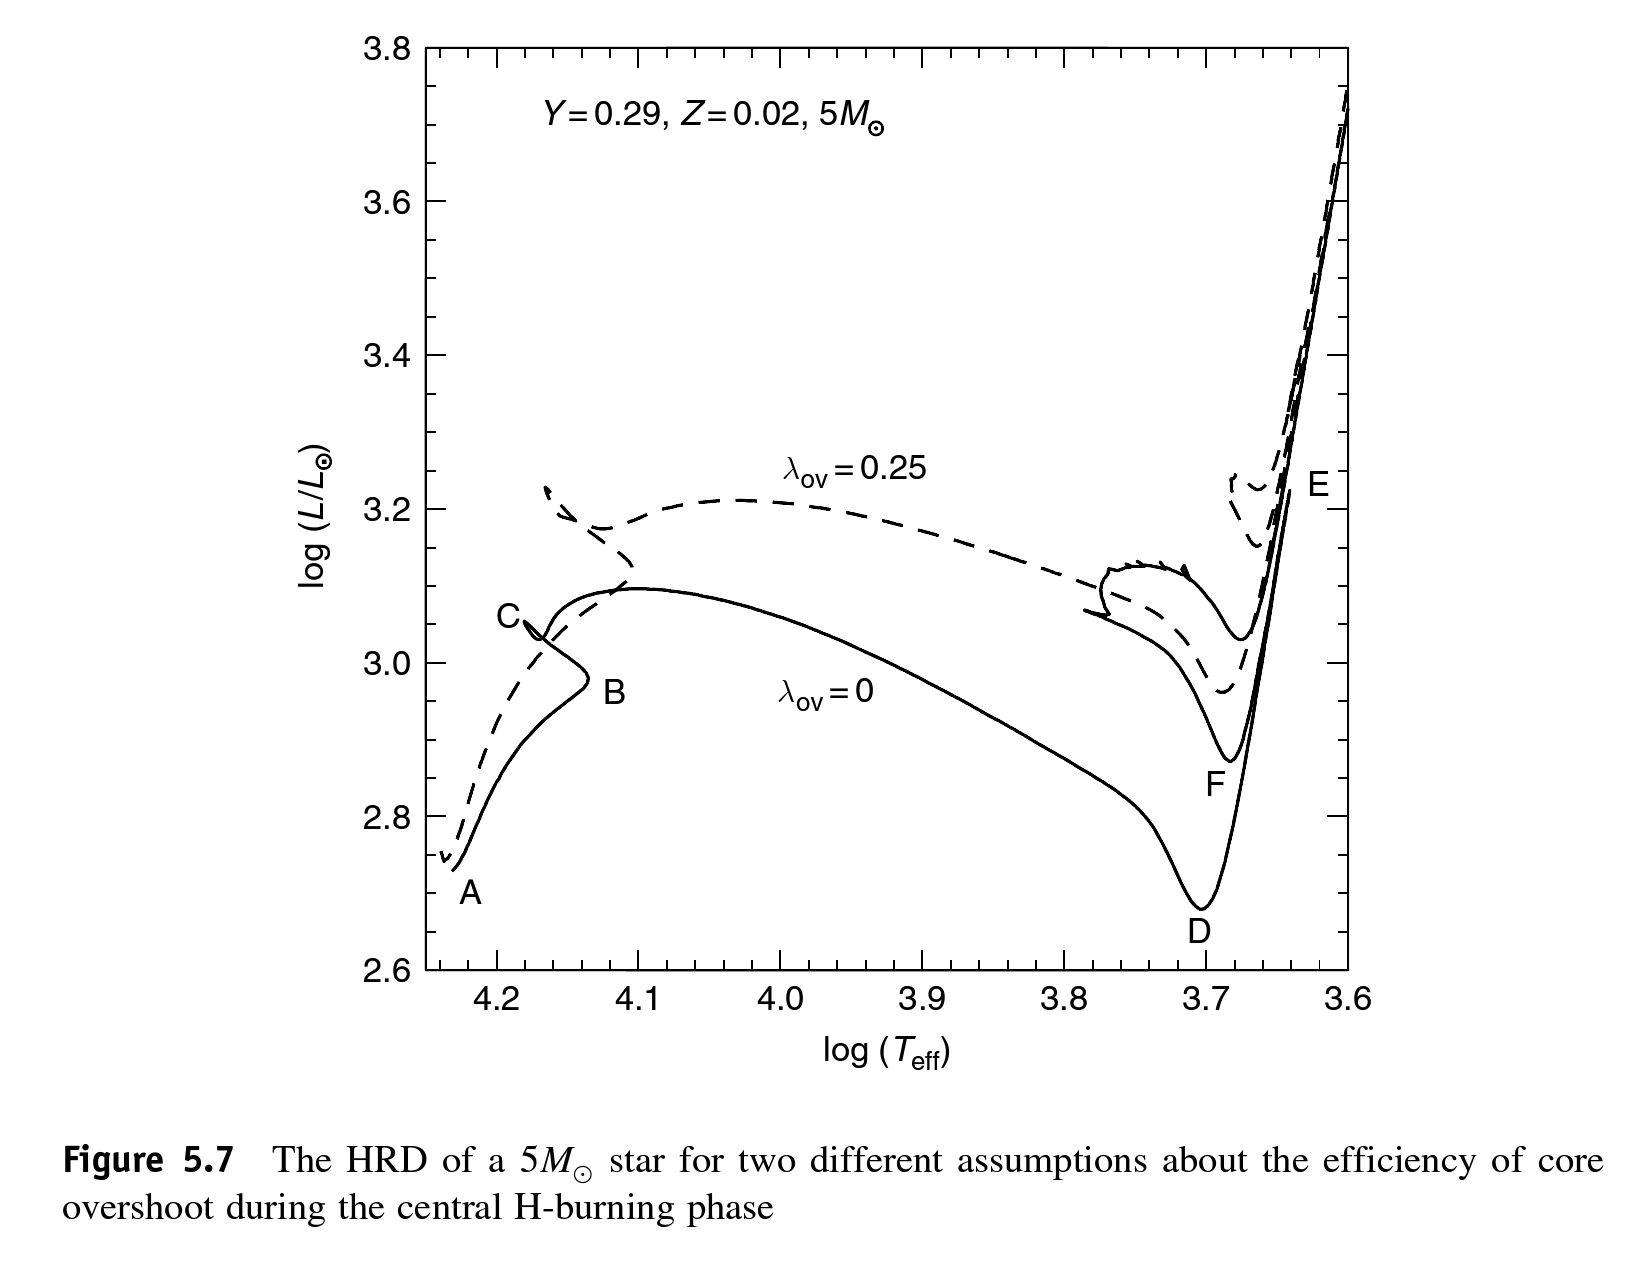
\includegraphics[trim={2.5cm 2cm 3.5cm 2.5cm},clip, keepaspectratio,width=0.99\textwidth]{HRD-overshoot}\label{fig:HRD-overshoot}
\end{figure}
\end{column}
\begin{column}{0.45\textwidth}
\begin{itemize}
    \item $M_c>M_{SC}$ (per $M\approx2.3-3$ limite superato dopo H-burning in shell): He core contract
    \item broad shell of CNO H-burning: $\epsilon_g$ changes sign at max $\epsilon_{CNO}$ - envelope expand: \xdiminuisce{T_e}, \xaumenta{\kappa_e} quindi inviluppo diventa convettivo.
    \item Star move from B to R at constant L - Hertzsprung gap: $\begin{array}{c}\tkh{}(3\msun{})\approx\SI{12}{\mega\year}\\\tkh{}(6\msun{})\approx\SI{1}{\mega\year}\end{array}$
\end{itemize}
\end{column}\end{columns}
\begin{itemize}
    \item In (D) star reaches Hayashi track where begins RG phase: $T_e$ costante, \xaumenta{L}. In (D) the stellar envelope becomes convective as it has cooled down during expansion: since it very efficient energy transport mechanism prevent slow down expansion.
    \item $\rho_c$ suff. low such onset of \Pelectron degeneracy is avoided: in (E) contracting core reaches $T\approx\SI{e8}{\kelvin}$ for efficient He-burning. \xaumenta{M_c} (VT: \xaumenta{T_c}) \xdiminuisce{\tau_{RG}}
\end{itemize}
\end{frame}

\subsection{Low-mass stars: He-flash and Dredge-up. Radiative core convective envelope.}

\begin{frame}{Low-mass stars}
    \begin{itemize}
        \item $M_{He,core}$ below SC limit and even when H-burning in shell produce bigger He-core the electron degeneracy provide support against contraction.
        \item $M_{cHe}-L$ relation: L provided by H-burning shell whose thermal prop are determined by He-core radius and mass.
        \item If evolving  at constant mass, Lower mass RGB stars at given L have larger radii and lower $T_{eff}$: mass loss shift star $T_e$ toward lower values.
        \item First dredge-up: as \xdiminuisce{T_e} during envelope expansion the convection goes deeper; Surface abundance of He monotonically increses as convection goes deeper; also $^3He$ and CNO elements are mixed.
        \item RGB bump: along RGB convection receeds as H-burning shell moves outward and when H-burning shell encounter discontinuity have peculiar behaviour in that region of HRD (\xaumenta{X},\xdiminuisce{T},\xdiminuisce{L})- stars stay $20\%$ of RGB lifetime in region of HRD.
        \item Max T moves outside center in He core
        \item He ignited when $M_{cHe}\approx0.5\msun{}$ in shell around degenerate core.
        \item Thermal runaway at Tip of RGB: He-flash.
    \end{itemize}
\end{frame}

%trim: LBRT
\begin{frame} {Low-mass stars: nuclear burning changing after X exhaustion in the center}
\begin{columns}[T]\begin{column}{0.5\textwidth}
\begin{figure}[!ht]
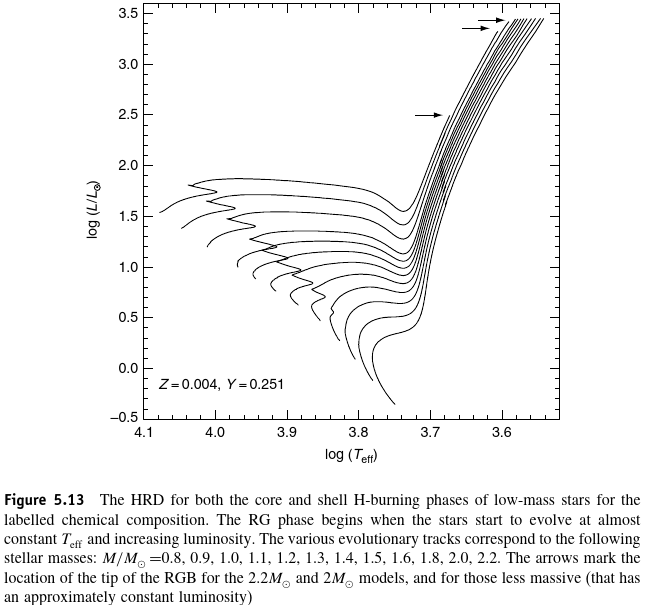
\includegraphics[trim={0cm 0cm 0cm 0cm},clip, keepaspectratio,width=0.99\textwidth]{HDRtipRGB}\label{fig:HDRtipRGB}
\end{figure}
\end{column}
\begin{column}{0.4\textwidth}
\begin{itemize}
\item As X exhausts max $\epsilon_H$ is no more in central region (at TO at $M_r=0.1\msun{}$). He Core (radiative/small convective??): $M<M_{SC}$, high electron degeneracy.
\item From TO to RG H-burning shell becomes thinner due to CNO deps on T that decreses in envelop and to X exhaustion.
\end{itemize}
\end{column}\end{columns}
\begin{itemize}
\item $M_{cHe}-L$ relation: \xaumenta{M_{cHe}}, \xaumenta{L}. L is almost fully provided by H-burning shell whose thermal properties are determined $R_c$, $M_c$ ($P_e$ is OM lower)
%\item RGB stars evolve at constant L and radius re-adjust to stellar mass: mass loss shift $T_e$ toward lower values.
\end{itemize}
\end{frame}

\begin{frame}{Envelope structure: depth of convection and first dredge-up}
\begin{columns}[T]\begin{column}{0.44\textwidth}
%trim: LBRT
\begin{figure}[!ht] 
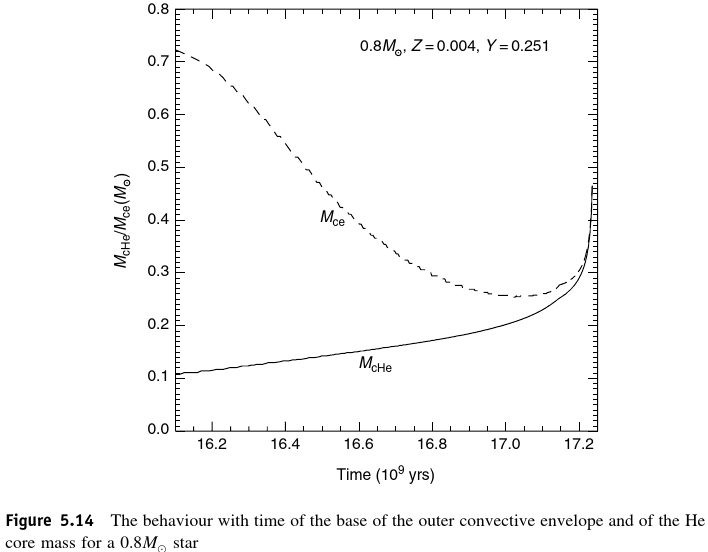
\includegraphics[trim={0cm 0cm 1cm 0cm},clip, keepaspectratio,height=0.42\textheight]{postMS-depthC}\label{fig:postMS-depthC}
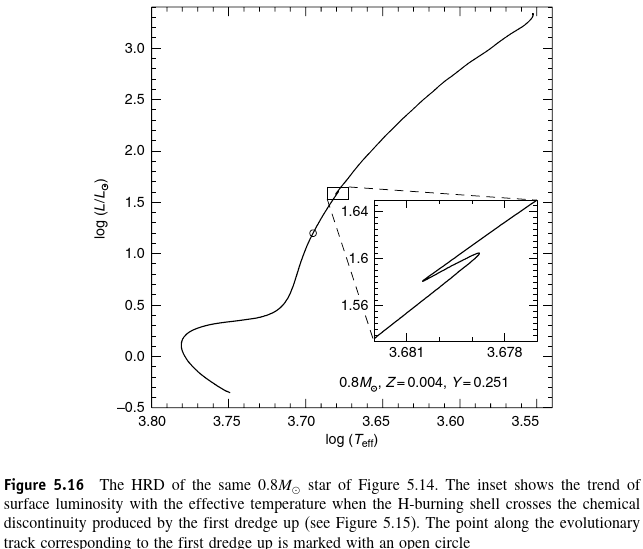
\includegraphics[trim={0cm 0cm 1cm 0cm},clip, keepaspectratio,height=0.42\textheight]{HburnxIdu}\label{fig:HburnxIdu}
\end{figure}
\end{column}
\begin{column}{0.50\textwidth}
\begin{itemize}
\item Cooling  of envelop causes deeper convection that reaches a maximum before RG (\xdiminuisce{T}, \xaumenta{\kappa}). Primo dredge-up: \xaumenta{He_s}, \xaumenta{^{14}N_s}, \xdiminuisce{^{12}C} ($\frac{^{12}C}{^{13}C}$), $Li$, $Be$ reduces several OM.
\item In  RGB phase H-burning shell move outward and convective zone move toward surface: chemical discontinuity at max convective depth. \keyword{Bump of RGB}: as H-burning shell meet discontinuity $L_H\propto\mu^7$ diminish the in fully mixed envelop \xaumenta{L} as \xaumenta{M_{cHe}} - bump in RGB luminosity function ($20\%$ rgb-time in this luminosity range)
\end{itemize}


\begin{figure}[!ht] 
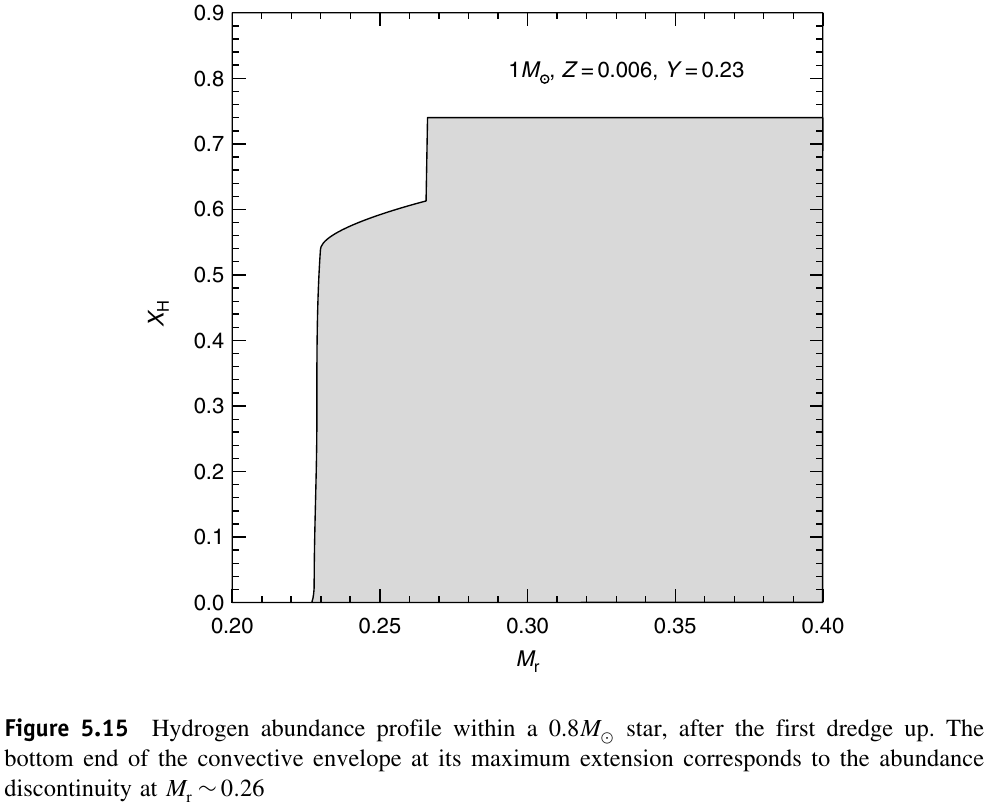
\includegraphics[trim={0cm 0cm 1cm 0cm},clip, keepaspectratio,height=0.35\textheight]{dredgedup-X}\label{fig:dredgedup-X}
\end{figure}
\end{column}\end{columns}
\end{frame}

\begin{frame}{\keyword{Thermal runaway at tip of RGB}: He-flashes}
\begin{columns}[T]\begin{column}{0.48\textwidth}
%trim: LBRT
\begin{figure}[!ht]
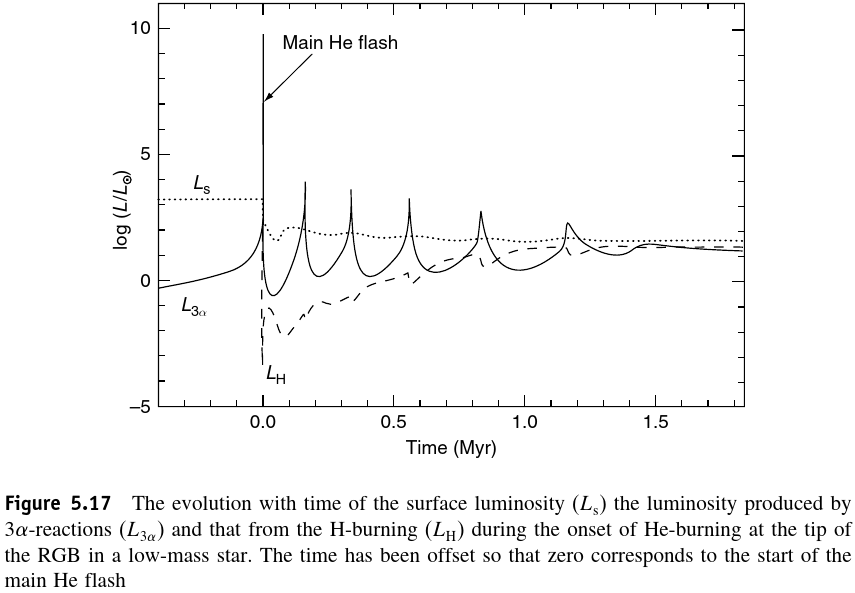
\includegraphics[trim={0cm 0cm 1cm 0cm},clip, keepaspectratio,width=0.99\textwidth]{He-flash}\label{fig:He-flash}
\end{figure}
\end{column}
\begin{column}{0.43\textwidth}
    In RG phase: H-burning increases $M_{cHe}$ and \xaumenta{\rho_c}. In inner part $M_r<0.3M_t$ when $\epsilon_g+\epsilon_{\nu}<0$: $\TDy{r}{L}<0$ resulting in T-inversion. \xaumenta{\rho_c}, grado di degenerazione aumenta, \xdiminuisce{\kappa_{cond}}, \xdiminuisce{T_c} (strong degeneracy: $\kappa_{cd}\propto\rho^{-2}T^2$); while \xaumenta{T_c^M} due to $\epsilon_g>0$ at boundary between D/ND matter. At $T_c^M\approx\SI{e8}{\kelvin}$ we have He ignition ($M_{cHe}\approx0.48-0.5\msun{}$): end of RGB phase.
\end{column}\end{columns}
He ignition at strong partial-relativistic-D ($\rho_x\approx\SI{e6}{\gram\per\cubic\cm}$, $T\approx\SI{8e7}{\kelvin}$), $P$ is insensitive to $T$ changes, rate of $3\alpha$-burning increases much: thermal runaway $\num{e10}\lsun{}$ in few seconds are absorbed by above ND layers: expansion and convection (large jump in P/S prevent mixing with above H-burning). So \xaumenta{T} at constant $\rho$ but no time for heat diffuse the whole core: this need many successive He-flashes, $\tau_{flash}\approx\SI{e6}{\year}$ and $5\%$ He converted to C
\end{frame}

\begin{wordonframe}{SC: WD cooling $[22], [45]$, Z poor $[196]$}

\end{wordonframe}

\subsection{Deps of RGB on params}\linkdest{depsRGB}

\begin{frame}{Location of RGB on HRD}
\begin{itemize}
\item Highly Z-dependent: size of convective envelop (Hayashy track) \xaumenta{Z}, \xaumenta{\kappa}, inviluppo convettivo pi\'u grande:  $\alpha$-enhanced stars (more low ionization potential: Mg, Si, ...) form molecule $TiO$ and $H^-$: RGB cooler and less steeper.
\item \xaumenta{Y}, \xdiminuisce{\kappa}, \xdiminuisce{CE}, \xaumenta{T_e}
\item RGB is important Z indicator of galaxies/star clusters
\item $\rho_e$ low: $\nabla_e$ \'e super-adiabatico (\xaumenta{
\alpha_{ML}},\xaumenta{T_e})
\item \keyword{RGB phase transition}. \xdiminuisce{M_*}, \xdiminuisce{T_e}: $M_{cHe}$ constant for $M\leq1.8\msun{}$ then decreases with $M$ as degeneracy is completely removed 
\end{itemize}
\end{frame}

\begin{frame}{Deps RGB's L-bump on params}
\begin{columns}[T]\begin{column}{0.52\textwidth}
%trim: LBRT
\begin{figure}[!ht]
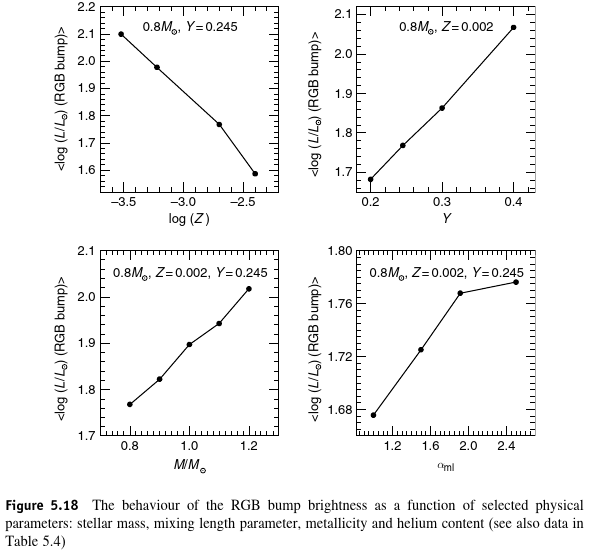
\includegraphics[trim={0cm 0cm 1cm 0cm},clip, keepaspectratio,width=0.99\textwidth]{RGB-bumpparams}\label{fig:RGB-bumpparams}
\end{figure}
\end{column}
\begin{column}{0.43\textwidth}
As convection zone goes deeper the H-burning shell takes less time to cross chemical discontinuity: (\xdiminuisce{M_*}/\xaumenta{Z}/\xdiminuisce{Y},\xdiminuisce{\alpha_{ML}}), \xdiminuisce{L_{bump}}
\end{column}\end{columns}
\end{frame}

\begin{frame}{Deps RGB tip's (He-ignition) luminosity on params}
\begin{columns}[T]\begin{column}{0.5\textwidth}
%trim: LBRT
\begin{figure}[!ht]
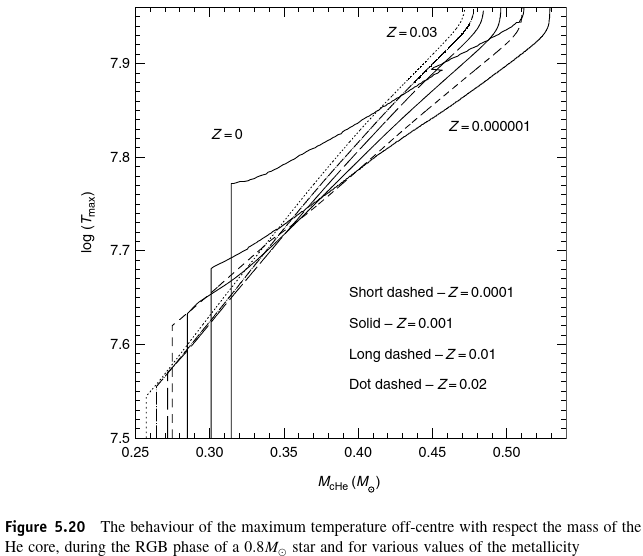
\includegraphics[trim={0cm 0cm 1cm 0cm},clip, keepaspectratio,height=0.36\textheight]{RGBTmax}\label{fig:RGBTmax}
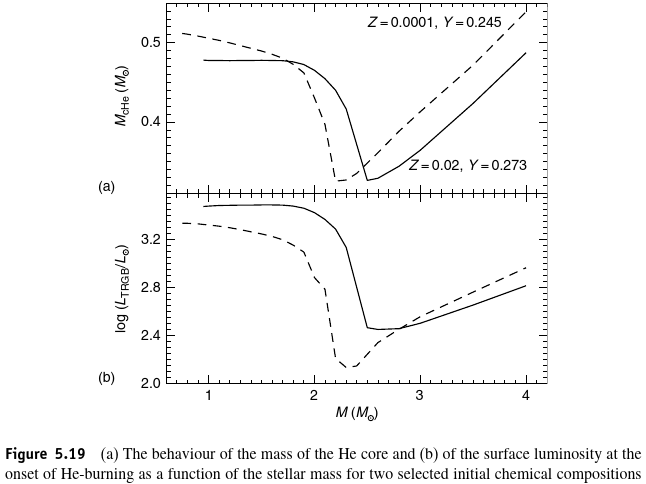
\includegraphics[trim={0cm 0cm 1cm 0cm},clip, keepaspectratio,height=0.36\textheight]{HecLsatHeburning}\label{fig:HecLsatHeburning}
\end{figure}
\end{column}
\begin{column}{0.45\textwidth}
\begin{itemize}
    \item \keyword{RGB phase transition}. \xdiminuisce{M_*}, \xdiminuisce{T_e}: $M_{cHe}$ constant for $M\leq1.8\msun{}$ then decreases with $M$ as degeneracy is completely removed then increases as consequences of larger convective H-burning core.
    \item \xaumenta{He}, \xaumenta{T_c}, deg \Pelectron diminuisce, $M_{cHe}$ He-ignition diminuisce, \xdiminuisce{L_{TIP}}
    \item \xaumenta{Z}, \xaumenta{\epsilon_{CNO}}, $M_{cHe}$-ignition is builded faster since He production is faster and He-core heating is faster, \xaumenta{L_{TIP}}
\end{itemize}
\end{column}\end{columns}
\end{frame}

\subsection{Very low Z stars}\linkdest{lowz}

\begin{frame}{Very low Z (pop III)}
\begin{itemize}
    \item Primordial star (Pop III) responsable for Z-enrichment: from $Z\approx\numrange{e-10}{e-12}$ to $Z\approx\numrange{e-2}{e-3}$ (Pop II)
    \item High mass star burn H through PP chain so need much higher T; as $T\approx\SI{e8}{\kelvin}$ He-burning produce $^{12}C$: threshold for CNO H-burning to begins $X_C\approx\numrange{e-9}{e-10}$
    \item \xaumenta{M_*}, \xdiminuisce{\tau_{PP\to CNO}}: transition to convective core for $M>2\msun{}$ (for $M=2-5\msun{}$ convective core after $^3He$ production phase).
    \item RGB phase transition at lower mass/higher age: for low mass star \xaumenta{T_c} due to low, degenerazione elettronica del core di He diminuisce, faster He ignition, \xdiminuisce{M_{cHe}}, \xdiminuisce{L_{TIP}}
    \item Intermediate mass star have no RGB
\end{itemize}
\begin{columns}[T]
    \begin{column}{0.5\textwidth}
        \begin{figure}[!ht] 
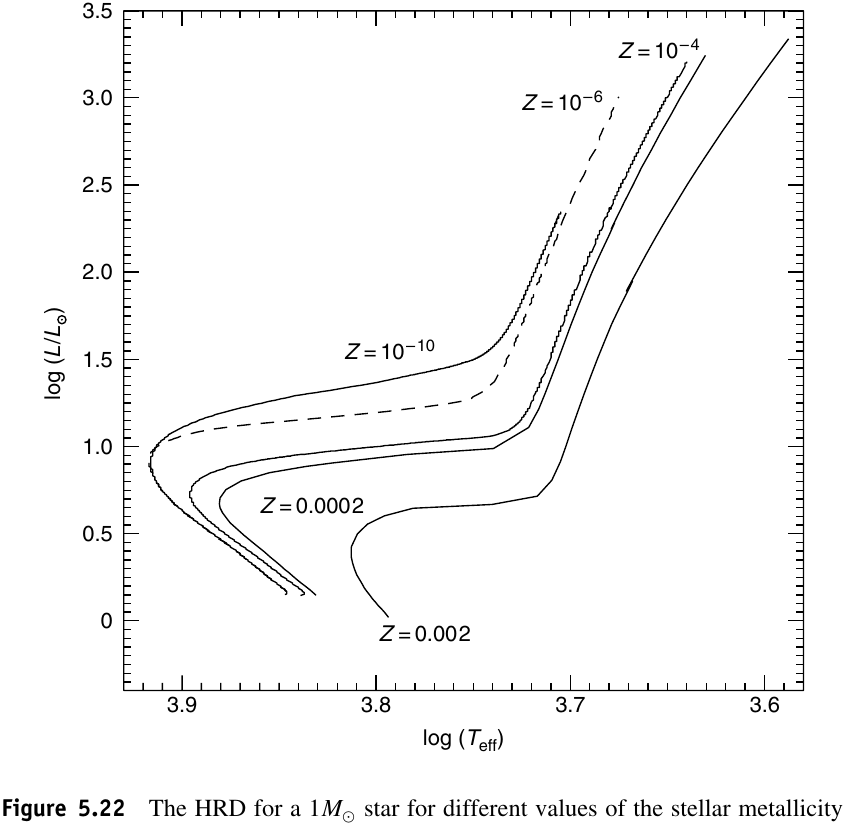
\includegraphics[trim={0cm 0cm 0cm 0cm},clip, keepaspectratio,width=0.85\textwidth]{lowZ1MsunHDR}\label{fig:lowZ1MsunHDR}
\end{figure}
    \end{column}
    \begin{column}{0.5\textwidth}
        \begin{figure}[!ht] 
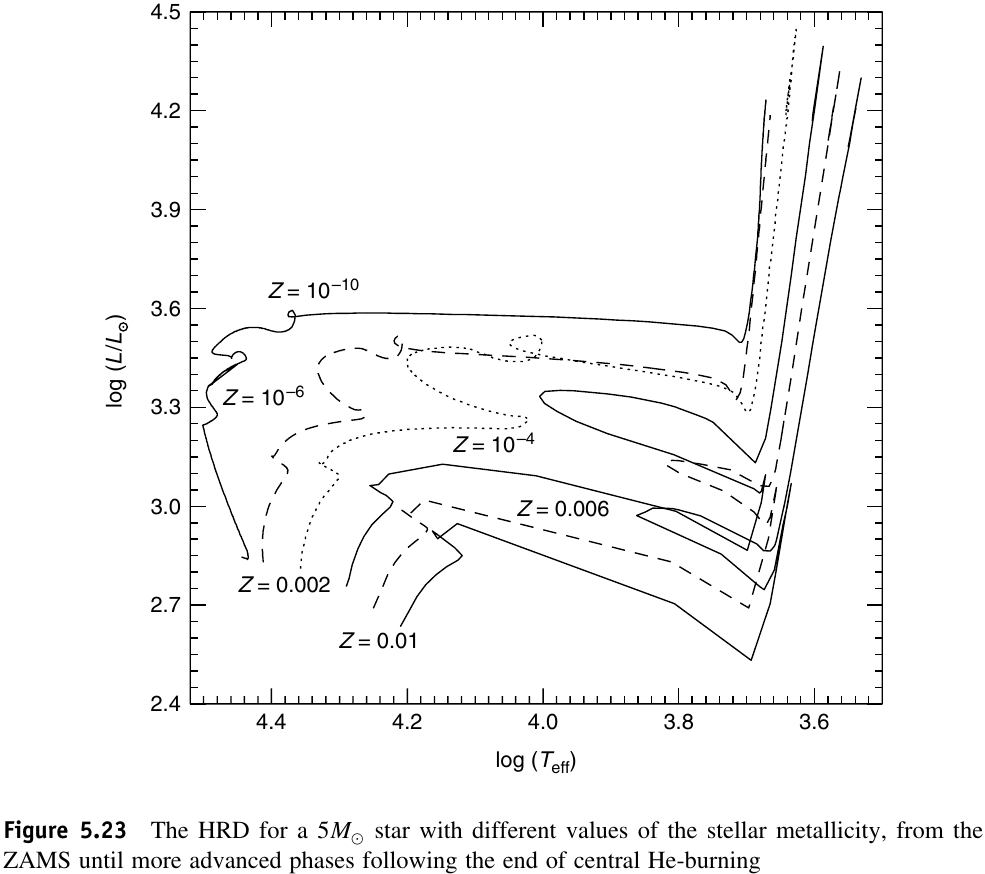
\includegraphics[trim={0cm 0cm 0cm 0cm},clip, keepaspectratio,width=0.85\textwidth]{lowZ5MsunHDR}\label{fig:lowZ5MsunHDR}
\end{figure}
    \end{column}
\end{columns}

\end{frame}

\subsection{Refs. HB}

\begin{frame}{Memo per HB}
combustion di He per stelle medio-grandi; clump He; loop He; Esaurimento He centrale: , semiconvezione e pulsi convettivi
\end{frame}

\subsection{He-burning reactions}

\begin{frame}{He-burning reactions}
\begin{columns}[T]\begin{column}{0.45\textwidth}
	\begin{align*}
&3\alpha (T\gtrsim\SI{1.2e8}{\kelvin}):\\ &^4He+^4He\to^8Be\tag*{$\tau_{1/2}\approx\SI{e-16}{\second}$}\\
&^8Be+^4He\to^{12}C+\gamma\tag*{$\SI{7.27}{\mega\ev}$, $\tau_H\approx100\tau_{He}$}\\
&\epsilon_{3\alpha}\approx\begin{array}{c}Y^3\rho^2T^{40}: T\approx\SI{e8}{\kelvin}\\T^{20}: T\approx\SI{2e8}{\kelvin}\end{array}
\end{align*}
Energy release per gram $Q/m(^{12}C)=\SI{5.9e17}{\erg\per\gram}$ - $1/10$ di quella prodotta da H-burning
	\end{column}
	\begin{column}{0.40\textwidth}
	\begin{align*}
&^{12}C+\alpha\to^{16}O+\gamma\tag*{Q=\SI{7.162}{\mega\ev}}\\
&^{16}O+\alpha\to^{20}Ne+\gamma\\
&^{20}Ne+\alpha\to^{24}Mg+\gamma\\
&^{24}Mg+\alpha\to^{28}Si+\gamma
\end{align*}
$\epsilon_{\alpha C}\propto YX_{12}\rho T^{20}$
\end{column}\end{columns}
\end{frame}

\subsection{Equilibrium model for low mass star after He-flashes: ZAHB}\linkdest{ZAHB}

\begin{frame}{Low Mass star HB: Flash-pulses to ZAHB and evolution from ZAHB}
    \begin{columns}[T]
        \begin{column}{0.55\textwidth}
\begin{figure}[!ht]
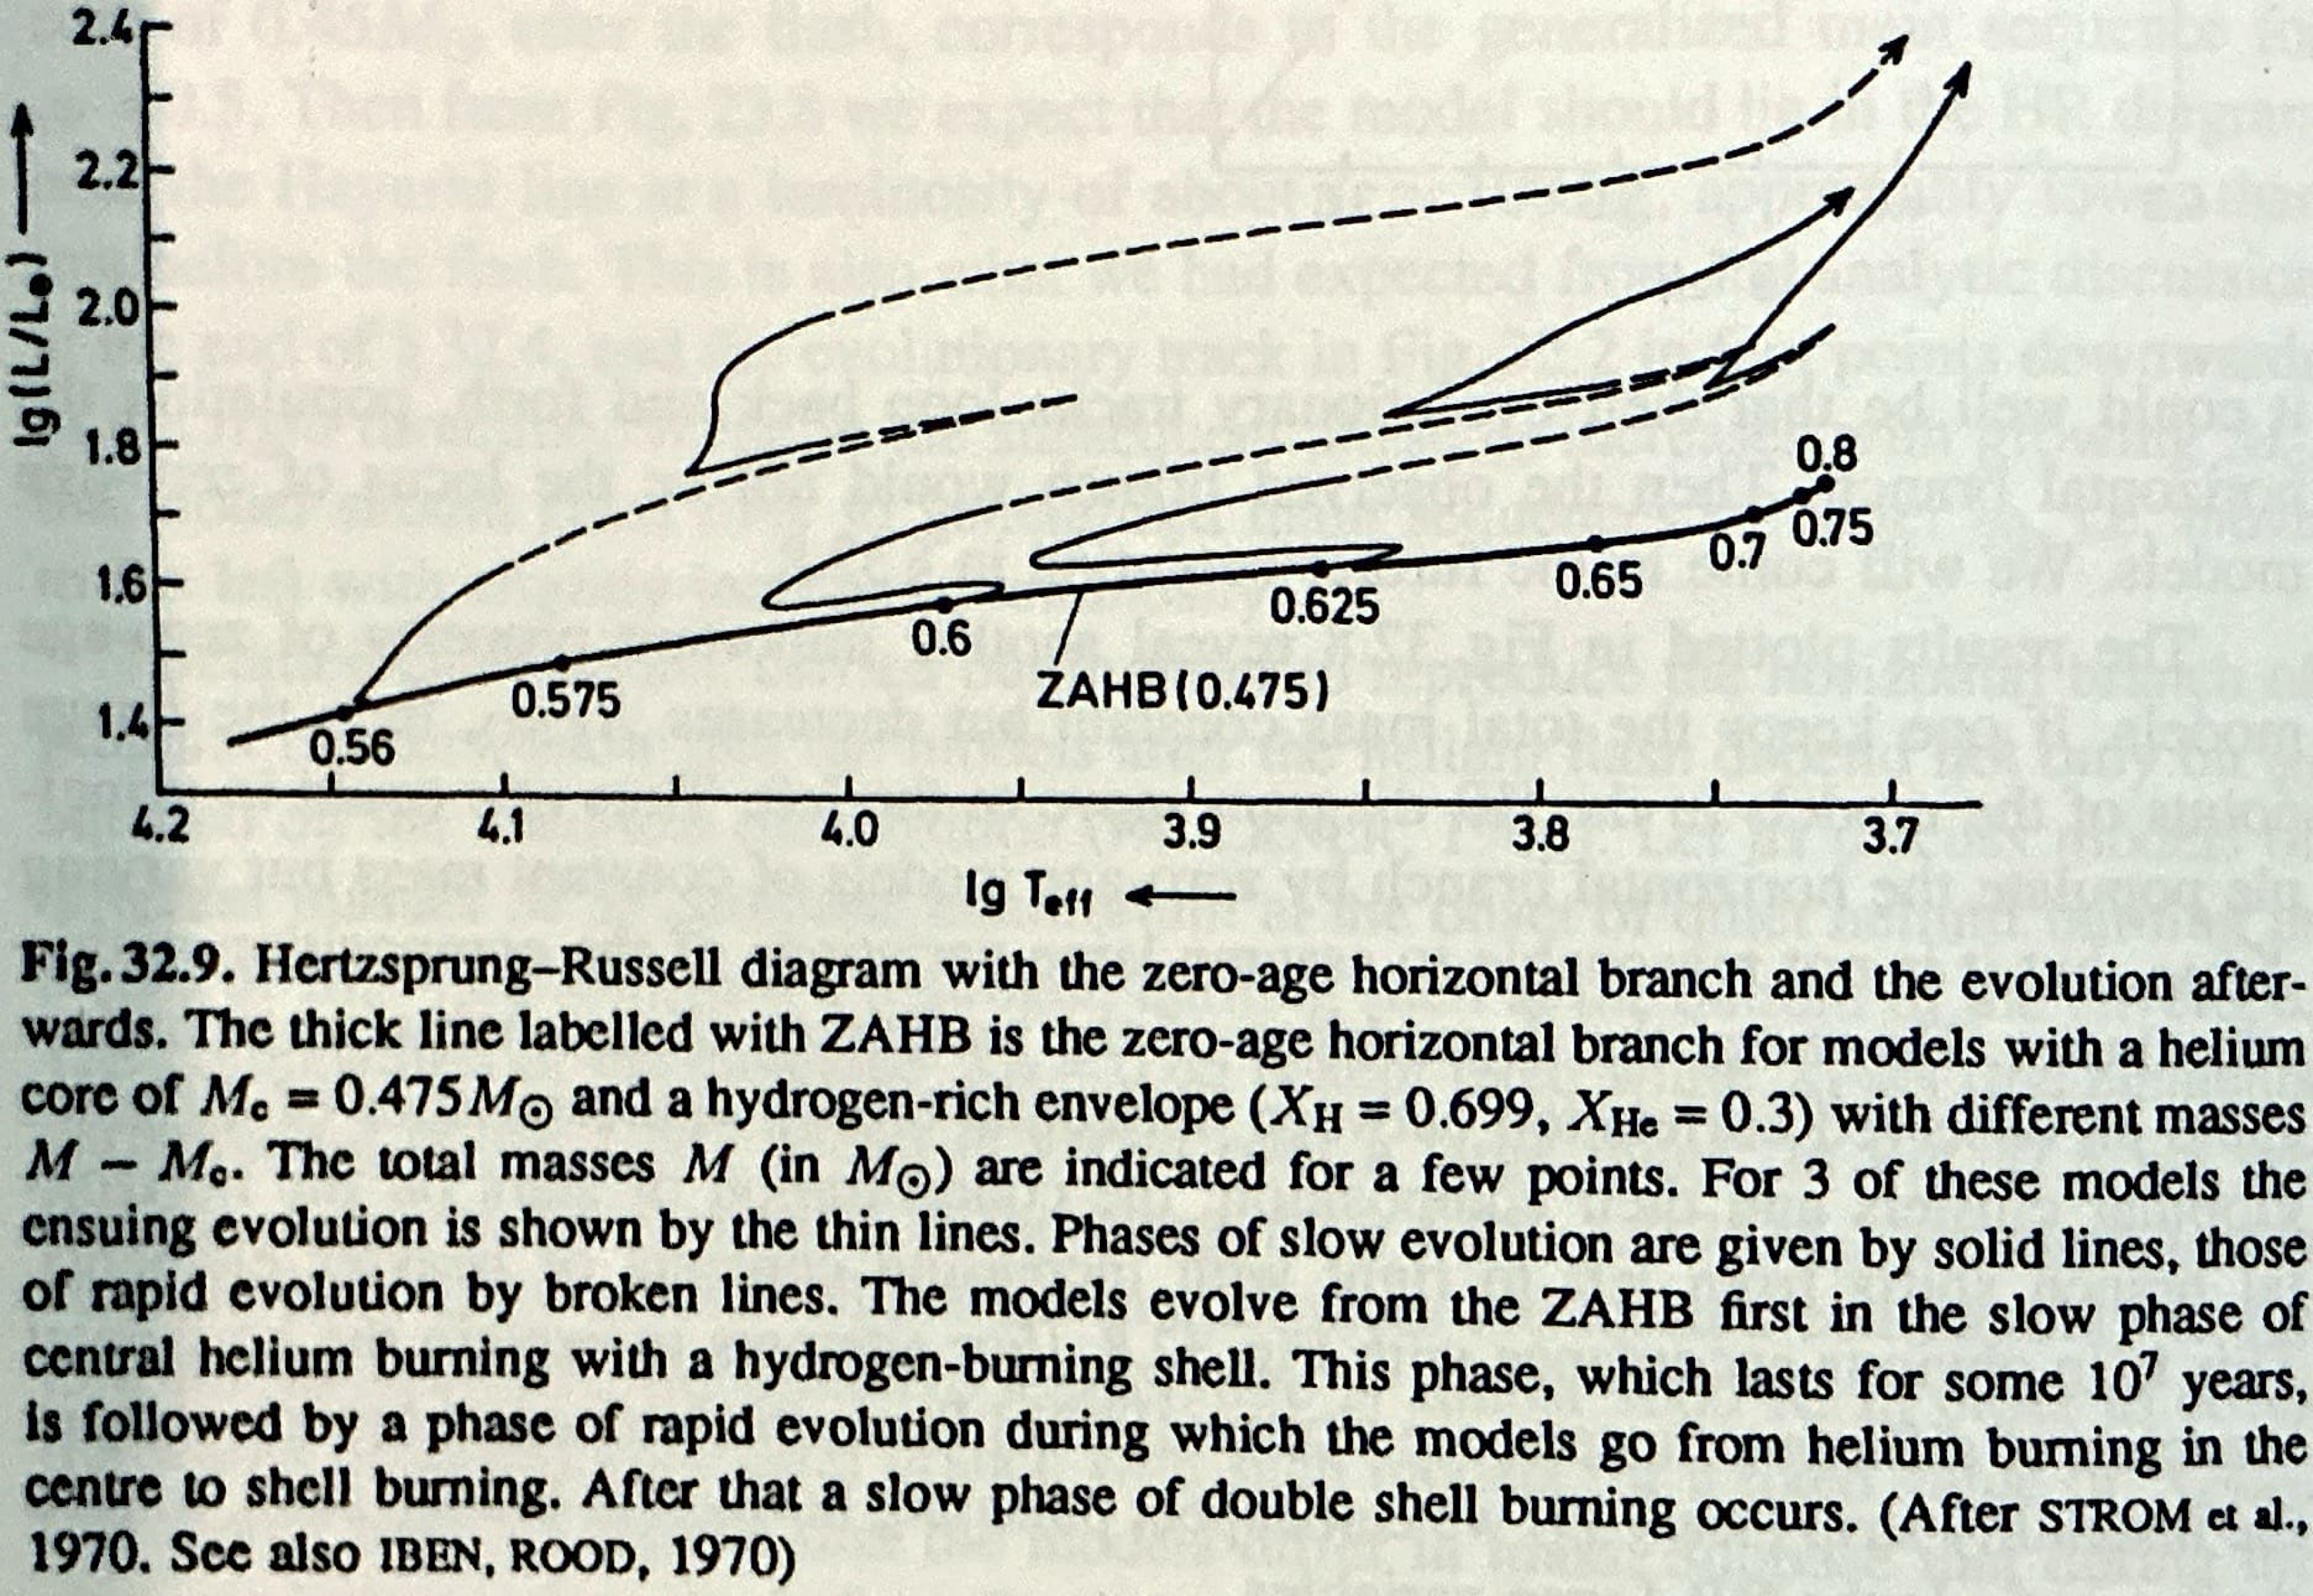
\includegraphics[trim={0cm 0cm 0cm 0cm},clip, keepaspectratio,width=0.75\textwidth]{evolfromZAHB}\label{fig:evolfromZAHB}
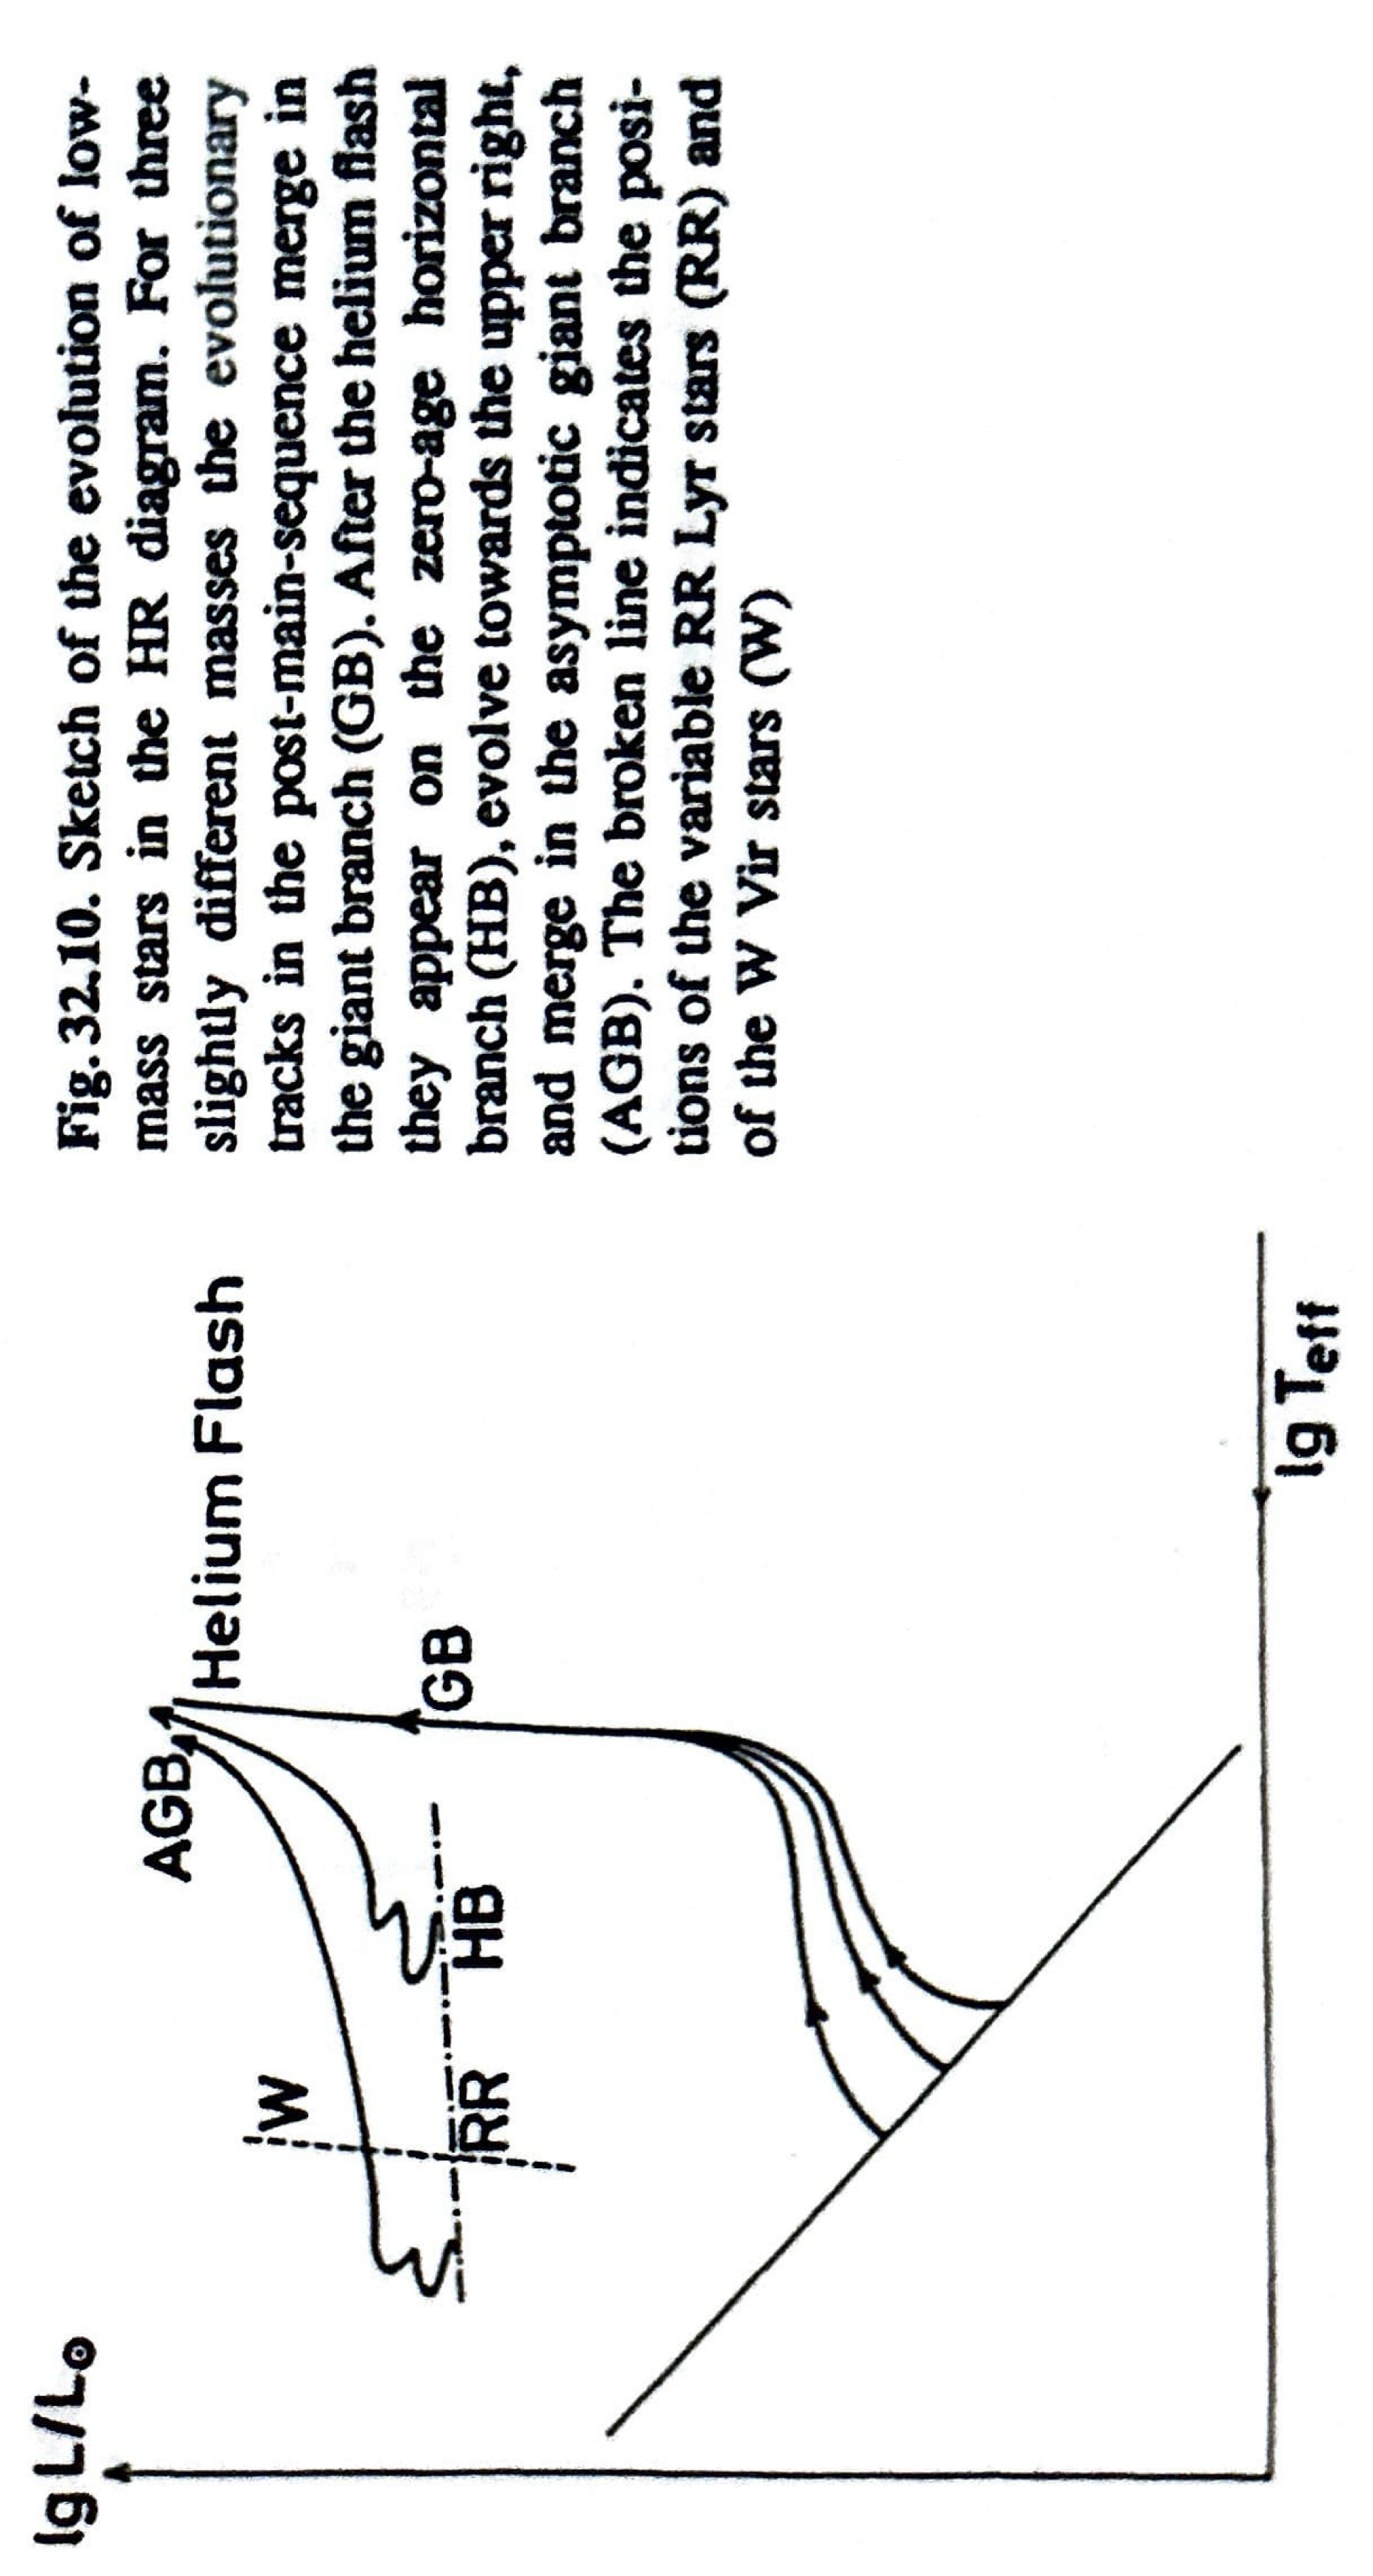
\includegraphics[trim={0cm 0cm 0cm 0cm},clip, keepaspectratio,height=0.75\textheight,origin=c,angle=-90]{Heflash2ZAHB}\label{fig:Heflash2ZAHB}
\end{figure}
        \end{column}
        \begin{column}{0.45\textwidth}
            \begin{itemize}
                \item He-pulses remove \Pelectron-deg from He-core: L drops 1 OM resp tip-RGB as core heating and expanding causes H-burning shell to cool down.
                \item Evolution from tip-RGB to He-burning very short: observing prob quite zero so many calculations begins from equilibrium model.
                \end{itemize}
        \end{column}
    \end{columns}
    
\end{frame}

\begin{frame}{ZAHB: equilibrium model} 
\begin{itemize}
    \item $\tau_{He-Flash}\approx\SI{e6}{\year}$: after that time of He-burning the \Pelectron degeneracy is removed (small obser. prob). Some authors start He-core evolution sequence from C enriched equilibrium model (C enrichment about $5\%$).
\item \keyword{ZAHB}: model where He is burnt into chem homo-core and H in shell with chem stratification He-flash like
\item He-enriched by I dredge-up: $\Delta Y\approx\numrange{0.02}{0.04}$.
\item Rotation (dalayed He-flash): \xaumenta{M_{cHe}}, \xdiminuisce{M_*} (mass loss), \xaumenta{T^{ZAHB}}/\xaumenta{L^{ZAHB}}
%\xaumenta{\epsilon_{He}}/\xdiminuisce{\epsilon_H}
\end{itemize}
\end{frame}

\begin{frame}{Another ZAHB ??}
\begin{columns}[T]
	\begin{column}{0.45\textwidth}
	\end{column}
	\begin{column}{0.45\textwidth}
		\begin{figure}[!ht]
			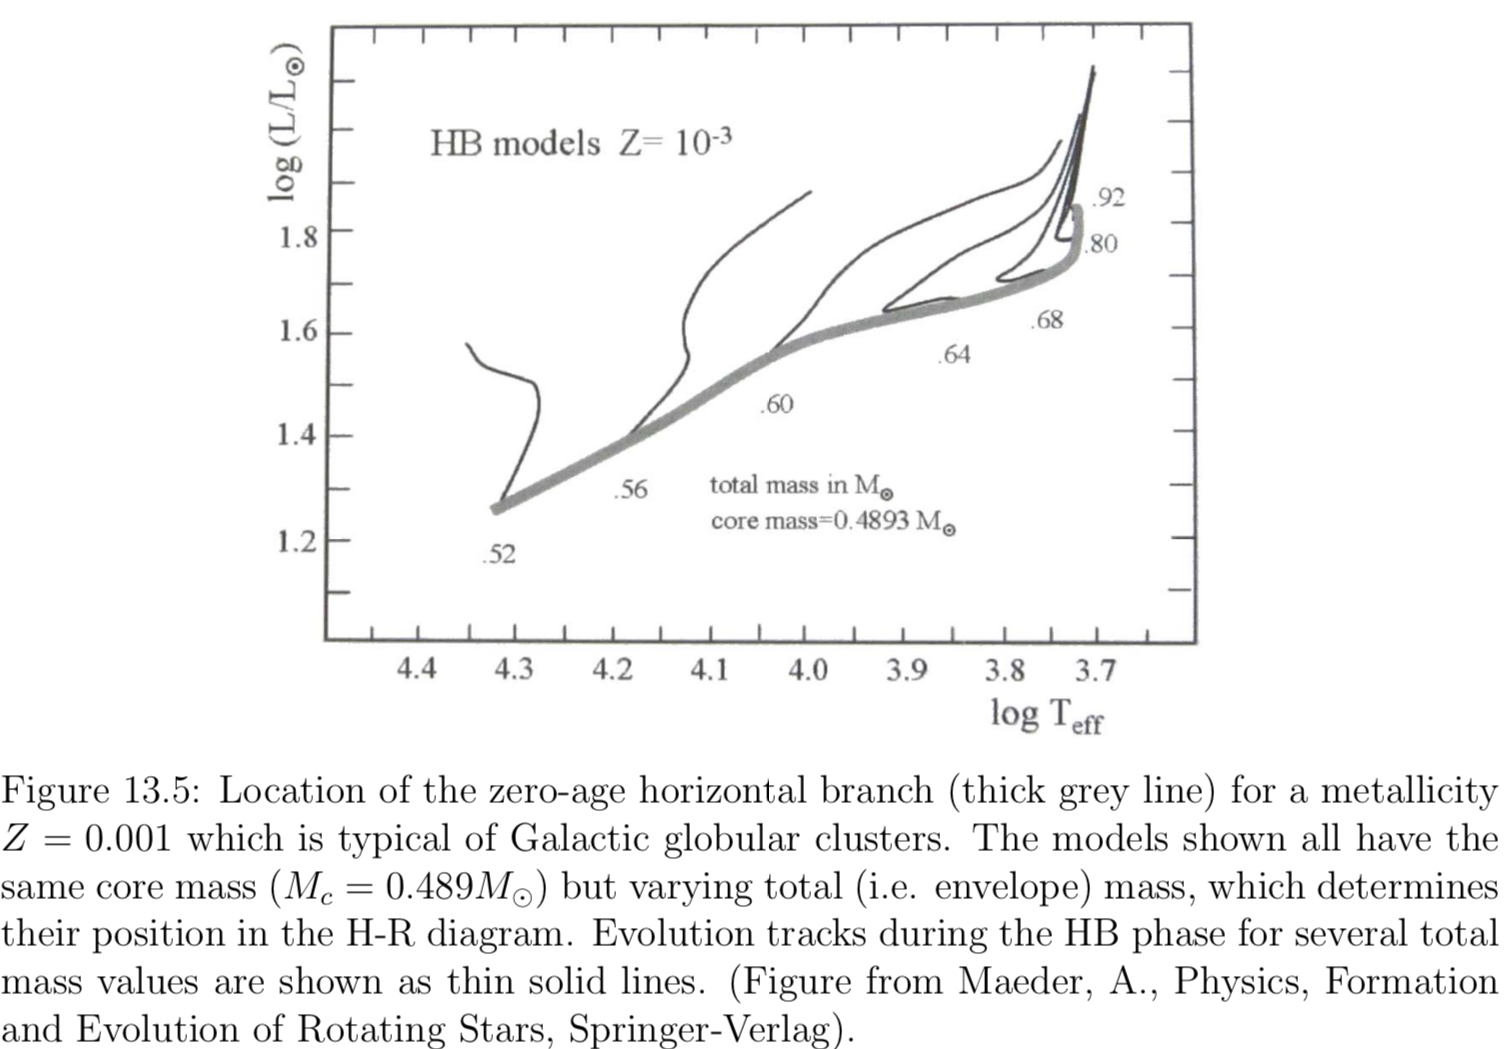
\includegraphics[trim={0cm 0cm 1cm 0cm},clip, keepaspectratio,height=0.37\textheight]{HB-ZA-evol}\label{fig:HB-ZA-evol}
		\end{figure}
	\end{column}
\end{columns}
\end{frame}

\begin{frame}{ZAHB dep on core (and  envelope) mass}
\begin{itemize}
\item Structure and evolution of ZAHB  fixed by: $M_*$, $M_{cHe}$ (for $M<1.8\msun{}$ $t_{TIP}>4-5\si{\giga\year}$: $M_c$ weakly dependent on M), $Y$, $Z_e$ - for low mass progenitors ZAHB is determined by Y, Z abundances of envelope and total mass - For fixed composition, $L_s$ is fixed by $M_{cHe}$ (then by $M_e$): important standard candles for Pop II stars (\keyword{Standard candles: HB brightness}). $(\TDy{M_{cHe}}{\log{L_{ZAHB}^{\log{T_e}=3.85}}})_{Y,Z}\approx3.04$
\item Location in HDR: \xdiminuisce{M_e }, \xaumenta{T_e} - HB (slightly oblique due to \xaumenta{\epsilon_H},\xaumenta{M_e}). $T_e\approx\SIrange{3500}{4000}{\kelvin}$ for $M_e\approx\numrange{e-4}{0.4}\msun{}$ (RGB mass loss)
\item \xaumenta{R_{cHe}}, \xdiminuisce{L_s} from RGB-tip as H-burning shell cool down
\item He-burning in convective core (steep T deps)
\item H-burning in shell: for fixed $M_{cHe}$ efficiency determined by \xaumenta{M_e}, \xaumenta{\epsilon_H}
\item HB-Brightness on of most important standard candles for PopII stars: L mainly fixed by $M_{cHe}$.
\end{itemize}
\end{frame}

\begin{frame}{ZAHB dep on composition}
\begin{columns}[T]
\begin{column}{0.55\textwidth}
\begin{itemize}
    \item \xaumenta{Y_{in}}, \xdiminuisce{M_{cHe}}, \xaumenta{L_H}/\xdiminuisce{L_{cHe}}, $L^{ZAHB}$ approx const: Blue (low mass envelope) part of ZAHB becomes fainter/ R part brighter. $(\TDy{Y}{L_{ZAHB}^{3.85}})_{M_{cHe},Z}\approx2.07$
\item \xaumenta{Z_{in}}, \xdiminuisce{M_{cHe}^{Flash}}/\xaumenta{\kappa_e}, \xdiminuisce{L^{ZAHB}}/\xdiminuisce{T_e^{ZAHB}}. $(\TDy{Z}{L_{ZAHB}^{3.85}})_{M_{cHe},Y}\approx-0.04$
\end{itemize}
\end{column}
\begin{column}{0.45\textwidth}
\begin{figure}[!ht]
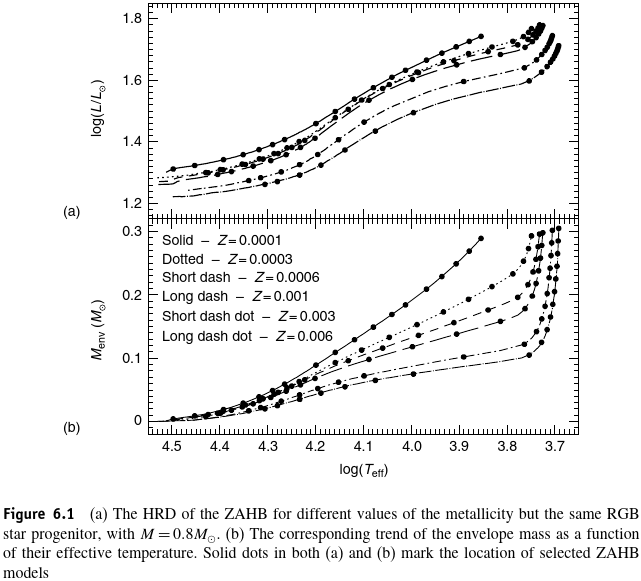
\includegraphics[trim={0cm 0cm 0cm 0cm},clip, keepaspectratio,height=0.37\textheight]{HDR-ZAHB-M08}\label{fig:HDR-ZAHB-M08}
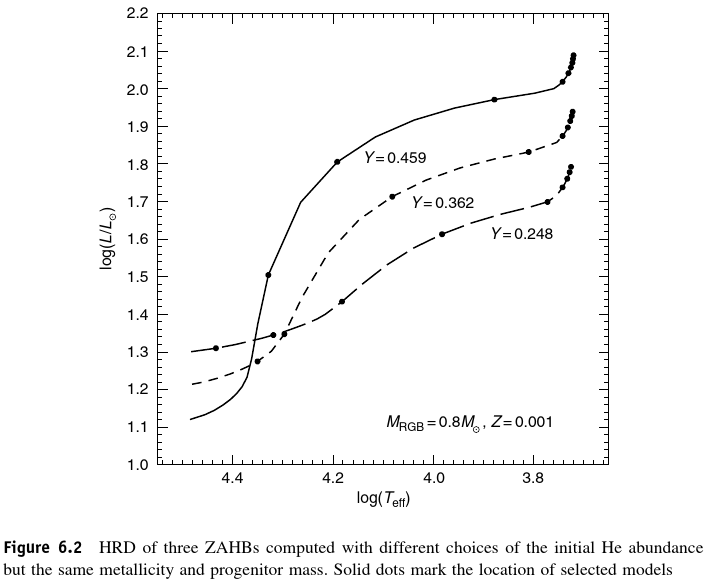
\includegraphics[trim={0cm 0cm 0cm 0cm},clip, keepaspectratio,height=0.37\textheight]{HDRZAHBdiffY}\label{fig:HDRZAHBdiffY}
\end{figure}
\end{column}
\end{columns}
\end{frame}

\subsection{Evolution from ZAHB: Core He-burning in low-mass stars}\linkdest{HBlowM}


%\TDy{}{}=\alpha\frac{dP}{P}-\delta\frac{dT}{T}+\phi\frac{d\mu}{\mu}
%dq=c_PdT-\frac{\delta}{\rho}\,dP
\begin{frame}{HB evolution in HDR}
\begin{columns}[T]
\begin{column}{0.4\textwidth}
\begin{itemize}
    \item \xaumenta{\epsilon_{He}}
    \item Loop: \xdiminuisce{\epsilon_H}: as $L_{He}<L_H$ star evolves at \xaumenta{T_e}, $L_{He}>L_H$ star moves toward R.
    \item Blue side (lower mass) go streight to Hayashi (\xaumenta{L},\xdiminuisce{T_e})??
\end{itemize}
\end{column}
\begin{column}{0.6\textwidth}
\begin{figure}[!ht]
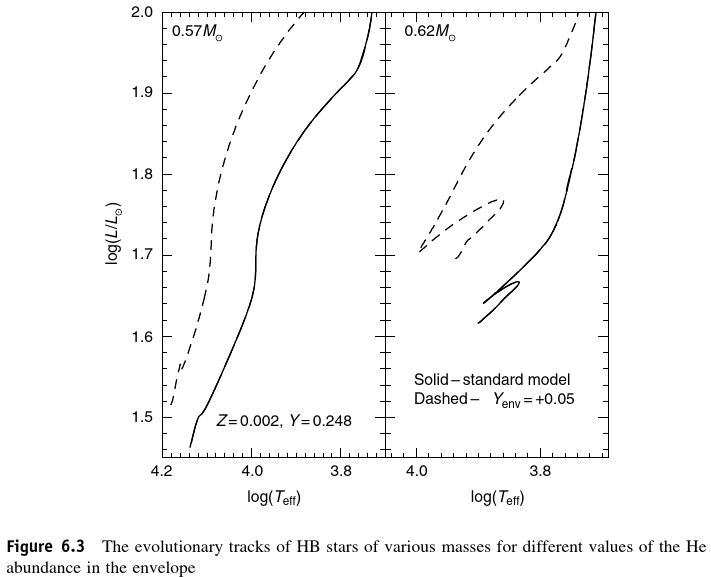
\includegraphics[trim={0cm 0cm 1cm 0cm},clip, keepaspectratio,height=0.6\textheight]{HB-lowM-evol}\label{fig:HB-lowM-evol}
\end{figure}
\end{column}
\end{columns}
\end{frame}

\begin{frame}{Mixinge Proc.: conv-inst at conv-boundary as \xaumenta{\kappa_{ff}},\xaumenta{\nrad} then semiconvection to $\nrad{}$ min}
\begin{columns}[T]
\begin{column}{0.5\textwidth}
    \begin{block}{Convective instability: extension of convective core follow increase $\nabla_{rad}$ - Autotrascinamento??}
Mixing processes in convective He-burning core: $\tau_{con}\ll\tau_{nuc}$, as $^4He\to^{12}C$, \xaumenta{\kappa_{ff}} ($\propto X_iZ_i^2$), \xaumenta{\nrad{}} - growing discontinuity in T gradient at convective core boundary - overshoot cause mixing with radiative shell: \xaumenta{\kappa} - convective instability of boundary - selfdriving mechanism for extension of convective core - Convective boundary is established where $\nabla_{ad}=\nabla_{rad}$
\end{block}
\begin{block}{semi-convection: decoupling of convective core and convective shell outside $\nabla_{rad}$ min}
    $\nrad{}$ show a minimum due to outward shift in He-rich environment due to self-driving mechanism (complex behaviour of $\nrad$ due to local L, T, $\kappa$, P).
    Region outside minimum of $\nrad{}$ cannot be mixed with core as at minimum $\nrad{}=\nad{}$, but the chemical composition is such that $\nad{}=\nrad{}$ in semiconvective shell.
    Effects: more extended loops on HRD; Core He-burning last longer; mass of He-depleted core at He-exhaustion is larger.
\end{block}
\end{column}
\begin{column}{0.5\textwidth}
\begin{figure}[!ht] 
%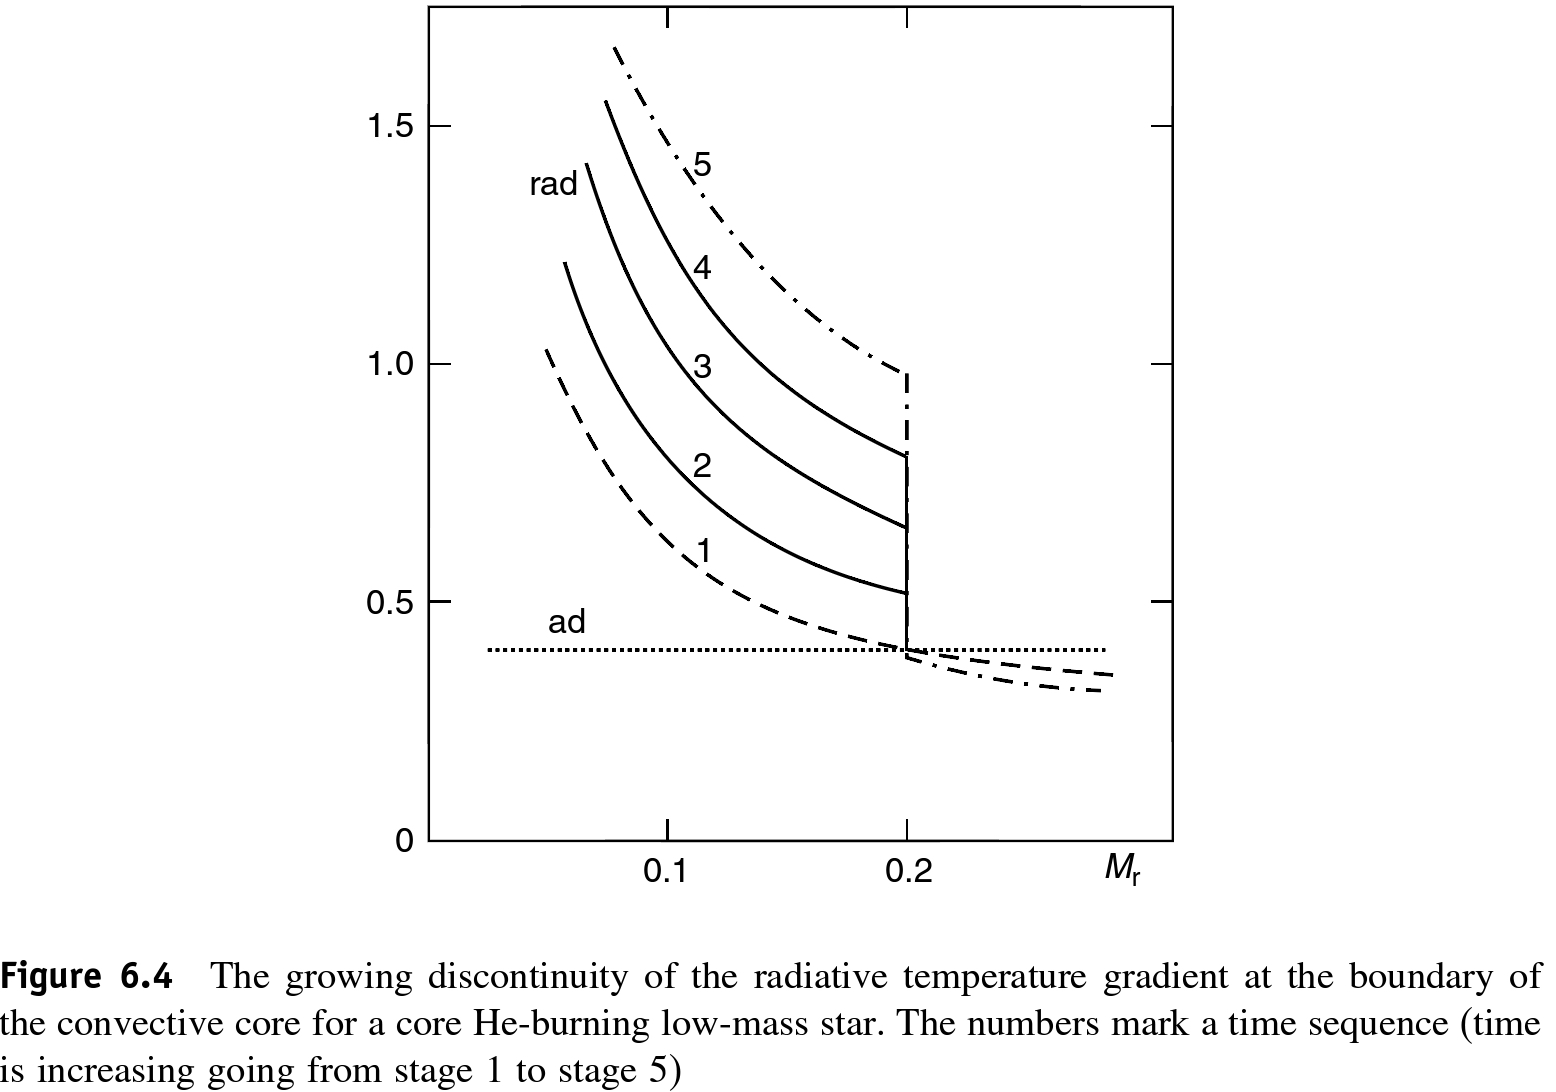
\includegraphics[trim={0cm 0cm 1cm 0cm},clip, keepaspectratio,height=0.4\textheight]{HBnrad-seq}\label{fig:HBnrad-seq}
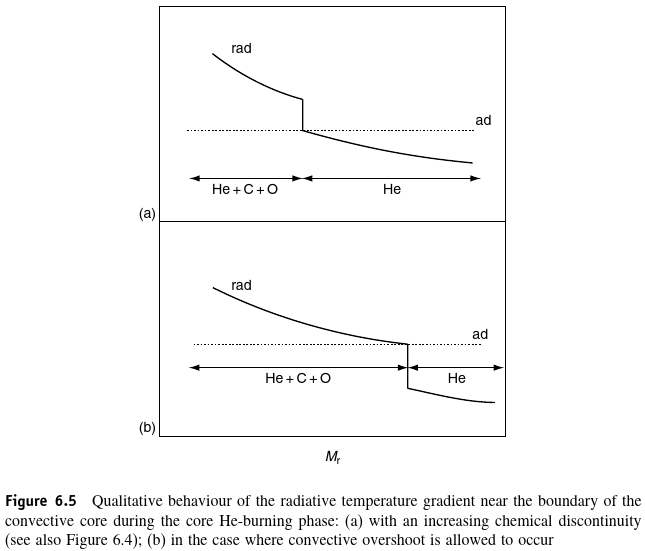
\includegraphics[trim={0cm 0cm 0cm 0cm},clip, keepaspectratio,height=0.45\textheight]{HBnablaraddisos}\label{fig:HBnablaraddisos}
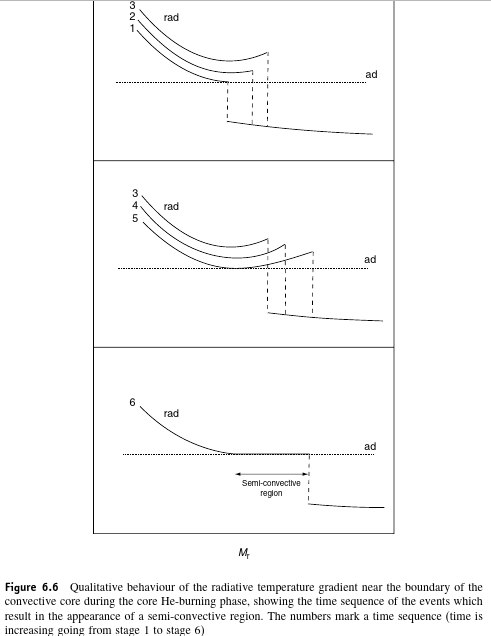
\includegraphics[trim={0cm 0cm 0cm 0cm},clip, keepaspectratio,height=0.45\textheight]{HBnablaraddiscsc}\label{fig:HBnablaraddiscsc}
\end{figure}
\end{column}
\end{columns}
\end{frame}

\begin{frame}{Breathing pulse (Pulsi convettivi) and obser vative consequences}
\begin{columns}[T]
	\begin{column}{0.4\textwidth}
	\begin{itemize}
        \item When $Y=0.1$ in cc $\alpha$-capture by $^{12}C$ tends to overcome $^{12}C$ production by $3\alpha$: $^{16}O$ has larger opacity and increases semiconvection region, \xaumenta{Y}, \xaumenta{\epsilon_{3\alpha}}, \xaumenta{L}, \xaumenta{\nabla_{rad}} - Breathing Pulse.
        \item After pulse star readjust to burn steadly He
        \item Core convective instability - 3 breathing pulses are needed to completely exhaust He in core.
	\item Effects of BP - i) Loop in HDR at each pulse ii) He burning time increased iii) $M_{cc}$ CO-core increased
	\end{itemize}
	\end{column}
	\begin{column}{0.50\textwidth}
	\begin{figure}[!ht]
	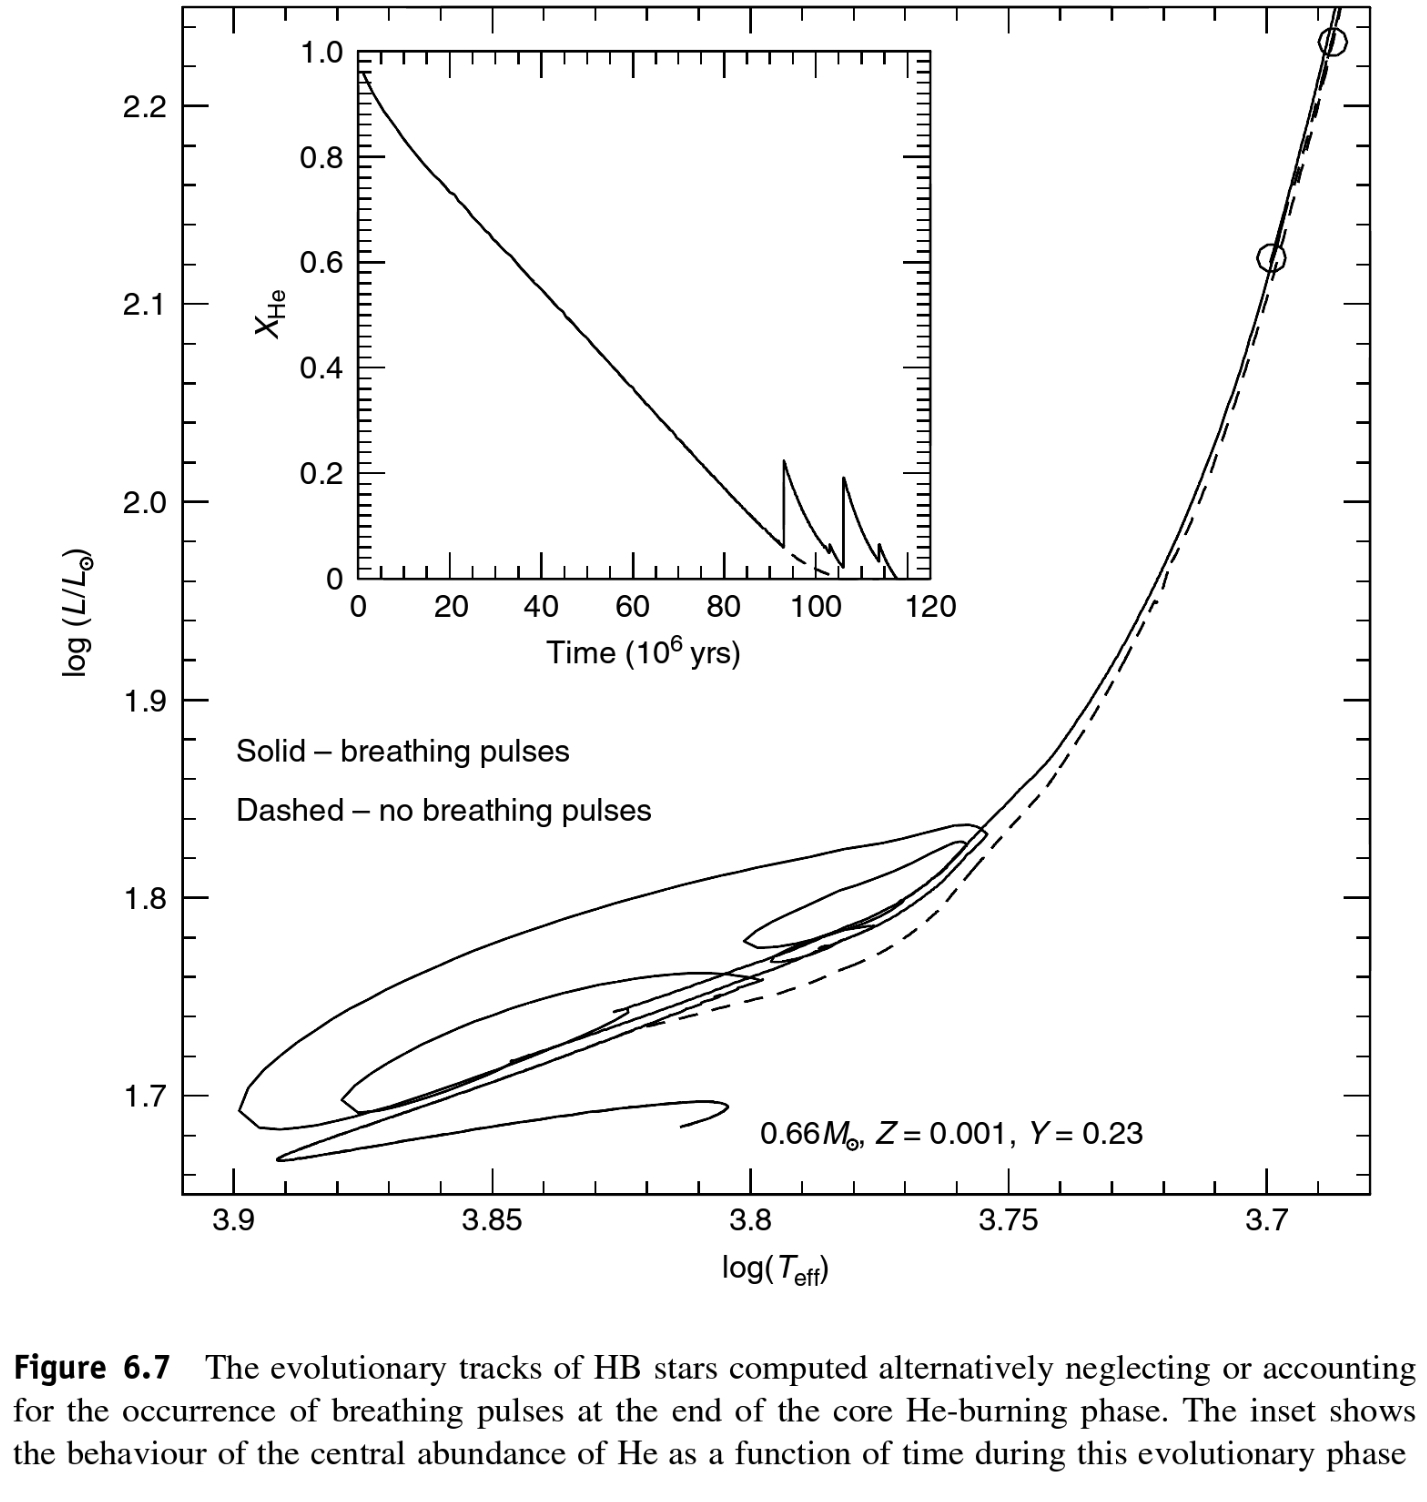
\includegraphics[trim={0cm 0cm 1cm 0cm},clip, keepaspectratio,width=0.95\textwidth]{HBbreathing}\label{fig:HBbreathing}
	\end{figure}
\end{column}\end{columns}
	\begin{itemize}
        \item R2 parameter - $R_2=\frac{t_{AGB}}{t_{HB}}\propto \frac{N_{AGB}}{N_{HB}}$: ratio of number of star in AGB to stars in HB (lifetime ratio) is sensitive to BP: $=0.12-0.15$ without BP, $0.8-0.14$ with BP - observed R2 in globular cluster ([36], [44]): BP efficiency very low, BP could be due to breakdown in instantaneous mixing approx in stellar models when convection setin in late HB stages
\end{itemize}
\end{frame}

\begin{frame}{Discussioni parametri che influenzano HB}
Parametro R per determinazione He
\end{frame}

\subsection{Core He-burning in Int/Mas stars}\linkdest{HBIM}

\begin{frame}{Evolution in HDR during HB for Int./massive star}
\begin{columns}[T]
	\begin{column}{0.55\textwidth}
	\begin{itemize}
        \item $M>2.3\msun$: He ignited at $T\approx\SI{e8}{\kelvin}$, $\rho_c\approx\SI{e4}{\gram\per\cubic\cm}$: No \Pelectron deg.(No He-flash) - He-burning phase: E to I.
        \item $\tau_{He}$ burning approx $20\%\tau_H$: \SI{22}{\mega\year} for $5\msun$, \SI{4}{\mega\year} for $10\msun$
	\item RGB climbing is reversed (fig: $E\to F$): star move toward B, energy released by H shell steadly increases until G where $L_{3\alpha}\approx20\%L$ then energy produced by H-burning shell decreases and models come back toward Hayashi track (\keyword{blue loop}) - long lasting phase so large observation prob in young galactic cluster.
    \item stars with $M>8-10\msun$ ignite He before RGB configuration: star move toward R and He burns in growing convective core, $L_s$ is mainly provided by H-burning shell.
	\item After He exhaustion we have condition for C ignition
	\end{itemize}
	\end{column}
	\begin{column}{0.45\textwidth}
	\begin{figure}[!ht]
	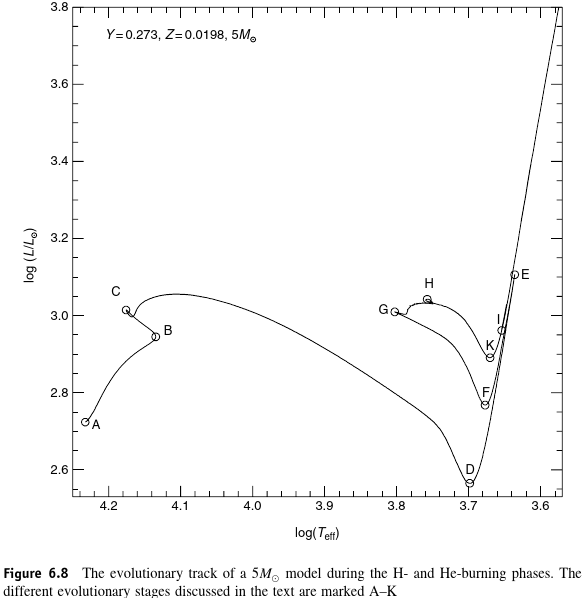
\includegraphics[trim={0cm 0cm 1cm 0cm},clip, keepaspectratio,height=0.4\textheight]{5MtoHB}\label{fig:5MtoHB}
	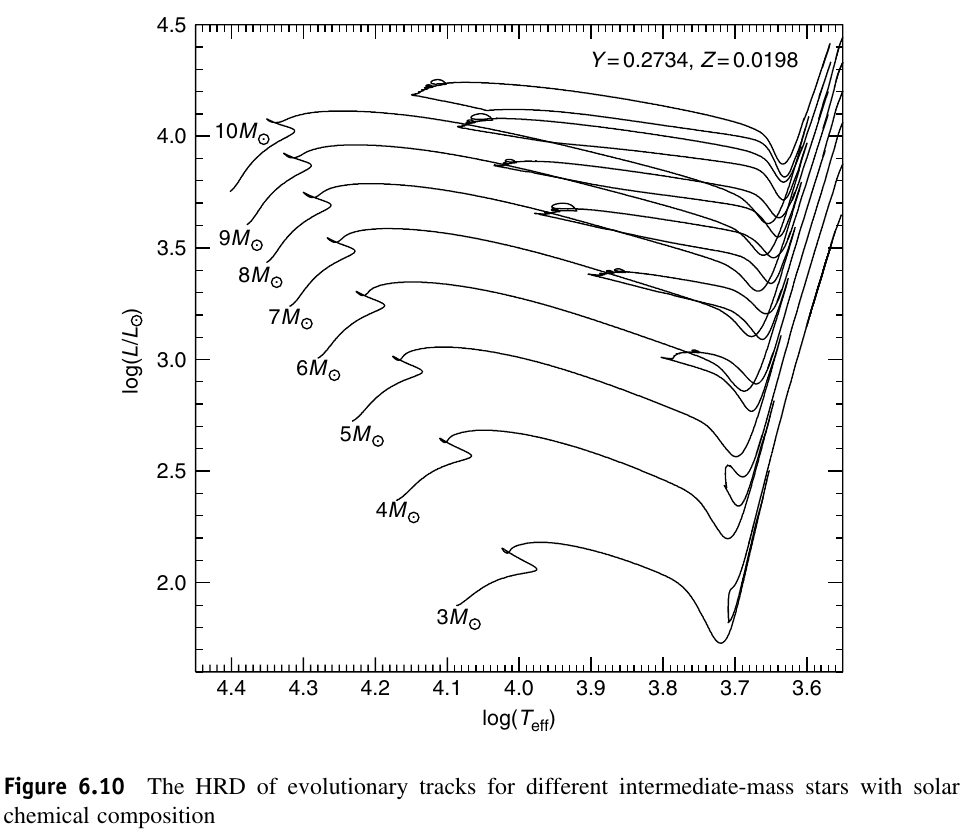
\includegraphics[trim={0cm 0cm 1cm 0cm},clip, keepaspectratio,height=0.4\textheight]{HRD-intermediate}\label{fig:HRD-intermediate}
	\end{figure}
\end{column}\end{columns}
\end{frame}

\begin{frame}{Deps of blue loop on params}
	\begin{itemize}
	\item Morphology of BL have non-linear dep on params [160]
	\item $M<10-12\msun$ B-loop increases with M, for more massive stars He ignites before Hayashi track - blue loop disappears
	\item extension B-loop increases, \xaumenta{Y}, decreases, \xdiminuisce{Z}
	\item B-loop seems favoured by sharper H profile in envelope (changes in H-burning efficiency as shell encounter discontinuity): CE overshoot produce enhanced discontinuity during dredge-up I: deeper convective envelope reaches regions more He-rich produced in MS
	\item increasing efficiency of overshoot of CC overshoot during H-burning strongly reduces B-loop extension
	\item If H-burning shell encounters chem. disc. before He-core ignition overshoot has no effect on B-loop
	\item Envelope overshoot may be able to trigger a B-loop: enhanced discontinuity during first dredge-up - deeper convective envelope reaches regions with more He produced in MS
	\item Increase of CC overshoot during H burning strongly reduces extension of B-loop
\end{itemize}
\end{frame}

\subsection{Pulsations of He-core burning stars - standard candles for PopI and PopII}\linkdest{HBpulsating}

\begin{frame}{instability strip: Cepheids and RR Lyrae}
%Refs: [61], [79], [80]
\begin{columns}[T]
	\begin{column}{0.65\textwidth}
	\begin{itemize}
	\item stable radial pulsation : $\kappa$-mechanism - star energy flow fixes the radius - stability implies variation in energy flux and thus in R - opacity increases during compression/decreases in expansionat same level in stellar envelope: He/H ionization ragions
    \item Boundary of IS - cool boundary: \xdiminuisce{T_e}, convection set in - hot boundary: \xaumenta{T_e}, \xdiminuisce{M_{ion}} (\xdiminuisce{\rho_{ion}}), \xaumenta{R_{ion}}
    \item Adiabatic pulsation with period $\Pi\sqrt{\rho}=Q$, slightly deps on M: $\Pi\propto \sqrt{\frac{R}{g}}\propto \frac{R^3}{M}$ as $g\propto \frac{M}{R^2}$. P-L relation: scale-distance of universe
\end{itemize}
\begin{block}{RR-Lyrae}
    \begin{itemize}
        \item RR-Lyrae: Low mass stars crossing IS during core He-burning. RR lyrae associated to globular cluster and found at all galactic latitude; RR lyrae are fainter than classical cepheids.
			\item He ionizati on region is $\num{e-7}\msun$, R varies by $20\%$, L by factor 2, $\Pi\approx0.2-0.9\si{\day}$ amplitude \SIrange{0.2}{1.6}{\mag} in B-band - ab-type fundamental tone (asymmetric), c-type (symmetric) first overtone,
            \item Blue edge of IS at $T_{eff}\approx\SI{7200}{\kelvin}$ at ZAHB luminosity level: for given mass and L, as $T_e$ increases there is less mass above ionization zone.
        \end{itemize}
\end{block}
\begin{block}{Classical Cepheids}
    \begin{itemize}
        \item $L\approx300-2500\lsun$, $\Pi\approx1-50\si{\day}$. Topology of cepheids IS is very diff from RR-Lyrae ([18]); \xaumenta{Z}, \xdiminuisce{T_e}: steeper IS. Int-mass stars going through He-burning with B-loop extends to IS.
        \end{itemize}
\end{block}
    \end{column}
	\begin{column}{0.35\textwidth}
	\begin{figure}[!ht] 
	%\includegraphics[trim={0cm 0cm 1cm 0cm},clip, keepaspectratio,height=0.37\textheight]{ffiig}\label{fig:ffiigg}
	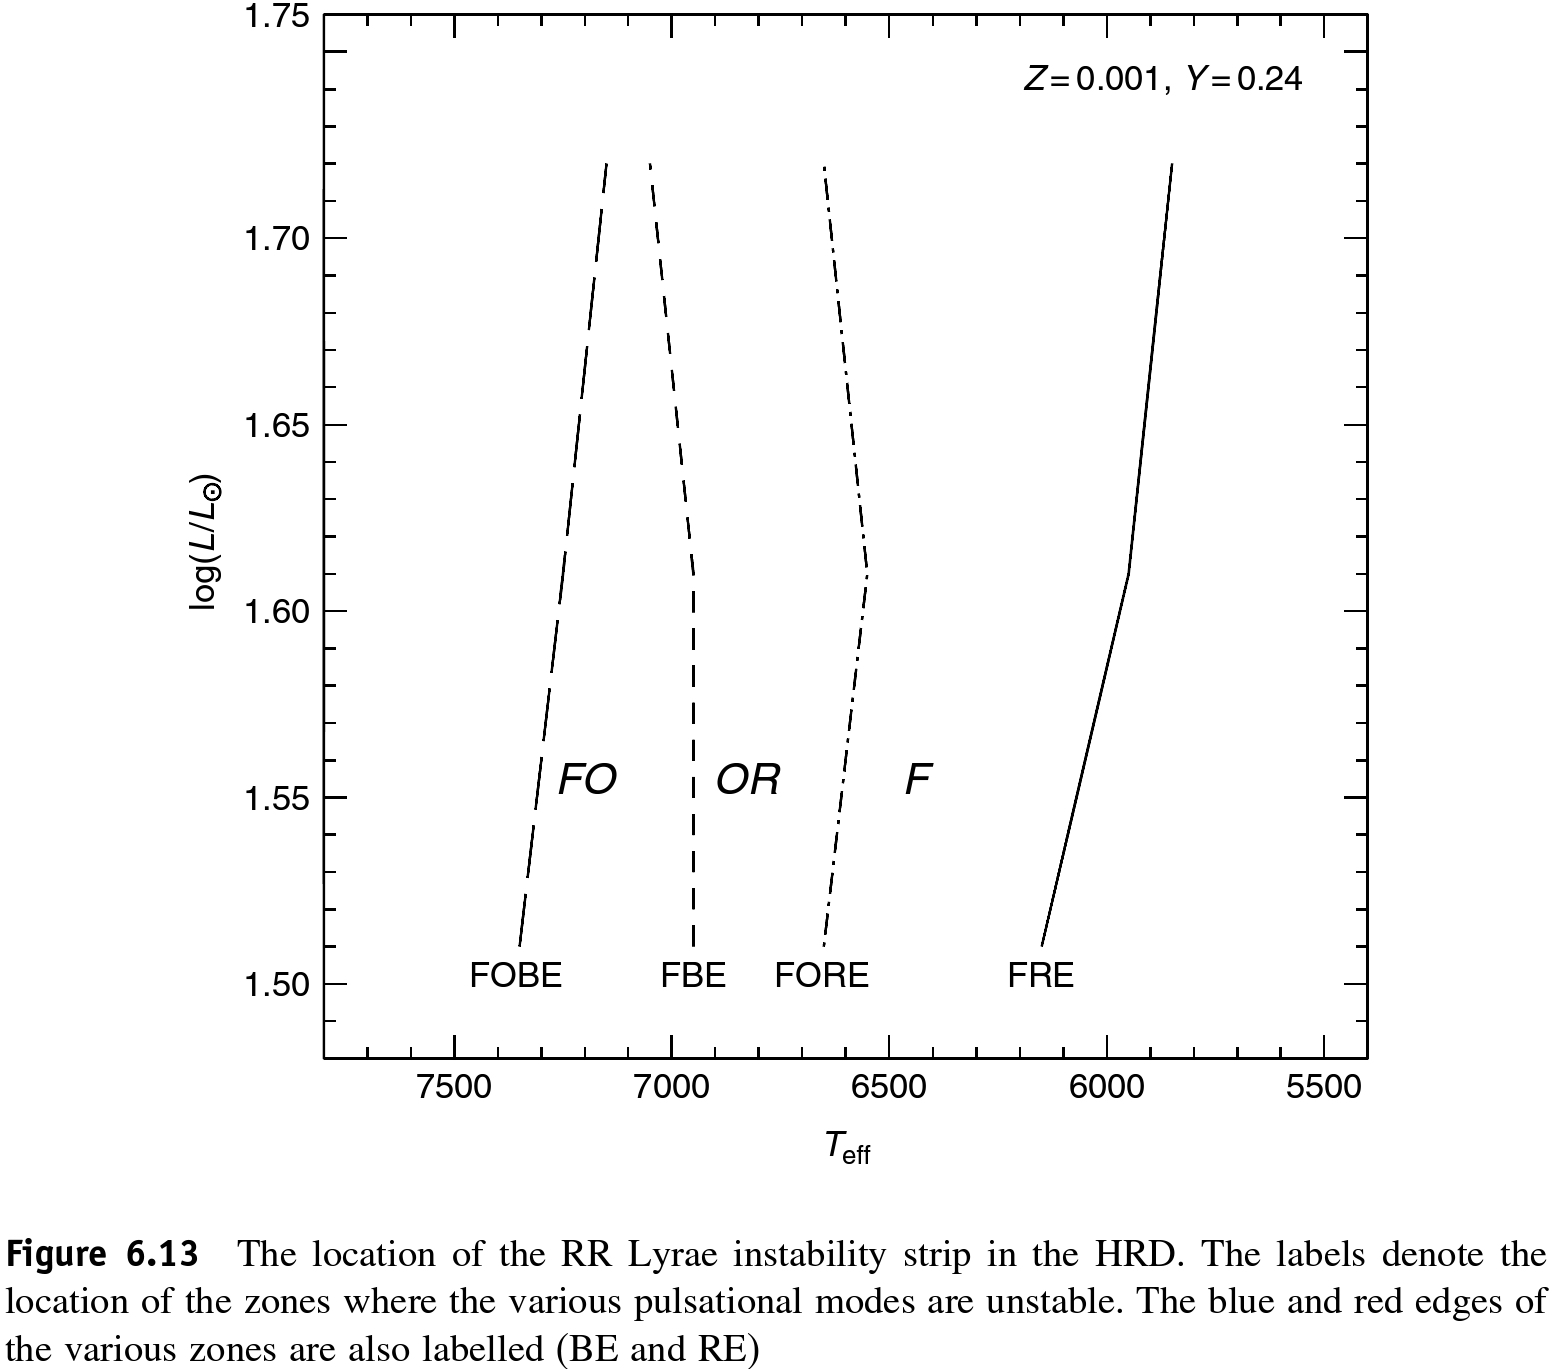
\includegraphics[trim={0cm 0cm 0cm 0cm},clip, keepaspectratio,height=0.43\textheight]{HBPulsation-RRIS}\label{fig:HBPulsation-RRIS}
	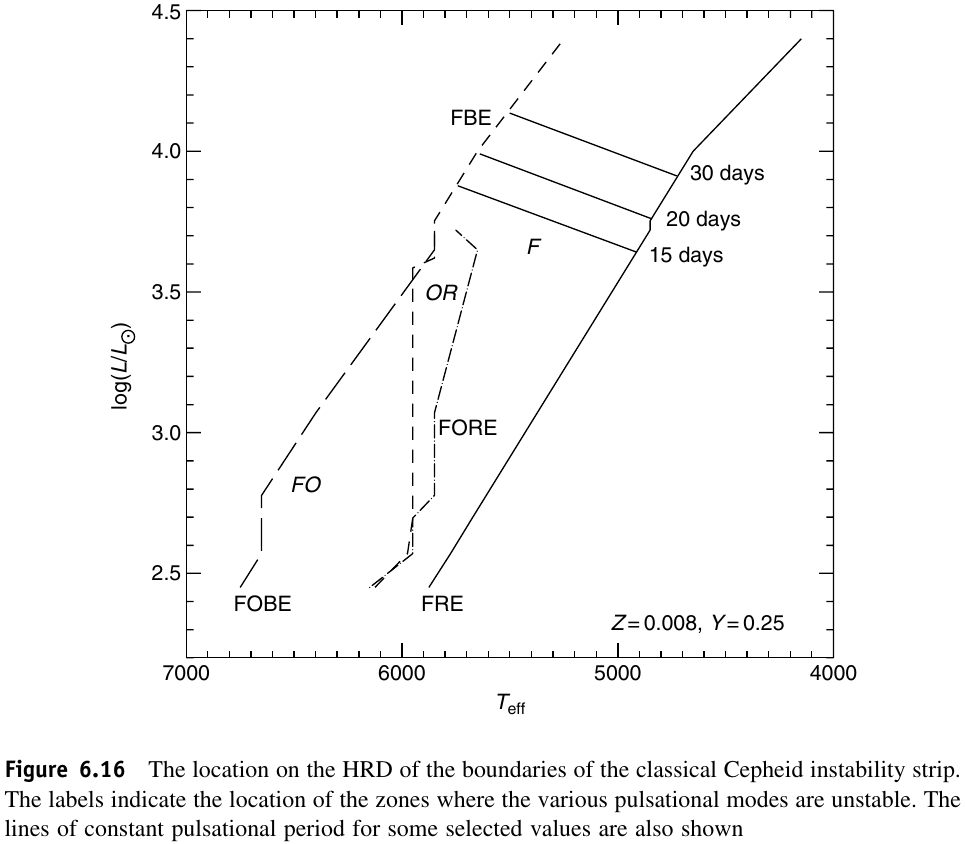
\includegraphics[trim={0cm 0cm 0cm 0cm},clip, keepaspectratio,height=0.43\textheight]{HBPulsation-CIS}\label{fig:HBPulsation-CIS}
	\end{figure}
\end{column}\end{columns}
\end{frame}

\begin{frame}{RR Lyrae and classical Cepheids: period-luminosity relation}
\begin{columns}[T]
	\begin{column}{0.7\textwidth}
        \begin{block}{RR-Lyrae}
        \begin{itemize}
            \item Moving to red: FO (first overtone stable), OR (both mode stable), F (only fundamental)
            \item Red edge at $T_e\approx\SI{5900}{\kelvin}$ envelope convection quenches pulsation.
	\item Petersen diagram: diagnostic tool for double-mode RR-Lyrae $\Pi_1/\Pi_0$ vs $\Pi_0$ - Bailey diagram: Comparison of theoretical/empirical result for amplitude vs $\Pi$
\item  Connection between $\Pi$ and other stellar parameter for ab-stars ([16]):
\begin{align*}
&\log{\Pi}=11.627+0.823\log(\frac{L}{\lsun})-0.582\log(\frac{M}{\msun})-3.506\log(T_e)\\
&=11.627+0.823A-3.506\log(T_e)\\
&A=\log{\frac{L}{\lsun{}}}-0.707\log{\frac{M}{\msun{}}}
\end{align*}
L of HB stars is strongly deps on Y ([35]): relation between $\Pi/A$ is usefull to infer $He_{in}$
        \end{itemize}     
        \end{block}
        \begin{block}{Classical Cepheids}
For solar composition and $\Pi_0$:
\begin{align*}
&\log{\Pi}=0.987-3.108\log{T_e}-0.767\log{\frac{M}{\msun}}+0.942\log{\frac{L}{\lsun}}\tag{theo}\\
&\exv{M_A}=a+b\log{\Pi}+c(CI)\tag{obs}
\end{align*}
The IS is shifted to red as Z increased ie toward longer period we should expect P-L relation deps on Z.
CI=color index. Tight relation between mass and surface luminosity of stars at beginning of He-core burning.
        \end{block}
    \end{column}
	\begin{column}{0.3\textwidth}
	\begin{figure}[!ht] 
	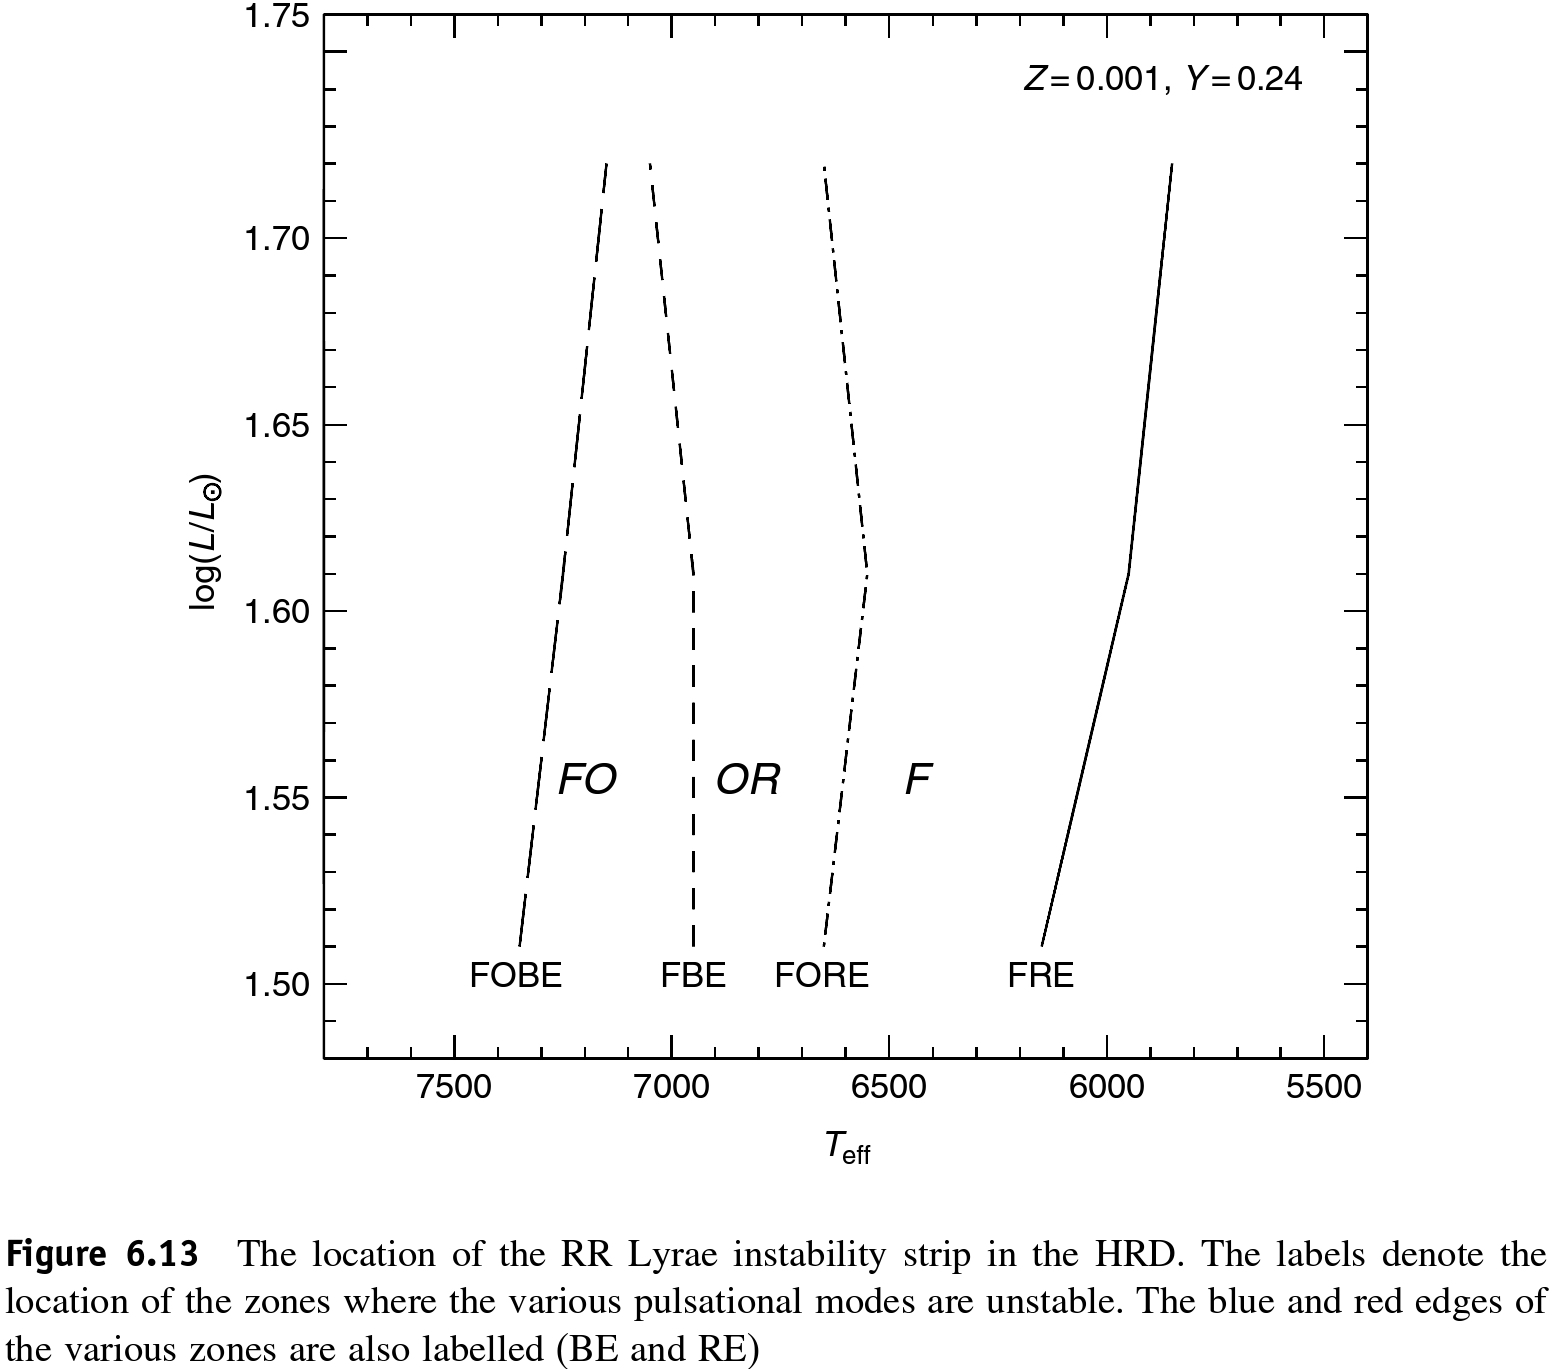
\includegraphics[trim={0cm 0cm 0cm 0cm},clip, keepaspectratio,height=0.30\textheight]{HBPulsation-RRIS}\label{fig:HBPulsation-RRIS}
	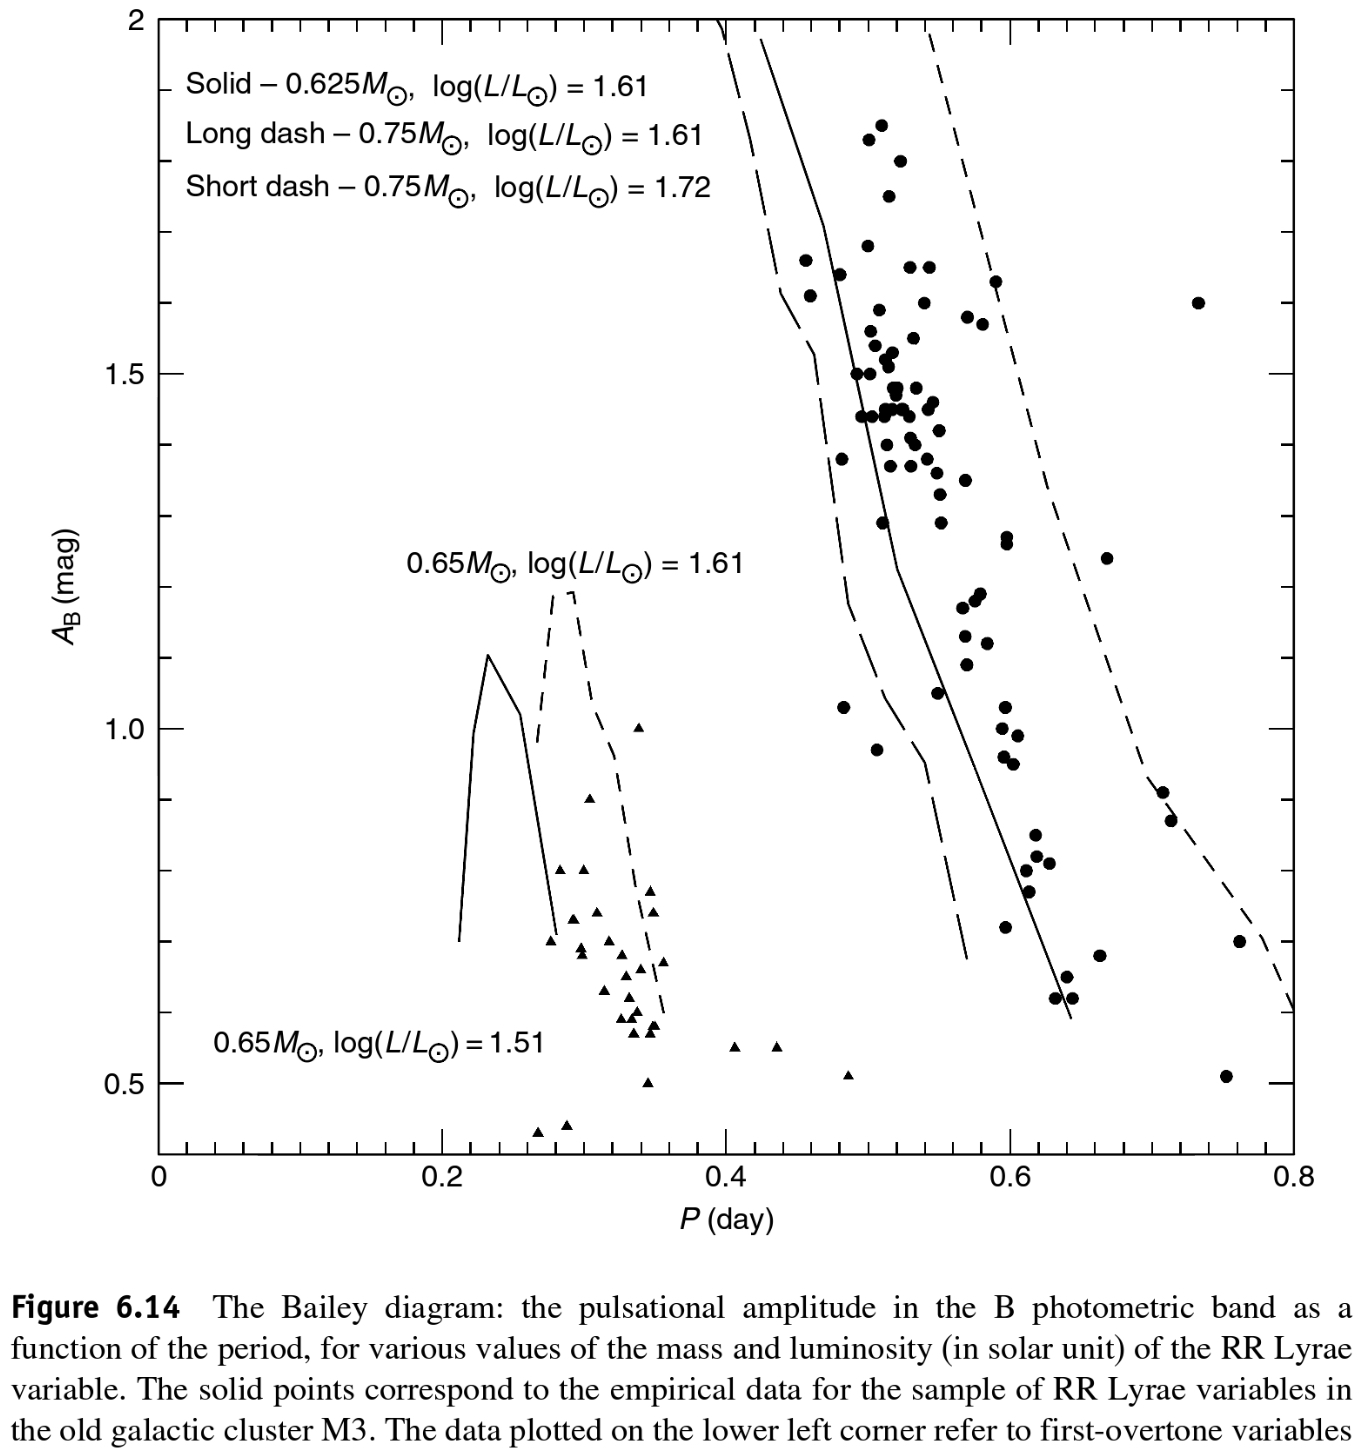
\includegraphics[trim={0cm 0cm 0cm 0cm},clip, keepaspectratio,height=0.30\textheight]{HBPulsating-B}\label{fig:HBPulsating-B}
	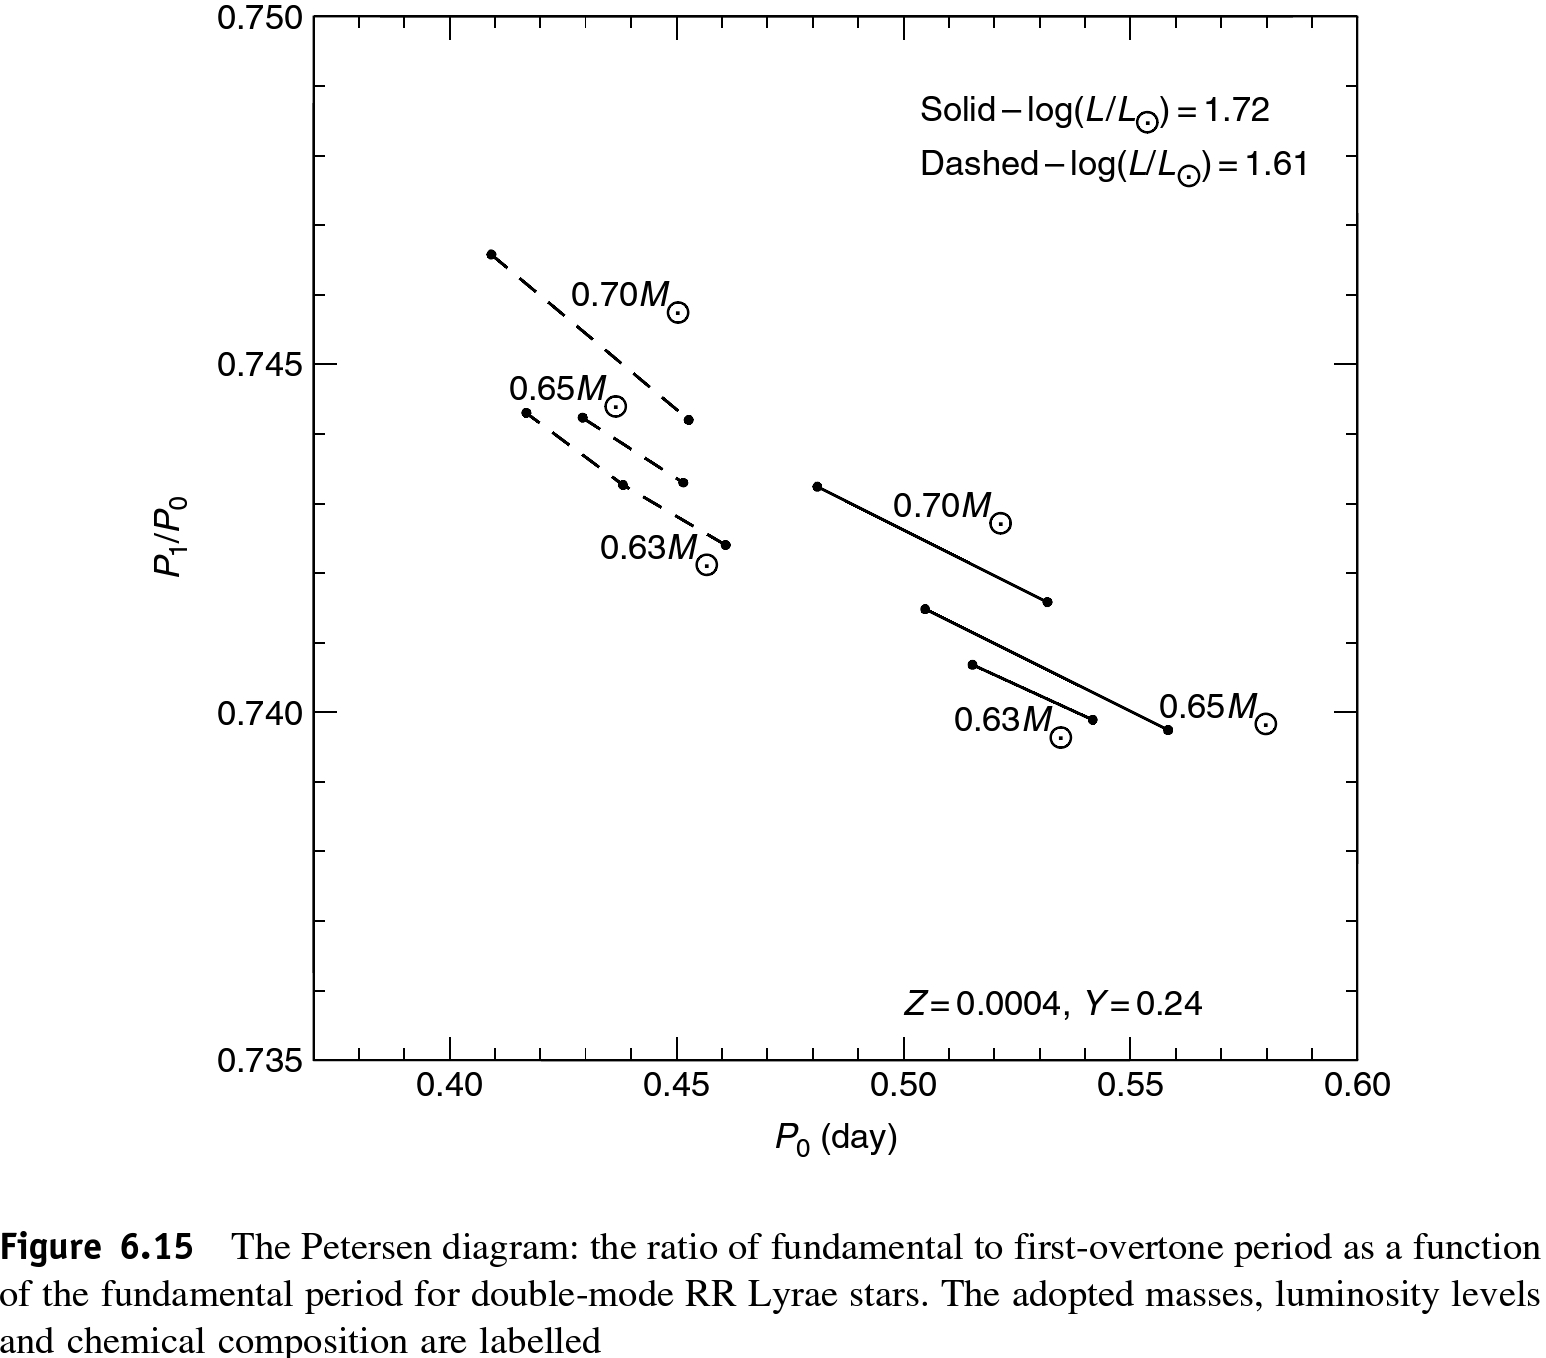
\includegraphics[trim={0cm 0cm 0cm 0cm},clip, keepaspectratio,height=0.30\textheight]{HBPulsating-P}\label{fig:HBPulsating-P}
	\end{figure}
\end{column}\end{columns}
\end{frame}

\subsection{Ramo asintotico (AGB)}\linkdest{AGB}

\begin{frame}{Index - Evoluzione in AGB}
Ingresso in agb: clump. AGB manqu\'e. Secondo Dredge-up; pulsi termici; terzo dredge-up
\end{frame}

\begin{frame}{Evoluzione in AGB: EAGB}
\begin{columns}[T]
	\begin{column}{0.45\textwidth}
	\begin{itemize}
	\item End of He-burning: He-core becomes low enough star move in HDR toward lower $T_e$/ larger $L$ (Asymptotic for $M_*<2.5\msun$): $T_e-L$ relationship similar to RGB (Hayashi track).
	\item Early AGB: He-burning shift to shell moving outward in He-core around CO-core of increasing mass due to $He\to C/O$ in shell; H-burning shell is turned off due to expansion caused by He-burning shell (T drops)
	\item \keyword{AGB clump}: in low $M_*$ onset of He-burning shell causes H-shell to switch off: \xdiminuisce{L_s} per ri-aumentare as \xaumenta{M_c} - stars cross 3-times same HDR region - well populated old galactic stellar system
	\end{itemize}
	\end{column}
	\begin{column}{0.50\textwidth}
	\begin{figure}[!ht]
	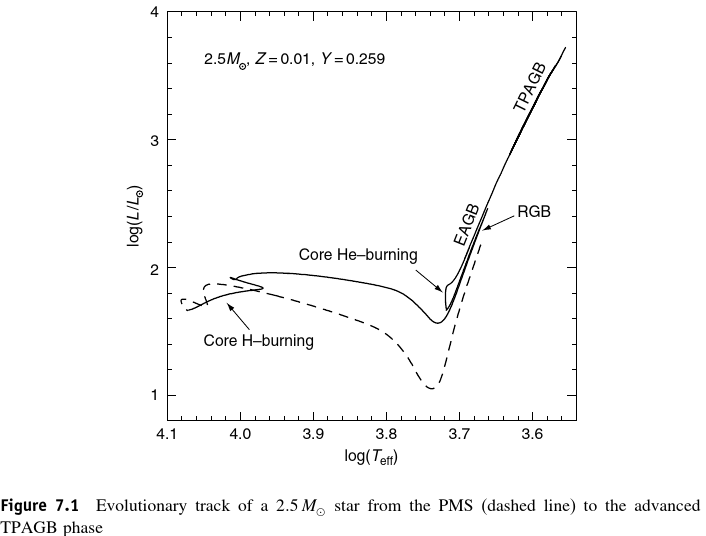
\includegraphics[trim={0cm 0cm 0cm 0cm},clip, keepaspectratio,height=0.4\textheight]{PMS2AGB-lowM}\label{fig:PMS2AGB-lowM}
	\end{figure}
    \keyword{Early AGB} and \keyword{second dredge-up}: for $M_*>3-5\msun$ (for lower mass H-burning shell remains efficient and prevent convection penetration) large flux by He-burning shell cause expansion of layers above and cooling let the outer convection penetrate H-depleted zone: up $1\msun$ of dredged-up material ($He$, $^{12}C,^{16}O\to^{14}N$); reduction of H-depleted region prevent formation of massive WD
\end{column}\end{columns}
Second dredge-up reduce mass of H-exhausted region preventing formation of massive WD (why?)
\end{frame}

\begin{frame}{CO-core state at end of HE-burning} 
\begin{itemize}
\item Plasma neutrino loss: $M_*<8-10\msun$ compact  CO-core with $\rho_C\approx\SIrange{e5}{e8}{\gram\per\cubic\cm}$ highly degenerate - plasma neutrino loss is balanced by contraction and cooling: cooling is max at center - $T_M$ moves outward
\item Limit mass $M_{up}$ where \Pelectron degener acy prevent CO-core ignition: depends strongly on initial composition - for solar composition $M_{up}\approx8\msun$, has minimum for $Z\approx0.001$ at $M_{up}\approx4\msun$
\item $M_*>M_{up}$: CO-core ignites (quitely/flash)
\item Stars igniting He core in non degenerat He core but develop degenerate CO core at nd of central He burning are intermediate-mass star; massive for $M>M_{up}$
\end{itemize}
\end{frame}
 
\begin{frame}{Thermally Pulsating AGB phase}
\begin{columns}[T]
	\begin{column}{0.45\textwidth}
 	When He-burning shell encounters H/He discontinuity dies - after rapid contraction H-burning shell provide star's energy needs - He ashes accreted on CO-core are compressed/heated until a critical mass is reached - $\approx\num{e-3}\msun$ for $0.8\msun$ CO-core - He ignited in runaway manner due to geometrical thickness of the shell - $L_{peak}\approx\numrange{e7}{e8}\lsun$.
	H-burning shell is turned of by expansion/cooling due to He-Burning - convective envelope from He-burning shell up to H/He discontinuity
	\end{column}
	\begin{column}{0.50\textwidth}
 		\begin{figure}[!ht]
			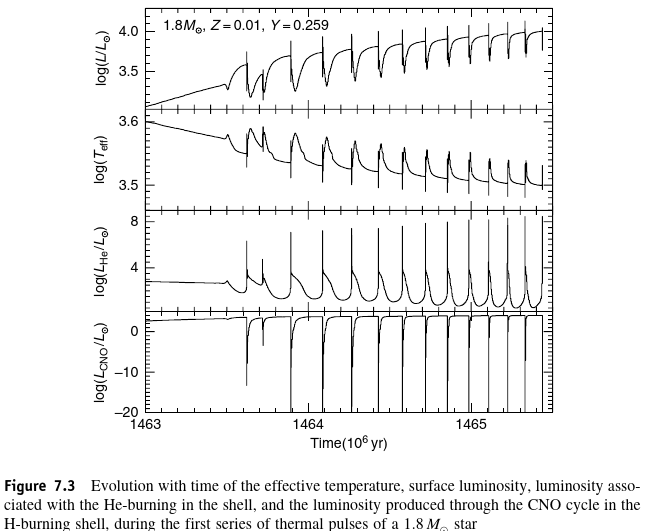
\includegraphics[trim={0cm 0cm 0cm 0cm},clip, keepaspectratio,height=0.45\textheight]{TPAGB-LTe}\label{fig:TPAGB-LTe}
		\end{figure}
        As \xdiminuisce{\epsilon_{He}} \xdiminuisce{L_{He}}: for $M_{CO}>0.7\msun$ decrese in L causes convective shell to disappear - for lower mass convection extends to incomplete He-burning regions: steady state nuclear burning and energy outflow.
\end{column}\end{columns}
After all product of H-shell is burnt H-burning shell turn on again (many repetition): pulse amplitude grows to asymptotic regime: $\epsilon_H$ depends on mass of He-core - $M_{cHe}-L_s$ relationship (as in RGB)
\end{frame}

\begin{frame}{\keyword{Properties of burning shell}}
Refs: [115], [155] - In a shell of thickness s located at r:
\begin{columns}[T]\begin{column}{0.5\textwidth}
\begin{align*}
&\frac{dP}{P}=4\frac{s}{r}\frac{d\rho}{\rho}\\
&(4\frac{s}{r}-\alpha)\frac{d\rho}{\rho}=\beta\frac{dT}{T}
\end{align*} 
\end{column}
\begin{column}{0.5\textwidth}
\begin{align*}
&\frac{dP}{P}=\alpha\frac{d\rho}{\rho}+\beta\frac{dT}{T}
\end{align*} 
\end{column}\end{columns}
Stable burning requires $4\frac{s}{r}>\alpha$ so if shell is too shallow an expansion causes \xdiminuisce{\rho} e \xaumenta{T}.
\end{frame}

\begin{frame}{Convective phenomena during TPAGB}
\begin{columns}[T]
\begin{column}{0.5\textwidth}
\begin{itemize}
\item After He-shell reignition convective envelope can move inward and cross H/He discontinuity: during \keyword{Dredge-up III} He-burning product/s-elements are dredged-up to surface (\keyword{C-star}: $O/C\ll1$ in photosphere) - \xaumenta{M_{DU}} as \xaumenta{M_C}, after maximum, \xdiminuisce{M_{DU}} as \xdiminuisce{M_e}
\item \xdiminuisce{Z}, DUIII penetrates deeper (difference surface abundance galactic AGB and Z poor AGB)
\item Convection penetrates deeper when pulse is stronger (more expansion/cooling): determined by thermal condition at bottom of He-rich layers - \xdiminuisce{\epsilon_H} maggiore \'e la densit\'a sul fondo di He-shell stronger TP - $\epsilon_H$ deps on $M_e$ (wind, burnt), H-exhausted region mass, chem-comp
\item Minimum for DUIII $M_e\approx0.4\msun$: $M_{ZAMS}<1.4-1.5\msun$ don't have DUIII - we don't expect C-rich stars in old pop
\end{itemize}
\end{column}
\begin{column}{0.5\textwidth}
\begin{figure}[!ht]
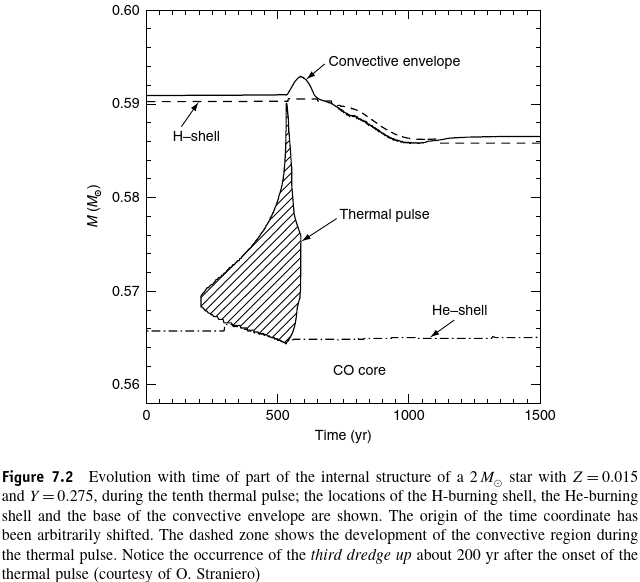
\includegraphics[trim={0cm 0cm 0cm 0cm},clip, keepaspectratio,height=0.45\textheight]{TPAGB-3DU}\label{fig:TPAGB-3DU}
\includegraphics[trim={0cm 0cm 0cm 0cm},clip, keepaspectratio,height=0.45\textheight]{C13-N14pocket}\label{fig:C13-N14pocket}
\end{figure}
\end{column}\end{columns}
\end{frame}

\begin{frame}{Nucleosintesi in AGB: s-elements}
\begin{columns}[T]
\begin{column}{0.45\textwidth}
\begin{itemize}
\item Spectr oscopical obs: AGB surface enriched of \keyword{s-elements} (Sr, Y, Zr, Ba, La, Ce, Pr, Nd) produced via ''slow'' neutron capture - $^{99}Tc$ on surface $\tau\approx\SI{2e5}{\year}$ prove it's not pollution due to accretion of primeval material
\item During first inter-shell mixing $^{14}N\to^{22}Ne$: $^{14}N(\alpha,\gamma)^{18}F(\beta+,\nu)^{18}O(\alpha,\gamma)^{22}Ne$.
\item if at T P at base of intershell $T>\SI{3.5e8}{\kelvin}$ first neutron production reaction take place as in int-M AGB ([103]), for $M_*<3\msun$ $T>\SI{9e7}{\kelvin}$ for second reaction
\end{itemize}
\end{column}
\begin{column}{0.5\textwidth}
    n production ([30,32]): Fowler Mechanism
\begin{align*} 
&^{22}Ne(\alpha,n)^{25}Mg\\
&^{13}C(\alpha,n)^{16}O
\end{align*}
[208]: 2nd fully burn C in rad region between 2 Pulses: \SI{e7}{\per\cubic\cm} neutron density. Rimozione di N (which capture n) da inter-shell:
\begin{align*} 
&^{14}N(\alpha,\gamma)^{18}F(\beta^+,\nu)^{18}O(\alpha,\gamma)^{22}Ne
\end{align*}
Produzione/distruzione di $^{13}C$
\begin{align*}
&^{12}C(H,\gamma)^{13}N(\beta^+,\nu)^{13}C\\
&^{13}C(H,\gamma)^{14}N
\end{align*}
\end{column}\end{columns}
\keyword{Tasca di $^{13}C$}: In inter-shell after convective episode is present $^{12}C$ but not $^{14}N$ - $^{13}C$ can be produced if right amount of H (diffusion, overshoot, rotational mixing, gravity waves) - [104]: after DUIII (\keyword{post-flash dip}) sharp disc. between H-rich env/He-/C-rich intershell until H-reignition (\SI{e4}{\year}) and then heated up form $^{13}C$
\end{frame} 

\begin{frame}{Hot-bottom burning ([209])}
$M_*>6-7\msun$ at base of convective zone ($T\approx\SI{8e7}{\kelvin}$) happens significant burn: \xaumenta{L_s} (breaks of $M_c-L$ relation) - s composition is strongly affected: $C\to N$, Li production through \keyword{Cameron-Fowler mechanism} [33] - when envelope has $T\approx\SI{e8}{\kelvin}$ $^3He+^4He\to^7Be+\gamma$ very efficiently then $^7Be+\Pelectron\to^7Li+\Pnue$: $^7Li$ can survive $T<\SI{2.5e6}{\kelvin}$. Amount of surface-Li after envelope retreats is determined by balance of $^7Be$ transported toward surface and Li produced at $T<T_b$ transported inside. [231]: Brightest long period variables (TPAGP experiencing large amplitude pulsation) are super-Li object (3 O.M. then expected)
\end{frame}

\begin{frame}{AGB termination}
\begin{columns}[T]
	\begin{column}{0.40\textwidth}
	\begin{itemize}
	\item $M_*>1.4\msun$ (Chandrasekhar limit): C-ignition, AGB ends - we don't expect $M_{CO}$ becomes suff. larger during TPAGB (mass loss)
	\item When $M_e<\num{e-3}\msun$, $\epsilon_H\to0$, \xaumenta{T_e} - \keyword{superwind} terminate AGB phase - brightest AGB in different systems show same luminosity: mass loss strongly increases at AGB's end ($\num{e-4}\msun\si{\per\year}$)
	\item Evolution of low mass star: TPAGB to WD - once $M_e$ below critical limit star move \xaumenta{T_e} at constant L - burning H in thin shell until bluest point then both H-/He-rich envelope contracts rapidly. Thermal envelope conditions determine which: i) nuclear burning dies (WD) ii) Heating He-shell born-again AGB (runaway He-burning then quite):
	\end{itemize}
	\end{column}
	\begin{column}{0.43\textwidth}
\begin{figure}[!ht]
\includegraphics[trim={0cm 0cm 1cm 0cm},clip, keepaspectratio,width=0.99\textwidth]{lateevol-MS2WD}\label{fig:lateevol-MS2WD}
\end{figure} 
star evolve to blue side (FG-sagittae) with timescale 3 times that of H-shell burning. iii) Heating-burning of H envelope in runaway manner: \keyword{self-induced nova}/\keyword{planetary nebula} (violent or reiterater ejection H-envelope - DB WD). When $T_e\approx\SI{30000}{\kelvin}$ ejected materials are ionized by radiation of *-remnant.
\end{column}\end{columns}
\end{frame}

\begin{frame}{Pulsating AGB stars: Empirical Mass loss-Period relation}
\keyword{Mira-variable star}: during AGB stars have large amplitude pulsation - Strong correlation between pulsation and mass loss: compression favour molecules/grains formation (Radiation-driven mass loss: $\numrange{e-8}{e-4}\msun\si{\per\year}$)
Empirical mass loss-$\Pi$ relation:
\begin{align*}
&\Pi<500[\si{\day}]:\\
&\log(\TDy{t}{M})\approx-11.4+0.0123\log(\Pi)\\
&\Pi>500[\si{\day}]:\\
&\TDy{t}{M}\approx\num{6.07023e-3}\frac{L}{cv_e}
\end{align*}
\end{frame}

\begin{frame}{AGB termination:Self-induced novae-Planetary nebulae}
\begin{itemize}
\item a) violent ejection H-rich envelope: WD without H on surface (non DA/DB WD), b) After quite H-burning cools down to WD: non-DA (wind).
\item After super-wind the ejecta of TPAGB composition keep expanding - when $T_e\geq\SI{3e4}{\kelvin}$ are ionized: assume characteristics and shape of PN
\end{itemize}
\end{frame}

\subsection{Evoluzione di nane bianche}\linkdest{WD}

\begin{frame}{Chandrasekhar limit-mass e CO-core close to $M_{up}$}
$M_{Ch}$ upper mass limit for fully relativistic degenerate core in HE [59] - $M_*>M_{up}$ don't develop degenerate CO-core
\begin{columns}[T]
\begin{column}{0.4\textwidth}
\begin{block}{Equazione di stato elettroni degeneri}
\begin{align*}
&P_e=K_{NR}(\frac{\rho}{\mu_e})\expy{\frac{5}{3}}\\
&P_e=K_R(\frac{\rho}{\mu_e})\expy{\frac{4}{3}}
\end{align*}
\end{block}
\begin{block}{Massa limite per CO-core}
Per CO-core $\mu_e=\approx2$ ($n_e=\frac{\rho}{\mu_em_H}$, $\invers{\mu_e}=\sum\frac{X_iZ_i}{A_i}$)
\begin{align*}
&M_{Ch}=1.459(\frac{2}{\mu_e})^2\msun=1.46\msun
\end{align*}
\end{block}
\end{column}
\begin{column}{0.45\textwidth}
\begin{itemize}
\item No WD observed near $M_{Ch}$
\item WD most commond end of stellar evolution ($95\%$ of galaxy's stars)
\item Evolution of CO-core similar to degenerate He-core in RGB for low-$M_*$
\item Prop of CO-core unaffected by envelope as long as has not enough mass to nuclear burning
\item \xaumenta{M_{CO}}, \xaumenta{\rho_c} as He-burning in shell [pg 89']: flusso di plasma neutrini dalla parte centrale \xaumenta{\epsilon_{\nu}}(segno meno nel energy equation) - $\epsilon_C\to\epsilon_{\nu}$ per $M_*\to M_{Ch}$
\item \xaumenta{M_{CO}} \xaumenta{\epsilon_C} - Explosive CO-burning: \keyword{SN-I-1/2}

\item If C-burning start in shell far enough from center (after flashes) C-burning settles quitely in center: final fate of O-Ne WD (after thermal pulses?).
\end{itemize}
\end{column}
\end{columns}
\end{frame}

\begin{frame}{Caratteristiche WD}
\begin{columns}[T]
	\begin{column}{0.40\textwidth}
		\begin{itemize}
           % \item $\exv{M}_WD\approx\numrange{0.55}{0.6}\msun$, faintest $L\approx\num{e-4.5}\msun$, $\frac{R}{\rsun}\approx0.01(\frac{\msun}{M})\expy{1/3}$: large $\exv{\rho}$, $\large{g_s}$, low $L_s$
		\item Uncertainty in progenitor mass is due to uncertainty in mass loss
        \item M-R rel: $P_c\approx P_e$ NR-deg ($P_e\propto(\frac{\rho}{\mu_e})^\frac{5}{3}$) - $\frac{M\expy{5/3}}{R^5\mu_e\expy{5/3}}\propto\frac{GM^2}{R^4}$ quindi $R\propto\frac{1}{G\mu_e\expy{5/3}}M\expy{-1/3}$
        \item Relativistic \Pelectron deg.:  $\frac{M^{\frac{4}{3}}}{R^4\mu_e^{\frac{4}{3}}}$ so $M\propto \frac{1}{G^{3/2}\mu_e^2}$ - $M_{Ch}=(\frac{2}{\mu_e})^21.459\msun{}$: if $M>M{Ch}$ no equilibrium if less expand until NR.
        \item \xaumenta{M_{WD}}, \xaumenta{\tau_{cool}}: per $L\approx\num{e-3}\lsun$ $\tau_{cool}\approx\SI{e9}{\year}$
 		\item He-WD: RGB stars that have lost envelope (mass loss, mass transfer) - $M_{WD}\approx\numrange{0.15}{0.5}\msun$ - brighter at fixed age as \xdiminuisce{\mu}
		\item O-Ne WD endpoint of $M_*\approx8-11\msun$ at end of C-burning ($M_{WD}^{ONe}\approx\numrange{1}{1.2}\msun$)[78] - shorter cooling due to \xaumenta{\mu}; cryst. at higher T [91]
		\end{itemize}
	\end{column}
	\begin{column}{0.55\textwidth}
		\begin{figure}[!ht]
			\includegraphics[trim={0cm 0cm 0cm 0cm},clip, keepaspectratio,height=0.38\textheight]{WD-ML}\label{fig:WD-ML}
			\includegraphics[trim={0cm 0cm 0cm 0cm},clip, keepaspectratio,height=0.38\textheight]{WD-MR}\label{fig:WD-MR}
		\end{figure}
\end{column}\end{columns}
 \end{frame}

\begin{frame}{Simplified WD model: $L-T_c$ relation and envelope size}
\begin{block}{$L-T_c$ relation}
m-continuity + HE - $\frac{M}{R^3}\propto\exv{\rho}$ - considering radiative envelope: $\frac{HE}{RT}=P\,dP=\frac{4ac}{3}\frac{4\pi GMk}{\kappa_0L\mu m_H}T\expy{7.5}\,dT$ (envelope EOS: perfect gas, envelope opacity: $\kappa=\kappa_0\rho T\expy{-3.5}$, $m_r\approx M$) - integrating from surface we have enevelope $P(T)$ and via EOS: $\rho=\sqrt{\frac{32\pi acGM\mu_{env}m_H}{8.5*3\kappa_0Lk}}T\expy{3.25}$ - at envelope/degenerate boundary $P_e^d=P_e^{perf}$: $\frac{\rho_bkT_b}{\mu_em_H}=\num{1.0036e13}(\frac{\rho_b}{\mu_e})\expy{5/3}$ (cgs) quindi $\frac{L}{\lsun}=\num{6.4e-3}\frac{\mu}{\mu_e}\frac{M}{\msun}\frac{T_b\expy{3.5}}{\kappa_0}$. CO WD deg.-core is isothermal $T_b\approx T_c$ - $L\approx\numrange{e-3}{e-4}\lsun$ so $T_c<\SI{e7}{\kelvin}$ - detailed $L-T_c$ relation [177]
\end{block}
\begin{block}{Envelope size}
Rad+Kramers - $\TDy{r}{T}=-\frac{3\kappa_0\rho^2}{4acT\expy{6.5}}\frac{L}{4\pi r^2}$ -+above $\rho$: $\frac{dr}{r^2}=4.25\frac{k}{\mu Gm_H}\frac{dT}{M}$ - Integrata da s a $r_b$: $T_b=\frac{1}{4.25}\frac{\mu Gm_H}{k}\frac{M}{R}(\frac{R}{r_b}-1)$ - $T_b\approx\SIrange{e6}{e7}{\kelvin}$ cio\'e $r_b\approx0.99R$
\end{block}
\end{frame}

\begin{frame}{Simplified WD model: Cooling law - legge di Mestel}
Luminosity is equals rate of decrease of thermal energy of ions - in e-deg core $C_VT=\frac{3}{2}kT$ per ion/ total thermal energy $E_i=\frac{3}{2}kT\frac{M}{\mu_im_H}$ ($\frac{M}{\mu_im_H}$ total number of ions in core) - $T\approx\SI{e7}{\kelvin}$, $E_i\approx\SI{e48}{\erg}$:
\begin{align*}
&L=-\TDy{t}{E_i}=\alpha MT\expy{7/2}\ \Rightarrow\ \alpha T\expy{7/2}=-\TDy{t}{T}\frac{3k}{2\mu_im_H}\\
&t-t_0=\frac{3k}{5\alpha\mu_im_H}(T\expy{-5/2}-T_0\expy{-5/2})
\end{align*}
when $T_0\gg T$: $\Delta t=t-t_0=\approx\frac{3kT\expy{-5/2}}{5\alpha\mu_im_H}$ quindi \keyword{Legge di Mestel}:
\begin{equation*}
\Delta t[\si{\year}]\propto(\frac{L}{M})\expy{-5/7}\approx\frac{\num{4.5e7}}{\mu_i}(\frac{L\msun}{M\lsun})\expy{-5/7}
\end{equation*}
Effects not included in Mestel law: i) Crystallinization ii) Envelope: possible H-burning, opacity evolution as degenerate core cools causes convective instability in envelope, contribute to energy budget by slow contraction
\end{frame}

\begin{frame}{Crystallization}
\begin{columns}[T]
	\begin{column}{0.5\textwidth}
ion phase transition: liquid phase for $1<\Gamma<180$ and solid phase for $\Gamma>180$ - correction due to coulomb interaction, oscillation around lattice equilibrium position and quantum correction $\theta=\frac{\theta_D}{T}>1$ (\keyword{Debye temperature}: $\theta_D=\num{4e3}\rho\expy{1/2}\si{\kelvin}$). $c_v\approx\frac{3}{2}K$ per $\Gamma<1$, as \xdiminuisce{T} \xaumenta{\Gamma} and \xaumenta{c_v} until maximum at $\Gamma\approx180$ then decreases from $T\approx\theta_D$ as $c_v\propto T^3$
	\end{column}
	\begin{column}{0.5\textwidth}
	\begin{figure}[!ht]
	\includegraphics[trim={0cm 0cm 1cm 0cm},clip, keepaspectratio,height=0.4\textheight]{WD-phasetransition}\label{fig:WD-phasetransition}
	\end{figure}
\end{column}\end{columns}
Free-energy: ideal eos (no coulomb $C_V=\frac{3}{2}k$) + correction $F_C$
\begin{align*}
&F_C=NkT(-0.89752\Gamma+3.78176\Gamma\expy{1/4}-0.71816\Gamma\expy{-1/4}\\
&+2.19951\ln\Gamma-3.30108)\tag{liquid}\\
&F_C=NkT(-4.29706+4.5\ln\Gamma-\frac{1490}{\Gamma^2})\tag{solid}
\end{align*}
\end{frame}

\begin{frame}{detailed computation: phase transition latent heat}
\begin{columns}[T]
	\begin{column}{0.45\textwidth}
		\begin{itemize}
		\item Cr. start for $1\msun$ at $\log(\frac{L}{\lsun})\approx-2.7$ and reaches boundary of deg core at $\log(\frac{L}{\lsun})\approx-4.2$: \xdiminuisce{M_{WD}} crystallization start at lower L (lower $T_c$) as \xdiminuisce{\rho_c} $\Gamma\approx180$ when they are cooler
		\end{itemize}
	\end{column}
	\begin{column}{0.5\textwidth}
		\begin{figure}[!ht]
		\includegraphics[trim={0cm 0cm 1cm 0cm},clip, keepaspectratio,height=0.4\textheight]{WD-Xopostcry}\label{fig:WD-Xopostcry}
		\end{figure}
	\end{column}\end{columns}
\end{frame}

\begin{frame}{detailed computation: cooling law}
\begin{columns}[T]
	\begin{column}{0.45\textwidth}
		\begin{itemize}
			\item $\rho$ higher in center so crystallization front move outward as $\Gamma\geq180$: release latent heat $q\approx kT$ (difference in S between phases) per ion (cooling slow down resp to M-law)
			\item earlier cryst. shorter cooling delay: $\Delta t\approx\frac{\Delta E}{L}$ ($\Delta E$ injected at cryst.)
		\end{itemize}
	\end{column}
	\begin{column}{0.5\textwidth}
		\begin{figure}[!ht]
			\includegraphics[trim={0cm 0cm 1cm 0cm},clip, keepaspectratio,height=0.4\textheight]{WD-coolingMvsfm}\label{fig:WD-coolingMvsfm}
		\end{figure}
\end{column}\end{columns}
Hot WD: faster cooling then M-law ($L_S+L_{\nu}$) -when $\log(\frac{L}{\lsun})\leq-1.0$ cooling slow down and becomes longer slow envelope contraction and \xaumenta{c_v} until $\theta_D$ in core - \xaumenta{M_{WD}}, \xaumenta{\tau_{cool}},core reaches $\theta_D$ at higher luminosity \xdiminuisce{\tau_{cool}} shorter then M-law at low L
\end{frame}


\begin{frame}{detailed computation: chem separation [77,107]}
\begin{columns}[T]
	\begin{column}{0.45\textwidth}
		\begin{itemize}
			\item given ratio $\frac{X_C}{X_O}$ CO mixture in gas/liquid phase at cryst. can't be mainteined due to not fully miscibility in solid phase - suppose $X_1<X_2$ as in central regions of CO core and that phase diagram told us that $X_1$ in crystallized phase is lowered then at liquid-cryst boundary $X_1$ increased quindi \xdiminuisce{\mu} in above layers e si ha instabilit\'a convettiva and mixing with above layers so final profile isn't homogeneous
			\item changes of $\mu$: $\epsilon_g=\TDy{\mu}{U}|_{T,V}\TDy{t}{\mu}$ - \xaumenta{\tau_{cool}}($10\%$)
			\item At end of AGB: O-profile flat until end of convective He-core, bump outside due to He-burning shell crossing semiconvective CO-enriched regions ($^{12}C+\alpha\to^{16}O+\gamma$) - convective instability at beginning of WD will make layer below the bump homogeneous - beyond O is accumulated as He-burning shell advance
		\end{itemize}
	\end{column}
	\begin{column}{0.50\textwidth}
		\begin{figure}[!ht]
		\includegraphics[trim={0cm 0cm 1cm 0cm},clip, keepaspectratio,height=0.4\textheight]{WD-Xopostcry}\label{fig:WD-Xopostcry}
		\includegraphics[trim={0cm 0cm 1cm 0cm},clip, keepaspectratio,height=0.4\textheight]{WD-AGBXo}\label{fig:WD-AGBXo}
		\end{figure}
\end{column}\end{columns}
\end{frame}

\begin{frame}{detailed computation: envelope}
	\begin{itemize}
			\item $M_{He}\approx\num{e-2}M_*$, $M_H\approx\num{e-2}M_*$, $Z_s\approx0$ - He-envelope (\keyword{Non-DA-WD}), H-envelope (\keyword{DA-WD}), $\frac{DA}{DB}\approx4$
			\item Evolution during cooling phase: intrplay between diffusion, radiative levitation and convective mixing
			\item Slow envelope contraction: $\epsilon_g$ - if $M_H>\num{e-4}\msun$, $M_{WD}\approx1\msun$ H-burning at bottom
			\item \xdiminuisce{T_e}, convective envelope (when $T_e<\SI{6000}{\kelvin}$ boundary conditions based on grey $T(\tau)$ relation no longer good approx: need full non-grey atmosphere model)
	\end{itemize}
\end{frame}

\subsection{evoluzione di stelle massicce}\linkdest{lateintM}

\begin{frame}{Reazioni nucleari fusione oltre carbonio}
    \begin{itemize}
        \item C-Burning - \SIrange{0.3e9}{1.2e9}{\kelvin}
            \begin{align*}
                ^{12}C+^{12}C\to^{24}Mg&\to^{23}Mg+n\\
                &\to^{20}Ne+\alpha\\
                &\to^{23}Na+p
            \end{align*}
        \item Ne-Burning (endothermic) - \SIrange{1.2e9}{1.9e9}{\kelvin}
            \begin{align*}
                &^{20}Ne(\gamma,\alpha)^{16}O
            \end{align*}
        \item O-Burning - $15-30\msun{}$ - \SIrange{1.5e9}{2.6e9}{\kelvin}
            \begin{align*}
                ^{16}O+^{16}O\to^{32}S&\to^{31}S+n\\
                &\to^{31}P+p\\
                &\to^{30}P+2^D\\
                &\to^{28}Si+\alpha
            \end{align*}
        \item Si-Burning - \SI{2.3e9}{\kelvin}
            \begin{equation*}
                ^{28}Si(\gamma,\alpha)^{24}Mg(\gamma,\alpha)^{20}Ne(\gamma,\alpha)^{16}O(\gamma,\alpha)^{12}C(\gamma,2\alpha)\alpha
            \end{equation*}
    \end{itemize}
\end{frame}

\begin{frame}{Fasi finali stelle massicce [234]: HDR evolution}
\begin{columns}[T]
	\begin{column}{0.45\textwidth}
		\begin{itemize}
		\item $M_*>M_{up}$
		\item Sensitivity of location in HDR to mass loss
		\item Models based on \sch spend more time on B side of HDR than models based on Ledoux
		\item Phases after He-burning are so fast that surface properties doesn't change much until star explode
        \item Core carbon abundance affects successive evoluionary stages: cross section for $^{12}C(\alpha,\gamma)^{16}O$
        \item volutionary phases so fast that surface properties ($\approx\tkh{}$) are frozen: neutrino-mediated KH contraction of CO core.
    \end{itemize}
	\end{column}
	\begin{column}{0.50\textwidth}
		\begin{figure}[!ht]
			\includegraphics[trim={0cm 0cm 1cm 0cm},clip, keepaspectratio,height=0.4\textheight]{latephase-massive}\label{fig:latephase-massive}
		\end{figure}
\end{column}\end{columns}
\end{frame}

\begin{frame}{Stelle massicce: nuclear burning time scale and core masses}
\begin{columns}[T]
	\begin{column}{0.5\textwidth}
		\begin{itemize}
		\item $M_{cHe}$ fixed by H-burning in CC and in shell, $M_{cHe}$ fixed by CC
		\item \Pnue mediated KH-contraction of CO-core
		\end{itemize}
	\begin{figure}[!ht]
	\includegraphics[trim={0cm 0cm 0cm 0cm},clip, keepaspectratio,height=0.39\textheight]{latephace-CburningTcrhoc}\label{fig:latephace-CburningTcrhoc}
	\end{figure}
	\end{column}
	\begin{column}{0.4\textwidth}
		\begin{figure}[!ht]
			\includegraphics[trim={0cm 0cm 0cm 0cm},clip, keepaspectratio,height=0.8\textheight]{latephase-massive-taumburningmnext}\label{fig:latephase-massive-taumburningmnext}
		\end{figure}
\end{column}\end{columns}
\end{frame}

\begin{frame}{Stelle massicce: C-burning}
\begin{columns}[T]
	\begin{column}{0.4\textwidth}
		\begin{itemize}
			\item At He-exhaustion CO-core contracts until $T_c\geq\SI{5e8}{\kelvin}$ -region in $T_C-\rho_c$ diagram where \Pnue-losses due to pair annihilation are important
			\item $\epsilon_c$ doesn't supply enough energy and we have rapid core contraction
			\item $M_*\geq15-30\msun$: $T_c\approx\SIrange{0.3}{1.2}{\kelvin}$
			\begin{alignat*}{2}
			&^{12}C+^{12}C\to^{24}Mg^*&\to^{23}Mg+n\\
			&&\to^{20}Ne+\alpha\\
			&&\to^{23}Na+\Pproton
			\end{alignat*}
		\end{itemize}
	\end{column}
	\begin{column}{0.5\textwidth}
		\begin{figure}[!ht]
			\includegraphics[trim={0cm 0cm 0cm 0cm},clip, keepaspectratio,height=0.60\textheight]{latephase-CburningLsLnepsilonC}\label{fig:latephase-massive-taumburningmnext}
		\end{figure}
\end{column}\end{columns}
			\begin{itemize}
	\item \xaumenta{X_C},\xaumenta{\epsilon_c}: convective core if $\epsilon_C>\epsilon_{\nu}$
	\item \xaumenta{M_*}, \xdiminuisce{M_{CC}}, \xaumenta{T_c}, \xaumenta{\rho_c}, \xaumenta{\epsilon_{\nu}}: at large enough mass convective core disappears
	\item C-burning in shell quitely after C-exhaustion in core - convective shell episode(s)
	\item Significant s-elements production: neutron source $^{22}Ne(\alpha,n)^{25}Mg$
\end{itemize}
\end{frame}

\begin{frame}{Stelle massicce: Ne-burning}
\begin{itemize}
\item Composition after C-exhaustion: $X_O=0.7$, $X_{Ne}=0.2-0.3$, $^{24}Mg$
\item $^{20}Ne(\gamma,\alpha)^{16}O$ (allowed by HE-$\gamma$) but whole set exothermic- core Ne-burning at $T_c=1.2-1.9\SI{e9}{\kelvin}$ - convective core while burning rate overcomes \Pnue-losses for short period. Ne-burning shell in region affected by contraction and can move outward.
\end{itemize}
\end{frame}

\begin{frame}{Stelle massicce: O-burning} 
\begin{itemize}
	\item End of Ne-burning core composition: $^{16}O$, $^{24}Mg$, $^{28}Si$
	\item In $M_*=15-30\msun$ O-burning ignites at $T_c=1.5-2.6\SI{e9}{\kelvin}$
	\begin{alignat*}{2}
	&^{16}O+^{16}O\to^{32}S^*&\to^{31}Si+n\\
	&&\to^{31}P+\Pproton\\
	&&\to^{30}P+^2D\\
	&&\to^{28}Si+\alpha
	\end{alignat*}
	\item O-burning in convective core ($\epsilon_O>\epsilon_{\Pnue}$) - $M_{CoO}\approx1\msun$ - fast evolution timescale: shell frozen except Ne-shell
	\item Production of neutron-rich nuclei: $^{30}S$, $^{35}S$, $^{37}Cl$ - $^{30}P(\APelectron,\Pnue)^{30}S$, $^{35}Cl(\Pelectron,\Pnue)^{35}S$, $^{37}Ar(\Pelectron,\Pnue)^{37}Cl$ - \keyword{level of neutronization} increases
	\item Near end of O-burning $T_c=\numrange{2.5}{2.9}\SI{e9}{\kelvin}$: formation of quasi-equilibrium cluster of nuclei $^{29}Si(\Pproton,\gamma)^{30}P$ - O-burning in shell can activate couple of convective episode
\end{itemize}
\end{frame}

\begin{frame}{O-burning inside $25\msun{}$-*}
    \begin{columns}[T]
        \begin{column}{0.4\textwidth}
    \begin{figure}[!ht]
			\includegraphics[trim={0cm 0cm 0cm 0cm},clip, keepaspectratio,height=0.8\textheight]{Oburning}\label{fig:Oburning}
		\end{figure}
        \end{column}
        \begin{column}{0.6\textwidth}
            
        \end{column}
    \end{columns}
    
\end{frame}
\begin{frame}{Stelle massicce: SI-burning}
\begin{itemize}
	\item $T_c\approx\SI{2.3e9}{\kelvin}$ - photodissociation
	\[^{28}Si(\gamma,\alpha)^{24}Mg(\gamma,\alpha)^{20}Ne(\gamma,\alpha)^{16}O(\gamma,\alpha)^{12}C(\gamma,2\alpha)\alpha\]
	\item $[30]$: radiative-core Si-burning $^{28}Si\to^{30}Si$ - \xdiminuisce{M_*}, \xaumenta{^{30}Si}
	\item SI-burning strongly affected by level of neutronization as this affects nucleosynthesis - increasing efficiency of weak interactions
    \item when $L_{Si}>L_{\Pnue} $ (weak interaction: \Pelectron-capture): convective core ($M_c\approx1\msun$) - \xaumenta{^{28}Si} - At end of Si-burning all reactions are balanced by inverse: stellar material is in \keyword{Nuclear statistical equilibrium} - Central core of $^{56}Fe$, $^{52}Cr$ - last convective episode in SI-burning shell set boundary between strongly neutronized matter and not: determines mass of iron core.
    \item At end os Si burning all nuclear reactions are balanced by their inverses: Nuclear Statistical Equilibrium
\end{itemize}
\end{frame}

\subsection{Destino finale di stelle massicce}\linkdest{SN}

\begin{frame}{Destino finale di stelle di varia massa}
nane bianche di He, C/O, O/Ne; supernovae di tipo II da deflagrazione del carbonio e cattura elettronica su nuclei; supernovae di tipo II da fotodisintegrazione del ferro; Caratteristiche di pre-SN; Neutronizzazione esplosiva e esplosione ritardata; classificazione SN in base a spettro e morfologia curva di luce
\end{frame}



\begin{frame}{Caratterizzazione SNII}
$Fe60$ come indicatore esplosioni nelle vicinanze della terra negli ultimi milioni di anni; Interazione neutrini-nucleo denso: intrappolamento e tempi scala emissione; stima energia emessa: neutrini, fotoni, fronte di shock; SN1987A: flusso di neutrini e osservazione in bande EM
\end{frame}

\begin{frame}{Final core collapse and explosion: \keyword{core-collapse/type II SN}}
\begin{columns}[T]
\begin{column}{0.50\textwidth}
	\begin{itemize}
	\item In core of massive stars after NSE photodisintegration processes and relativistic effects decreases $\gamma<4/3$: core becomes dynamically unstable and starts to collapse - at beginnings on KH-$\tau$
	\item collapse accelerate as: i)\xaumenta{\rho_c} neutronizzazione aumenta e vengono rimossi gli elettroni liberi che sono il contributo principale alla pressione ii) increasing efficiency of photodisintegration increases $\alpha$ - gravitational binding energy is lowered: star can't get enough energy from contraction and collapse accelerates
\item After few \si{\milli\second} of collapse, at density of approx \SI{e14}{\gram\per\cubic\cm}, materials become incompressible and collapse stop in central regions: core rebound supersonic. and produce shock wave impacting contracting external layers.
	\end{itemize}
	\end{column}
	\begin{column}{0.45\textwidth}
	\begin{itemize}
	\item Prompt explosion scenario: layers collapsing above core rebounds with enough kinetic energy to escape - impossible: i) shock wave heats up infalling layers and induce photodisintegration losing energy; ii) emission of neutrino behind shock wave cool front 
\item $[59]$: additional energy source is neutrino energy deposition - in the core \Pnue diffusion velocity becomes less then collapse velocity - \keyword{neutrino trapping surface} below which neutrinos deposite energy in materials: this could provides outgoing shock with energy necessary to produce explosive event.
	\item $M_*<25\msun$ produce NS, more massive produce BH
    \item SN progenitors with $M_{He}^c>40\msun{}$ can give rise to pair-instability SN explosion: production of \Pelectron-\APelectron pairs reduce $\gamma<\frac{4}{3}$ giving rise to runaway collapse. Major component of primeval Pop III with $M>100\msun$.
	\end{itemize}
\end{column}\end{columns}
\end{frame}

\begin{frame}{Nuclesynthesis during SNII explosion} 
\begin{itemize}
\item Conditions for explosive nucleosynthesis are determined by max T at shock passage and how long materials remain at - same product of O,Si,Ne,C burning but diff isotopic ratio due to diff timescale
\item \keyword{\Pnue-trasmutation} produce $^7Li$, $^{11}B$, $^{19}F$, $^{26}Al$
\item \keyword{r-processes}: rapin neutron captures, most massive CC-SN are possible site for production of r-elements(requiring large neutron flux).
\item Present computation use mass-cut as free-parameter (point outside which envelope is ejected) - core-collapse SN are main contributors of $\alpha$-elements(He, O, Ne, Mg, Si, S, Ca, Ti) production (Limongi 03).
\end{itemize}
\end{frame}

\begin{frame}{SN type-I: observations} 
\begin{columns}[T]
	\begin{column}{0.5\textwidth}
		\begin{itemize}
			\item SN-spectrum: no H ( type I), Ia (presence of SiII absorption line around $\SI{6150}{\angstrom}$ and late Fe emission), Ib/Ic (absence of Si lines and presence or not of strong HeI lines around $\SI{5876}{\angstrom}$)
			\item Most important \keyword{large-distance indicators}: good standard candles$[128]$ as max B-mag is constant - $[58]$ lightcurves are powered by decays of $^{56}Ni\to ^{56}Co$ ($t_{1/2}=\SI{6.1}{\day}$), and $^{56}Co\to^{56}Fe$ ($t_{1/2}=\SI{77}{\day}$) 
            \item SN Ia most important distance indicator at large distances.
            \item SN Ia invariants: linear correlations between abs. mag. at max. and decline rate $\Delta m _{15}$
                \begin{align*}
                    &M_B=-21.726 +2.698\Delta m_{15}(B)\\
                    &M_V=-20.883+1.949\Delta m_{15}(B)\\
                    &M_I=-19.591+1.076\Delta m_{15}(B)
                \end{align*}
                decline rate $\Delta m_{15}$ between time of maximum and \SI{15}{\day} later. Rise to max B mag. in \SI{18}{\day}, max bol mag. coincides with max brightness in near-IR. The most important param. is $L_{max}$
            \item Light curves of SNIa powered by decay of $^{56}Ni$ and $^{56}Co$: $^{56}Ni$ is produced during explosive burning decaying via \Pelectron capture to $^{56}Co$ with $t_{1/2}\approx\SI{6.1}{\day}$, $^{56}Co\to^{56}Fe$ via \Pelectron-capture/$\beta^+$-decay with $t_{1/2}\approx\SI{77}{\day}$
        \end{itemize}
	\end{column}
	\begin{column}{0.5\textwidth}
		\begin{figure}[!ht]
		\includegraphics[trim={0cm 0cm 0cm 0cm},clip, keepaspectratio,height=0.45\textheight]{SNIa-bolo}\label{fig:SNIa-bolo}
			\includegraphics[trim={0cm 0cm 0cm 0cm},clip, keepaspectratio,height=0.45\textheight]{SNI-lightcurve}\label{fig:SNI-lightcurve}
		\end{figure}
\end{column}\end{columns}
\end{frame}

\begin{frame}{SNI-explosion mechanism $[232,126]$}
\begin{columns}[T]
	\begin{column}{0.4\textwidth}
		\begin{itemize}
			\item Type Ia: CO-WD accreting mass (from binary companion) until nuclear runaway triggered
            \item Type Ib, Ic: Explosion of massive star that have lost H-rich envelope		
    \item Open problems: i) double/single-degenerate: coalescence of 2 WD or mass exchange between WD and MS/RGB stars? ii) $M_{ch}$/sub-$M_{ch}$ to trigger explosion iii) explosive mechanism
            \item explosion model account for: i)energy delivered \SI{e51}{\erg}, ii)nucleosynthesis of $04-1.0\msun$ of $^{56}Ni$, iii) production of significantamount of int-mass elements moving at \SI{e4}{\kilo\meter\per\second} at max SN brightness.
        \item Chandra WD prog. - C-burning ignited explosively in central region ($\rho\approx\SI{e9}{\gram\per\cubic\cm}$, \Pelectron-deg) produce Fe-peak elements; outward flames propagation is influenced by kinds of instabilities, behind flame front materials undergoes explosive burning of Si, O, Ne, C.
		\end{itemize}
	\end{column}
	\begin{column}{0.5\textwidth}
		\begin{figure}[!ht] 
		\includegraphics[trim={0cm 0cm 0cm 0cm},clip, keepaspectratio,height=0.42\textheight]{SNIa-bolo}\label{fig:SNIa-bolo}
		\end{figure}
\end{column}\end{columns}
\end{frame}

\begin{frame}{SN Ia progenitors}
    \begin{columns}[T]
        \begin{column}{0.4\textwidth}
		\begin{figure}[!ht] 
		\includegraphics[trim={0cm 0cm 0cm 0cm},clip, keepaspectratio,height=0.42\textheight]{SNI-WDexplosiveaccretion}\label{fig:SNI-WDexplosiveaccretion}
		\end{figure}
        \end{column}
        \begin{column}{0.6\textwidth}
            \begin{itemize}
                \item Classical/symbiontic Novae: $M<M^{up}$, Accretion of H-rich materials onto CO-WD
                \item Double Degenerate scenario - Two int. mass stars undergoing episodes of common envelope, losing materials, and ending up as very close CO-WD, with combined $M>M_{Ch}$, and losing angular momentum via GWs they coalesces and becomes unstable. Doubts: lack of observed DD systems.
                \item Single Degenerate scenario - Accretion of H/He-rich materials at appropriate rate onto WD reaching $M>M_{Ch}$ brings to quite/explosive burning.
                    If $\TDy{t}{M}\leq\num{e-9}\msun{}\si{\per\year}$: strong He-pulses, great mass loss, time to achieve $M>M_{Ch}$ approach Hubble time (Low accretion rate, Low H Production, Slow He Accretion, High \Pelectron Deg.). 
                    $M>1.1\msun{}$ implausible: progenitor would be able to ignite C-burning before CO core WD config. attained (way out: core rotation).
                \item Sub-Chandrasekhar scenario - Thermonuclear  explosion driven by accretion of H-rich materials onto low mass CO-WD: $M\geq0.65-0.8\msun{}$, $\dot{M}\approx\num{3e-8}\msun{}\si{\per\year}$, acreted materials approx $0.15\msun{}$. He-ignition causes compression waves that ignites C-cores (Different thermal properties of He layers if it comes from H-burning of accreted materials or He-rich materials).
                \item If any H/He is detected DD could be rouled out ($X_H\leq\num{e-4}\msun{}$).
            \end{itemize}
        \end{column}
    \end{columns}
    
\end{frame}

\subsection{Sun and Helioseismology}\linkdest{sun}

\begin{frame}{Modello solare standard}
		\begin{figure}[!ht] 
		\includegraphics[trim={0cm 0cm 0cm 0cm},clip, keepaspectratio,height=0.4\textheight]{SSM}\label{fig:SSM}
		\includegraphics[trim={0cm 0cm 0cm 0cm},clip, keepaspectratio,width=0.3\textwidth]{Sunobs}\label{fig:Sunobs}
		\includegraphics[trim={0cm 0cm 0cm 0cm},clip, keepaspectratio,width=0.3\textwidth]{Suncomp}\label{fig:Suncomp}
		\end{figure}
    Per determinare il modello solare attuale evolvo il modello del Sole in sequenza principale partendo da una composizione chimica fissata fino ad ottenere un modello con le caratteristiche del Sole attuale:
\begin{itemize}
\item Il valore di Y \'e determinato in maniera da riprodurre la luminosit\'a solare attuale: l'aumento del peso molecolare medio $\mu$, dovuto principalmente alle reazioni di fusione, deve essere compensato da un'aumento di temperatura con conseguente incremento dell'energia generata e della luminosit\'a.
\item L'efficienza della convezione, che determina il gradiente della regione esterna convettiva, \'e scelta in maniera da avere la temperatura efficace attuale.
\item L'abbondanza iniziale di elementi pi\'u pesanti di idrogeno ed elio \'e determinata in maniera da riprodurre quella attuale determinata spettroscopicamente tenendo conto della diffusione.
\end{itemize}
\end{frame}

\begin{frame}{Diffusione (braginskii1965transport, bahcall1990element)}
Diffusione: disomogeneit\'a delle condizioni. La velocit\'a di diffusione relativa di due elementi si pu\'o scrivere:
\begin{align*}
&V_{12}=\frac{1}{n_1}\int\,d^3v_1f_1\vec{v}_1-\frac{1}{n_{2}}\int\,d^3v_{2}f_{2}\vec{v}_{2}=-D_{12}\left[\frac{1}{c_1c_{2}}\PDy{r}{c_1}+\frac{m_{2}-m_1}{c_1m_1+c_{2}m_{2}}\frac{1}{P}\PDy{r}{P}-\frac{m_1m_{2}(\vec{F}_1-\vec{F}_{2})}{KT(c_1m_1+c_{2}m_{2})}+\frac{K_T}{n_1n_{2}}\frac{1}{T}\PDy{r}{T}\right]
\end{align*}
concentrazione relativa $c_i=\frac{n_i}{n}$, coefficiente di diffusione $D_{12}=\frac{1}{3}lv_{th}$, $l\approx(n\sigma)\expy{-1}$ cammino libero medio, $\sigma$ sezione d'urto media, coefficiente di diffusione termica $K_T$.
Approssimando la soluzione dell'equazione del trasporto di Boltzmann con la distribuzione di equilibrio traslata della velocit\'a di diffusione $f_i(\vec{r},\vec{v},t)$ della specie i \'e soluzione di $\TDy{t}{f_i}=\PDy{t}{f_i}+\vec{v}_i\cdot\PDy{\vec{r}}{f_i}+\vec{F}_i\cdot\PDy{\vec{v}}{f_i}=-\Div_{\vec{p}}(\vec{s})=C(f_j)$ dove$\vec{s}$ \'e il flusso nello spazio dei momenti dovuto alle collisioni. 
Sezione d'urto collisionale di Rutherford $d\sigma=\frac{4\pi(Z_iZ_j)^2}{\mu^2(\vec{v}-\vec{v}')^4}\frac{d\chi}{\chi^3}$
per piccoli angoli $\chi$ di deviazione della velocit\'a relativa nel sistema CM e $m_{ij}$ massa ridotta.
Considero un parametro d'impatto massimo $\lambda=\max{(r_D,a_0)}$, distanza alla quale il potenziale coulombiano \'e schermato dalle altre cariche $\sigma_{ij}\propto \frac{e^4Z_i^2Z_j^2}{(KT)^2}\ln{\Lambda_{st}}$ con $\ln{\Lambda_{ij}}\propto\ln{[1+0.18769(\frac{4KT\lambda}{Z_iZ_je^2})]}$.
Scrivo il termine collisionale $C(f)$, considerando solo il contributo degli urti con la specie j con distribuzione $f_j$ , nella forma $C(f_i,f_j)=\int\,d^3p_j\,d\sigma|\vec{v}_i-\vec{v}_j|(f_i'f_j'-f_if_j)$ dove le quantit\'a primate si riferiscono ai valori dopo l'urto. La forza netta dovuta agli urti \'e $\vec{R}_{ij}=\int m_{ij}\vec{v}_{ij}C(f_i,f_j)\,d^3v_i$.
Considero il problema in cui le due specie hanno velocit\'a relativa media diversa da zero ma piccola rispetto alla velocit\'a termica. Nel sistema in cui la prima specie ha velocit\'a media nulla la seconda ha velocit\'a $V_{ij}$ quindi la distribuzione di velocit\'a della prima \'e la distribuzione di equilibrio a temperatura T quella della seconda \'e  la distribuzione di equilibrio a temperatura T traslata di $V_{ij}$, velocit\'a di diffusione: $f_j=f_j^{(0)}+\frac{m_j}{KT}(\vec{V}_{ij}\cdot\vec{v}_j)f_j^{(0)}$ da cui si ottiene $\vec{R}_{ij}=n_in_j\mu_{ij}\alpha_{ij}\vec{V}_{ij}$ con $\alpha_{ij}=\frac{\mu_{ij}}{KT}\int v_r^3\sigma^Tf^{(0)}(\vec{v_r})\,d^3v_r$ con $\sigma^T=\int(1-\cos{\chi})\,d\sigma$ rispettivamente coefficiente di resistenza e sezione d'urto per trasporto di momento.
\end{frame}

\begin{frame}{Diffusion: H,He plasma}
    La forza per unit\'a di volume agente sulle particelle di specie i (trascurando il gradiente termico) \'e $\vec{F}_i=-\nabla P_i+n_i(q_i\vec{E}+m_i\vec{g})$ e in condizioni stazionarie il momento trasferito tramite urti con le altre specie \'e uguale alla forza per unit\'a di volume: $\vec{F}_i=\sum_{i\neq j}\vec{R}_{ij}$; la formula precedente determina la componente della velocit\'a di diffusione relativa H-He dovuta al gradiente di pressione.

Considero la velocit\'a di diffusione di idrogeno ed elio. In un plasma costituito da idrogeno, elio ed elettroni per mantenere la neutralit\'a la velocit\'a di diffusione degli elettroni \'e dello stesso ordine di grandezza di quella degli ioni, quindi l'impulso trasferito \'e trascurabile, da cui:
\begin{align*}
&F_H\approx F_{HHe}=-\PDy{r}{P_H}+n_H(eE+m_Hg)\\
&F_{He}\approx -F_{HHe}=-\PDy{r}{P_{He}}+n_{He}(2eE+4m_Hg)\\
&E=-\frac{1}{en_e}\PDy{r}{P_e}
\end{align*}
Per le velocit\'a di diffusione si ha $v_{HHe}=-\frac{m_{He}T}{m_{HHe}Y\rho \alpha_{HHe}}[\PDy{r}{\ln{(P_eP_H)}}-m_Hg]$, $n_Hv_H=\frac{(m_{He}n_Hn_{He})}{\rho}v_{HHe}$.
La velocit\'a di diffusione degli elementi pesanti \'e determinata prevalentemente dagli urti con H e He. Indico con $\eta(A,r)$ la forza per unit\'a di volume sull'elemento di numero atomico Z e di massa A, $\eta(A,r)=-\PDy{r}{P_A}+n_A(Z_Ae\vec{E}+Am_H\vec{g})=-n_Ak_BT(\PDy{r}{\ln{P_A}}+Z_A\PDy{r}{\ln{P_e}}+\frac{AGm_HM}{r^2k_BT})$.

In condizioni stazionarie si ha $\vec{F}_A\approx\vec{R}_{A,H}+\vec{R}_{A,He}=\eta(A,r)$ e, poich\'e $\frac{\eta(A,r)}{n_Av_H(m_{A,H}n_H\alpha_{A,H})}\propto\frac{1}{XZ_A}$, posso trascurare $\eta(A,r)$ ed esplicitando i contributi $R_{A,H}$ e $R_{A,He}$ ottengo $v_A(1+2\frac{Y}{X})\approx-v_H$.
In presenza di un gradiente termico si ha un trasferimento netto di momento negli urti in direzione del gradiente, in \eqref{eq:friction}, dovuto al maggior numero di particelle energetiche provenienti dalle regioni pi\'u calde, ci\'o \'e dovuto alla dipendenza della sezione d'urto coulombiana dalla velocit\'a relativa $\propto v\expy{-4}$ (probabilit\'a di collisione $\propto v\expy{-3}$); la diffusione termica concentra le particelle pi\'u pesanti (e pi\'u cariche) nelle zone pi\'u calde.

\end{frame}

\begin{frame}{Oscillazioni 5-minuti}
In lei62velocity si osserva che la superficie solare ha scale spazio-temporali privilegiate: in particolare \'e presente un comportamento periodico nell'atmosfera a tutte le altezze rilevato tramite effetto doppler. Il periodo \'e di circa 300 secondi e la lunghezza caratteristica di qualche \si{\mega\meter}.

Il modello proposto da ulrich70five e stein71five considera le propriet\'a dei modi normali non radiali di oscillazione del Sole, in particolare usando la relazione di dispersione per onde acustiche, si ha la definizione di cavit\'a risonanti all'interno del Sole: la variazione delle propriet\'a del gas delimita le regioni di propagazione a diverse profondit\'a a seconda delle caratteristiche trasversali del moto.
\begin{minipage}[t]{0.62\paperwidth}
\begin{figure}[!ht]
\includegraphics[keepaspectratio,width=0.95\textwidth]{midlmodes}
\caption{I picchi della densit\'a spettrale si dispongono su creste in cui \'e concentrata la potenza in accordo al modello. Determinata usando i primi 144 giorni di osservazione di MDI con $l\leq300$.}
\end{figure}
\end{minipage}~
\begin{minipage}[t]{0.32\paperwidth}
\begin{figure}[!ht]
\includegraphics[keepaspectratio,width=0.95\textwidth]{nrmodesLAWE}
\caption{Modi adiabatici calcolati sulla base di un modello solare.}
\end{figure}
\end{minipage}
\end{frame}

\begin{frame}{Oscillazioni lineari adiabatiche}
    
Equazione del moto per un elemento di fluido sottoposto a uno spostamento infinitesimo dalla posizione di equilibrio al termine lineare nelle perturbazioni nel sistema di riferimento dell'elemento.

$\vec{v}=\vec{v}_0+\vec{v}'$ con $\vec{v}'$ perturbazione euleriana della velocit\'a. La variazione di una grandezza euleriana nel riferimento solidale con l'elemento di fluido si esprime tramite $\TDof{t}=\PDof{t}+(\vec{v}\cdot\nabla)$, in prima approssimazione prendo $\vec{v}_0=0$ per poi considerare come perturbazioni gli effetti dovuti a campi di velocit\'a in specie rotazione.

Lo spostamento infinitesimo $\vec{\xi}$ dalla posizione di equilibrio determina perturbazioni nella densit\'a e nella pressione: indico con $P'(\vec{r},t)$ e $\delta P$ la perturbazione euleriana e lagrangiana della pressione e con $\rho'$, $\Phi'$ e $\vec{g}'$ la perturbazione euleriana della densit\'a, e le perturbazioni euleriane del potenziale gravitazionale e dell'accelerazione di gravit\'a conseguenti, con $\vec{g}'=-\nabla\Phi'$, $\nabla^2\Phi'=4\pi G\rho'$. Scrivo la pressione come somma della pressione di equilibrio e della perturbazione euleriana: $P(\vec{r},t)=P_0(\vec{r})+P'(\vec{r},t)$, quindi per la perturbazione lagrangiana risulta $\Lvar{P(\vec{r})}=P(\vec{r}+\Lvar{\vec{r}})-P_0(\vec{r})=P'(\vec{r})+\Lvar{\vec{r}}\cdot\nabla P_0$, mentre integrando l'equazione di continuit\'a rispetto al tempo ottengo la relazione $\rho'+\div{(\rho_0\Lvar{\vec{r}})}=0$

Ricavo l'equazione del moto perturbato considerando solo i termini lineari nella perturbazione $\rho_0\TDof{t}\vec{v}=\rho_0\PtwoDy{t}{\Lvar{\vec{r}}}=-\nabla P'+\rho_0\vec{g}'+\rho'\vec{g}_0$ dove ho utilizzato la condizione di equilibrio idrostatico.

Bilancio di calore: $\TDy{t}{T}-\frac{\Gamma_2-1}{\Gamma_2}\frac{T}{P}\TDy{t}{P}=\frac{1}{c_P}(\epsilon-\frac{1}{\rho}\scap{\nabla}{F})\approx0$. Il moto di una elemento di fluido \'e descritto dalla relazione adiabatica $\TDy{t}{P}=\frac{\Gamma_1P}{\rho}\TDy{t}{\rho}$

La condizione di perturbazione adiabatica linearizzata \'e $\PDy{t}{\Lvar{P}}-\frac{\Gamma_{1,0}P_0}{\rho_0}\PDy{t}{\Lvar{\rho}}=0$ che integrata rispetto a t ed in funzione della variazione euleriana diventa $P'+\vec{\xi}\cdot\nabla P_0=\frac{\Gamma_{1,0}P_0}{\rho_0}(\rho'+\vec{\xi}\cdot\nabla\rho_0)$.


\end{frame}

\begin{frame}{Oscillazioni adiabatiche: sistema ha soluzione per $\omega_{nlm}$ discreti}
    Cerco una soluzione della forma di un'onda stazionaria: $Y_{lm}(\theta,\phi)=(-)^mc_{lm}P_l^m(\cos{\theta})\exp{im\phi}$
\begin{align*}
&L^2Y_l^m=-\frac{1}{\sin{\theta}}\PDof{\theta}(\sin{\theta}\PDy{\theta}{Y_l^m})+\frac{1}{\sin^2{\theta}}\PtwoDy{\phi}{Y_l^m}=-r^2\nabla_h^2Y_l^m=l(l+1)Y_l^m
\end{align*}
Variazione euleriana di densit\'a, pressione e potenziale gravitazionale nella forma $(\rho',P',\Phi')=\exp{i\omega t}[\rho'(r),P'(r),\Phi'(r)]Y_l^m$: $\hat{r}\cdot(\rot{\vec{\xi}})=0\ \Rightarrow\ \PDof{\theta}(\sin{\theta}\xi_{\phi})-\PDy{\phi}{\xi_{\theta}}=0$.
Ricavo la componente tangenziale della perturbazione da una funzione scalare $\vec{\xi}=\exp{i\omega t}(\xi_r(r),\frac{\xi_h(r)}{L}\PDof{\theta},\frac{\xi_h(r)}{L\sin{\theta}}\PDof{\phi})Y_l^m(\theta,\phi)$
\begin{columns}[T]
    \begin{column}{0.6\textwidth}
\begin{subequations}
\begin{align*}
&\frac{1}{r^2}\TDof{r}(r^2\xi_r)-\frac{\xi_rg_0}{c_s^2}+\frac{1}{\rho_0}(\frac{1}{c_s^2}-\frac{l(l+1)}{r^2\omega^2})P'-\frac{l(l+1)}{r^2\omega^2}\Phi'=0\\
&\frac{1}{\rho_0}(\TDof{r}+\frac{g_0}{c_s^2})P'-(\omega^2-N^2)\xi_r+\TDy{r}{\Phi'}=0\\
&\frac{1}{r^2}\TDof{r}(r^2\TDy{r}{\Phi'})-\frac{l(l+1)}{r^2}\Phi'-\frac{4\pi G\rho_0}{g_0}N^2\xi_r-\frac{4\pi G}{c_s^2}P'=0
\end{align*}
\end{subequations}
    \end{column}
    \begin{column}{0.4\textwidth}
        Ricavo la componente $\xi_h(r)$ applicando la parte tangenziale della divergenza all'equazione del moto: $\xi_h(r)=\frac{L}{r\omega^2}(\frac{P'(r)}{\rho_0}+\Phi'(r))$. $L=\sqrt{l(l+1)}$
    \end{column}
\end{columns}
Soluzioni per un insieme discreto di valori delle frequenze, $\omega_{nlm}$. m non compare nelle equazioni: $\omega_{nlm}$ sono $2l+1$ degeneri (rimossa nel caso si tenga conto della rotazione ($\frac{\Omega}{\omega}\approx\num{e-4}$)). Condizioni al contorno: sono necessarie 4 condizioni: 1) Due condizioni per $r=0$ selezionano le soluzioni regolari: $P'=0,\ \Phi'=0$, vicino a zero risulta un andamento asintotico $(l\neq0):\ \xi_r\propto r\expy{l-1};\ (l=0):\ \xi_r\propto r;P',\ \Phi'\propto r^l$, 2) Alla superficie continuit\'a di $\Phi$ e $\nabla\Phi'$ e che non si abbia propagazione verso l'esterno - All'esterno della stella ho $\rho'=0$ quindi scelgo la soluzione nulla a infinito dell'equazione di Poisson $\Phi'=Ar\expy{-l-1}$: $\TDy{r}{\Phi'}+\frac{l+1}{r}\Phi'=0,\ r=\rsun{}$, la non propagazione oltre la fotosfera dipende dalla descrizione dell'atmosfera solare. Nella versione pi\'u semplice impongo che la variazione di pressione sia zero alla superficie perturbata della stella $\Lvar{P}=P'+\xi_r\TDy{r}{P}=0$. Le oscillazioni sono dovute ad onde acustiche, in cui la forza di richiamo \'e prodotta dal gradiente di pressione, modi p, e onde in cui la forza di richiamo \'e la forza di gravit\'a, i modi g: i modi osservabili pi\'u facilmente hanno periodo attorno a \SI{5}{\minute}: aumento del rumore solare a basse frequenze, processi di eccitazione dei modi che trasferiscono la massima energia ai modi di tale periodo.
\end{frame}

\begin{frame}{Cowling approx}
    I modi gravo-acustici si riducono ai modi p ed f per alte frequenze e ai modi g per basse frequenze. Approssimando il comportamento della perturbazione localmente con un'onda piana e trascurando la perturbazione al potenziale gravitazionale $\Phi'$ si ottendono soluzioni asintotiche per i modi normali e relazioni di dispersione approssimate. L'approssimazione di Cowling: trascuro la perturbazione al potenziale gravitazionale $\Phi'(r)=-\frac{4\pi G}{2l+1}\left[\frac{1}{r^{l+1}}\int_0^r\rho'(r)r'^{l+2}\,dr'+r^l\int_r^R\frac{\rho'(r')}{r'^{l-1}}\,dr'\right]$: $|\Phi'|$ \'e trascurabile rispetto a $\rho'$:
\begin{columns}[T]
    \begin{column}{0.5\textwidth}
\begin{align*}
&\frac{1}{r^2}\TDof{r}(r^2\xi_r)-\frac{\xi_rg_0}{c_s^2}+\frac{1}{\rho_0}(\frac{1}{c_s^2}-\frac{l(l+1)}{r^2\omega^2})P'=0\\
&\frac{1}{\rho_0}(\TDof{r}+\frac{g_0}{c_s^2})P'-(\omega^2-N^2)\xi_r=0
\end{align*}
I modi f separano i modi g e p: non hanno nodi in direzione radiale.
    \end{column}
    \begin{column}{0.5\textwidth}
\begin{itemize}
\item $\omega\to\infty$: spettro \'e discreto, onde acustiche in cui la forza dominante \'e fornita dalla pressione, modi p, ordinati in base al numero di zeri di $\xi_r$ fra il centro e la superficie.
\item $\omega\to0$, spettro \'e discreto, forza di richiamo \'e la gravit\'a: modi g.
\end{itemize}
    \end{column}
\end{columns}
Approx. onda piana: $\vec{\xi}\propto\exp{i\scap{k}{x}}$ con $\vec{k}=k_r\hat{r}+\vec{k}_h$. e per grandi n, trascuro la variabile perturbata rispetto alla sua derivata radiale: $\TtwoDy{r}{\xi_r}=\frac{\omega^2}{c_s^2}(1-\frac{N^2}{\omega^2})(\frac{S_l^2}{\omega^2}-1)\xi_r=-K(r)\xi_r$ per $K(r)>0$ quest'equazione descrive un comportamento oscillante; Relazione di dispersione: $k_r^2=\frac{\omega^2}{c_s^2}(1-\frac{N^2}{\omega^2})(1-\frac{S_l^2}{\omega^2})$. Le approssimazioni fatte non sono pi\'u valide vicino alla superficie dove il termine in $\invers{H_P}$ non \'e trascurabile per $H_P$ piccolo e vicino al centro solare dove il termine in $\frac{2}{r}$ non \'e trascurabile. Per lunghezza d'onda delle perturbazioni molto minore della scala caratteristica di variazione di $N, c_s$: $\omega_c=\frac{c_s}{2\densityscale{}}\sqrt{1-2\TDy{r}{\densityscale{}}}\propto T\expy{-\frac{1}{2}}$, freq. acustica critica, e per frequenze acustiche si ha punto di inversione per $\omega=\omega_c$: $k_r^2=\frac{\omega^2-\omega_c^2}{c^2}+S_l\frac{N^2-\omega^2}{c^2\omega^2}=\frac{\omega^2}{c^2}(1-\frac{\omega_{l,+}^2}{\omega^2})(1-\frac{\omega_{l,-}^2}{\omega^2})$ dove ho definito le frequenze critiche per i modi gravo-acustici $\omega_{\pm}=\frac{1}{2}(S_l^2+\omega_c^2)\pm\sqrt{\frac{1}{2}(S_l^2+\omega_c^2)^2-N^2S_l^2}$. Nell'interno solare, soprattutto per grandi l, vale $\omega_{l,+}\approx S_l\ \omega_{l,-}\approx N$, e vicino alla superficie $\omega_{l,+}\approx \omega_c\ \omega_{l,-}\approx 0$.
\end{frame}

\begin{frame}{Approx Cowling: cavit\'a risonanti}
    \begin{columns}[T]
        \begin{column}{0.6\textwidth}
I modi p e g sono confinati in regioni dell'interno solare determinate dalla variazione delle caratteristiche del plasma solare. Le onde acustiche sono confinate in una regione che \'e limitata superiormente dall'aumento della frequenza critica acustica $\omega_c=\frac{c_s}{2\densityscale{}}\sqrt{1-2\TDy{r}{\densityscale{}}}\propto T\expy{-\frac{1}{2}}$, causato dalla diminuzione della temperatura che provoca la riflessione delle onde con periodo attorno ai 5-min, mentre l'aumento della velocit\'a del suono con la profondit\'a e la conseguente rifrazione dell'onda porta a propagazione del moto puramente tangenziale $k_r=0$ nel guscio sferico per cui $c_s=\frac{\omega}{k_h}\approx\omega \frac{r}{L}$ ovvero per $\omega=S_l$ frequenza di Lamb definita da $S_l^2=\frac{l(l+1)c_s^2}{r^2}$, definisco il raggio di inversione del moto tramite $\frac{c(r_t)}{r_t}=\frac{\omega}{L}$. Le regione di propagazione dei modi g sono definite da $\omega<N$: i modi g sono confinati nelle regioni pi\'u interne del Sole. Le onde di gravit\'a sono presenti nelle regioni in cui il gas \'e neutro o completamente ionizzato ($N^2$ grande) mentre sono riflesse dalle regioni dove $N$ \'e piccolo o immaginario: ionizzazione parziale, instabilit\'a convettiva, centro del Sole; i modi g sono confinati tra la la parte centrale dove $g\to0$ e il fondo della zona convettiva dove $N^2<0$.
        \end{column}
        \begin{column}{0.4\textwidth}
\begin{figure}[!ht]
\includegraphics[keepaspectratio,width=0.90\textwidth]{freqchar}
\includegraphics[keepaspectratio,angle=0,width=0.75\textwidth]{plowertp}
\includegraphics[keepaspectratio,width=0.90\textwidth]{raypath-gp}
\caption{(a): Percorso di due onda acustiche $p_8(l=2), p_8(l=100)$; (b): Percorso di un'onda di gravit\'a: $g_{10}(l=5)$.}
\end{figure}
        \end{column}
    \end{columns}
\end{frame}

\begin{frame}{Cowling Approx: radial resonance}
Le frequenze dei modi sono determinate dalla condizione, per l fissato, che l'onda interferisca costruttivamente con se stessa: onda stazionaria in direzione radiale implica che l'integrale di $k_r$ nella regione di propagazione fra due zeri consecutivi sia un intero multiplo di $\pi$: $\omega\int_{r_1}^{r_2}\sqrt{1-\frac{\omega_c^2}{\omega^2}-\frac{S_l^2}{\omega^2}(1-\frac{N^2}{\omega^2})}$, $\frac{dr}{c}\approx\pi(n-\frac{1}{2})$, tiene conto del numero dei nodi radiali e dello sfasamento $\alpha$ prodotto nelle regioni di riflessione.
\begin{columns}[T]
    \begin{column}{0.25\textwidth}
\begin{figure}[!ht]
\centering
\includegraphics[keepaspectratio,width=0.99\textwidth]{dispersionDuvall}
\caption{I modi p sono allineati su un'unica curva, dove n \'e l'ordine radiale e $\alpha$ una fase dovuta alla riflessione.}
\end{figure}
    \end{column}
    \begin{column}{0.75\textwidth}
        Un grafico di $\frac{\pi(n+\alpha(\omega))}{\omega}$ rispetto a $\frac{\omega}{k_h}$ rappresenta i modi p con un'unica curva, per $\alpha$ opportuno con: $(n+\alpha(\omega))\frac{\pi}{\omega}=F(\frac{\omega}{k_h})=F(\frac{\omega}{L})$, usando la relazione di dispersione per onde acustiche, $k_r^2=\frac{\omega^2}{c_s^2}(\frac{S_l^2}{\omega^2}-1)$:
\begin{align*}
&F(w)=\int_{r_t}^R\sqrt{1-\frac{c_s^2}{r^2w^2}}\,\frac{dr}{c_s},\ (n+\alpha)\pi\approx\int_{r_t}^Rk_r\,dr\approx\int_{r_t}^R\frac{\omega}{c_s}\sqrt{1-\frac{S_l^2}{\omega^2}}\,dr
\end{align*}    
    Limite per basse frequenze per i modi g trovo la relazione di dispersione approssimata per $l\neq0$: $k_r^2=\frac{S_l^2}{c^2}(\frac{N^2}{\omega^2}-1)$, ottengo espressione per i modi g: $\frac{(n+\alpha_g)\pi}{L}\approx\int_{r_1}^{r_2}(\frac{N^2}{\omega^2}-1)\expy{\frac{1}{2}}\,d\ln{r}$, con $r_2\approx R_{cz}$, $\alpha_g$ fase dovuta alla riflessione (dipende dall'andamento di $N^2$ nella regione di inversione del moto, alla base della zona convettiva). Per modi di alto grado angolare, confinati nella regione convettiva, con $\Gamma_1$ e $g$ lentamenta variabili e una stratificazione adiabatica, ottengo l'espressione delle frequenze dei modi approssimata: $\omega^2=\frac{2}{\mu_p}\frac{g}{\rsun{}}(n+\alpha)L$
\end{column}
\end{columns}
dove $\mu_p=\frac{1}{\Gamma_1-1}$ \'e l'inidce politropico efficace della regione considerate. Per basso l, $r_t\approx0$, e, espandendo Duvall al primo'ordine in $\invers{w}$: $F(w)\approx\int_0^R\frac{dr}{c}-w\expy{-1}\frac{\pi}{2}$ e $\int_0^R\frac{dr}{c}-\frac{L}{\omega}\frac{\pi}{2}=\frac{(n+\alpha)\pi}{\omega}$ quindi frequenze equispaziate in n e $\nu_{nl}\approx\nu_{n-1,l+2}$: $\nu_{nl}=\frac{\omega_{nl}}{2\pi}\approx(n+\frac{l}{2}+\frac{1}{4}+\alpha)\Delta\nu$ con $\Delta\nu=[2\int_0^R\frac{dr}{c}]\expy{-1}\approx\SI{136}{\micro\hertz}$; osservato da Claviere79 per misure su intero disco. Per modi g di alto n e basso l: $\omega=\frac{L\int_{r_1}^{r_2}N\frac{dr}{r}}{\pi(n+\frac{l}{2}+\alpha_g)}$, $\lim_{n\to\infty}{\alpha_g}\approx-\midfrac{1}{6}$.
\end{frame}

\begin{frame}{Risultati Inversione}
    \begin{figure}[!ht]%{r}{0.5\textwidth}
        \includegraphics[width=0.4\textwidth,keepaspectratio]{deltacwu}
        \caption{Differenza relativa nel profilo di $c_s$ risultanei dall'inversione delle differenze in frequenza tra Sole e modello: la linea chiara si riferisce alle frequenze di un modello con composzione GS98, la linea scura a composizione AGSS09. La banda chiara mostra l'errore inerente l'inversione eliosismologica, la banda scura l'incertezza a $1\sigma$ sul profilo di $c_s$ predetto dal modello.}
\end{figure}

\begin{table}[!ht]%{r}{0.7\textwidth}
\pgfplotstabletypeset[
math/.style={%
        preproc cell content/.append style={/pgfplots/table/@cell content/.add={$}{$}},
    },
every head row/.style={
 before row={\toprule
 %&\multicolumn{4}{c|}{Primordiale}
 },
 every last row/.style={after row=\bottomrule},
 after row={\midrule}
},
every last row/.style={after row=\bottomrule},
every first column/.style={column type/.add={|}{}},
every last column/.style={column type/.add={}{|}},
%columns/0/.style = {column type/.add={|}{}},
display columns/0/.style={column name={}},
display columns/1/.style={column name={$Z/X$}},
display columns/2/.style={column name={$R_{CZ}$}},
display columns/3/.style={column name={$Y_{CZ}$}},
display columns/4/.style={column name={$Y_0$}},
create on use/comp/.style={create col/set list={
inversione,GS98,AGS05,AGSS09,C+11}},
columns/comp/.style = {column type/.add={|}{}},
columns/comp/.style={string type},
columns/ZX/.style={string type},
columns/ZX/.append style={math},
columns/RCZ/.style={string type},
columns/RCZ/.append style={math},
columns/YCZ/.style={string type},
columns/YCZ/.append style={math},
columns/Y0/.style={string type},
columns/Y0/.append style={math},
columns={comp,ZX,RCZ,YCZ,Y0},
%/pgf/number format/precision=4
     ]{CZvsZ.txt} %%%
\end{table}

\end{frame}

\begin{frame}{SSM: reproduce obse rved Sun as cem/phys inputs inside error's range --check}
\begin{columns}[T]
\begin{column}{0.50\textwidth}
\begin{tabular}{l|c}
	$\agesun{}$&$\SI[separate-uncertainty=true]{4.566\pm0.005e9}{\year}$\\
	\hline
	$\rsun{}$&$\SI{695658+-140}{\kilo\meter}^I$\\
	\hline
	$G\msun$&$\num{132712440018+-8}\SI{e9}{\cubic\meter\per\square\second}$\\
	\hline
	$\lsun{}$&$\SI{3.8275+-0.0014e33}{\erg\per\second}$\\
	\hline
	
	\hline
\end{tabular}
\begin{align*} 
&\ln{L}=\ln{\lsun{}}+a(Y_0-Y_{0\odot})+b(\alpha-\alpha_{\odot})\\
&\ln{r}=\ln{\rsun{}}+c(Y_0-Y_{0\odot})+d(\alpha-\alpha_{\odot})\\
&a=\PDy{Y_0}{\ln{L}}=8.6,\ b=\PDy{\alpha}{\ln{L}}=0.02\\
&c=\PDy{Y_0}{\ln{r}}=2.1,\ d=\PDy{\alpha}{\ln{r}}=-0.19\\
&Y_0=0.256,\ \alpha_{ML}=
\end{align*}
Salaris: $Z_i=0.0198$, $Y_i=0.269$, $\alpha_{ML}\approx2.7$
Stix: $Z_i=$, $Y_i=0.276$, $\alpha_{ML}\approx$
\end{column}
\begin{column}{0.42\textwidth}
\begin{itemize}
	\item A SSM reproduces withi uncertainties observed properties of Sun adopting chem/phys input chosen within uncertainties range
	\item Evolve $1\msun$ starting from homogeneus composition (pre-MS phase) to present solar age - $Y_{in}$, $Z_{in}$, $\alpha_{ML}$
\end{itemize}
\end{column}
\end{columns}
\end{frame}

\begin{frame}{Helioseismology:  results -- check}
\begin{columns}[T]
	\begin{column}{0.5\textwidth}
$c_s^2=\Gamma_1\frac{P}{\rho}$ - Principio variazionale
\begin{align*} 
&-\omega^2\vec{\xi}=\frac{1}{\rho_0}\nabla p'-\vec{g}'-\frac{\rho'}{\rho_0}\vec{g}_0=L(\vec{\xi})\\
&\frac{\Lvar{\omega}}{\omega}=-\frac{\int_V\rho_0\vec{\xi}\Lvar{L}\vec{\xi}\,d^3x}{2\omega^2\int_V\rho_0\scap{\xi}{\xi}d^3x}
\end{align*}
	\end{column}
	\begin{column}{0.45\textwidth}
		\begin{itemize}
			\item Sound speed p rofile, depth of CZ ($\frac{R_{CZ}}{\rsun}=\num{0.713+-0.001}$), present surface He abundance $Y_s=\num{0.2485+-0.0034}$
		\end{itemize}
	\end{column}
\end{columns}
\end{frame}

\begin{frame}{Problems with revised abundancies -- check}
\begin{columns}[T]
\begin{column}{0.65\textwidth}
\begin{table}[!ht]%{r}{0.7\textwidth}
	\tiny
	\pgfplotstabletypeset[
	math/.style={%
		preproc cell content/.append style={/pgfplots/table/@cell content/.add={$}{$}},
	},
	every head row/.style={
		before row={\toprule
			%&\multicolumn{4}{c|}{Primordiale}
		},
		every last row/.style={after row=\bottomrule},
		after row={\midrule}
	},
	every last row/.style={after row=\bottomrule},
	every first column/.style={column type/.add={|}{}},
	every last column/.style={column type/.add={}{|}},
	%columns/0/.style = {column type/.add={|}{}},
	display columns/0/.style={column name={}},
	display columns/1/.style={column name={$Z/X$}},
	display columns/2/.style={column name={$R_{CZ}$}},
	display columns/3/.style={column name={$Y_{CZ}$}},
	display columns/4/.style={column name={$Y_0$}},
	create on use/comp/.style={create col/set list={
			inversione,GS98,AGS05,AGSS09,C+11}},
	columns/comp/.style = {column type/.add={|}{}},
	columns/comp/.style={string type},
	columns/ZX/.style={string type},
	columns/ZX/.append style={math},
	columns/RCZ/.style={string type},
	columns/RCZ/.append style={math},
	columns/YCZ/.style={string type},
	columns/YCZ/.append style={math},
	columns/Y0/.style={string type},
	columns/Y0/.append style={math},
	columns={comp,ZX,RCZ,YCZ,Y0},
	%/pgf/number format/precision=4
	]{CZvsZ.txt}%%%
\end{table}
\end{column}
\begin{column}{0.20\textwidth}
GS98-AGSS09: Reduction O/Ne: $40\%$, reduction $C/N$ about $20\%$, reduction refractories $10\%$
\end{column}
\end{columns}
\begin{columns}[T]
	\begin{column}{0.5\textwidth}
\begin{figure}[!ht]%{r}{0.5\textwidth}
	\includegraphics[width=0.9\textwidth,keepaspectratio]{deltacwu}
\end{figure}
	\end{column}
	\begin{column}{0.40\textwidth}
Differenza relativa nel profilo di $c_s$ risultanei dall'inversione delle differenze in frequenza tra Sole e modello: linea chiara composzione GS98, linea scura composizione AGSS09. Banda chiara errore inerente inversione eliosismologica, banda scura incertezza a $1\sigma$ sul profilo di $c_s$ predetto dal modello.
Low original He abundance $Y_i\approx0.25-0.265$ respect estimated primordial abundance $Y_p\approx0.25$: low He enrichment during galaxy history? Disagreement with He2Z enrichment for galactic stars $\Delta Y/\Delta Z\approx1-5$
	\end{column}
\end{columns}
\end{frame}

\begin{frame}{Confronto helioseismic inversion e SSM con metallicit\'a rivista -- check}
\begin{columns}[T]
	\begin{column}{0.5\textwidth}
		\begin{figure}[!ht]%{r}{0.5\textwidth}
			\includegraphics[width=0.9\textwidth,keepaspectratio]{SSM-GS98AGSS09-inver}
		\end{figure}
	\end{column}
	\begin{column}{0.42\textwidth}
Aumenta il disaccordo tra risultati inversione sismologica e risultati MSS con composizione aggiornata - Diminuisce Z a $T_e$ costante e raggio costante: diminuisce opacit\'a - zona convettiva meno profonda e 
	\end{column}
\end{columns}
\end{frame}

\begin{frame}{Solar neutrinos --check }
\begin{columns}[T]
	\begin{column}{0.5\textwidth}
		\begin{figure}[!ht]%{r}{0.5\textwidth}
			\includegraphics[width=0.9\textwidth,keepaspectratio]{nutheoflux}
				\includegraphics[width=0.9\textwidth,keepaspectratio]{nufluxcomp}
		\end{figure}
	\end{column}
	\begin{column}{0.5\textwidth}

	\end{column}
\end{columns}
\end{frame}
